%\documentclass[journal]{vgtc}                % final (journal style)
\documentclass[journal]{vgtc}         % review (journal style)
%\documentclass[widereview]{vgtc}             % wide-spaced review
%\documentclass[preprint,journal]{vgtc}       % preprint (journal style)
%\documentclass[electronic,journal]{vgtc}     % electronic version, journal

%% Uncomment one of the lines above depending on where your paper is
%% in the conference process. ``review'' and ``widereview'' are for review
%% submission, ``preprint'' is for pre-publication, and the final version
%% doesn't use a specific qualifier. Further, ``electronic'' includes
%% hyperreferences for more convenient online viewing.

%% Please use one of the ``review'' options in combination with the
%% assigned online id (see below) ONLY if your paper uses a double blind
%% review process. Some conferences, like IEEE Vis and InfoVis, have NOT
%% in the past.

%% Please note that the use of figures other than the optional teaser is not permitted on the first page
%% of the journal version.  Figures should begin on the second page and be
%% in CMYK or Grey scale format, otherwise, colour shifting may occur
%% during the printing process.  Papers submitted with figures other than the optional teaser on the
%% first page will be refused.

%% These three lines bring in essential packages: ``mathptmx'' for Type 1
%% typefaces, ``graphicx'' for inclusion of EPS figures. and ``times''
%% for proper handling of the times font family.

\usepackage{mathptmx}
\usepackage{graphicx}
\usepackage{times}
%!TEX root = zomeFab.tex
%%% Packages use.
\usepackage[labelfont=bf,textfont=it]{caption}
% \usepackage{enumitem}
% \usepackage{algorithm2e}
\usepackage{comment}
\usepackage{amsmath}
\usepackage{amssymb} 
% \usepackage{amsthm}
\usepackage{amsfonts}
\usepackage{multirow}
\usepackage{subfigure}
\usepackage{color}
% \usepackage{booktabs}
\usepackage{ifthen}
% \usepackage{hyperref}
\usepackage{xcolor}% http://ctan.org/pkg/xcolor
% \usepackage{todonotes}
\usepackage[normalem]{ulem} % for sout
\newcommand{\etal}{{\textit{et~al.}}}
\usepackage{enumitem}
\usepackage[encapsulated]{CJK} 
\usepackage{wrapfig}
% \begin{CJK}{UTF8}{bsmi}                    % 開始 CJ環境,設定編碼,設定字體 

%%% Color definition.
\definecolor{gray}{rgb}{0.5,0.5,0.5}
\definecolor{green}{rgb}{0, 0.6, 0}
\definecolor{orange}{rgb}{1, 0.5, 0}
\definecolor{mahogany}{rgb}{0.75, 0.25, 0.0}
\definecolor{purple}{rgb}{0.6, 0, 0.6}
\definecolor{darkgreen}{rgb}{0, 0.3, 0}
\definecolor{orange}{rgb}{1, 0.5, 0.}

%%% Editing comments.
% ignore this
\newcommand{\ignore}[1]{}
\newcommand{\nothing}[1]{}
% comment
\newcommand{\cmt}[1]{\begin{sloppypar}\large\textcolor{red}{#1}\end{sloppypar}}
% the note in the paper
% \newcommand{\note}[1]{\cmt{Note: #1}}
% todo list
\newcommand{\note}[1]{\textcolor{red}{#1}}

%%% Editing comment.
% josh
% \newcommand{\ichao}[1]{\textcolor{blue}{#1}}
\newcommand{\ichao}[1]{\textcolor{blue}{ichao: #1}}
\newcommand{\intere}[1]{\textcolor{purple}{#1}}
\newcommand{\chinky}[1]{\textcolor{darkgreen}{#1}}
\newcommand{\chireplace}[2]{\textcolor{red}{\sout{#1}} \textcolor{darkgreen}{#2}}
%\newcommand{\chiremove}[1]{\sout{#1}}




%%% algorithm use 
% test for math env line number issue
% \newcommand*\patchAmsMathEnvironmentForLineno[1]{%
%   \expandafter\let\csname old#1\expandafter\endcsname\csname #1\endcsname
%   \expandafter\let\csname oldend#1\expandafter\endcsname\csname end#1\endcsname
%   \renewenvironment{#1}%
%      {\linenomath\csname old#1\endcsname}%
%      {\csname oldend#1\endcsname\endlinenomath}}% 
% \newcommand*\patchBothAmsMathEnvironmentsForLineno[1]{%
%   \patchAmsMathEnvironmentForLineno{#1}%
%   \patchAmsMathEnvironmentForLineno{#1*}}%
% \AtBeginDocument{%
% \patchBothAmsMathEnvironmentsForLineno{equation}%
% \patchBothAmsMathEnvironmentsForLineno{align}%
% \patchBothAmsMathEnvironmentsForLineno{flalign}%
% \patchBothAmsMathEnvironmentsForLineno{alignat}%
% \patchBothAmsMathEnvironmentsForLineno{gather}%
% \patchBothAmsMathEnvironmentsForLineno{multline}%
% }
\usepackage{algorithm}
\usepackage{algorithmicx}
\usepackage{algpseudocode}
\algnewcommand\algorithmicinput{\textbf{Input:}}
\algnewcommand\INPUT{\item[\algorithmicinput]}
\algnewcommand\algorithmicoutput{\textbf{Output:}}
\algnewcommand\OUTPUT{\item[\algorithmicoutput]}
\algnewcommand\algorithmicforeach{\textbf{for each}}
% \algnewcommand\algorithmicrepeat{\textbf{Repeat:}}
% \algnewcommand\REPEAT{\item[\algorithmicrepeat]}


\algdef{S}[FOR]{ForEach}[1]{\algorithmicforeach\ #1\ \algorithmicdo}
\algrenewcommand{\alglinenumber}[1]{\color{red!80!blue}\footnotesize#1:}
\renewcommand{\algorithmiccomment}[1]{\hfill$\triangleright$\textcolor{blue}{#1}}
\algnewcommand\Func[2]{\textcolor{green}{#1}\textcolor{green}{(#2)}}
\algnewcommand\Insert[2]{Insert {#1} to #2.}
\algnewcommand\Input[1]{\State \textbf{Input: } #1}
\algnewcommand\Output[1]{\State \textbf{Output: } #1}
% \algnewcommand\Repeat{\State \textbf{Repeat }}
% \algnewcommand\Until[1]{\State \textbf{until } #1}



%%% Frequently used terms.
% \newcommand{\etal}{{\it{et~al.}}}
\newcommand{\ie}{i.e.}
\newcommand{\eg}{e.g.}
\newcommand{\figname}{Figure}
\newcommand{\tabname}{Table}
\newcommand{\secname}{Section}
\newcommand{\algoname}{Algorithm}
\newcommand{\eqname}{Eq.}



%% We encourage the use of mathptmx for consistent usage of times font
%% throughout the proceedings. However, if you encounter conflicts
%% with other math-related packages, you may want to disable it.

%% This turns references into clickable hyperlinks.
\usepackage[bookmarks,backref=true,linkcolor=black]{hyperref} %,colorlinks
\hypersetup{
    pdfauthor = {},
    pdftitle = {},
    pdfsubject = {},
    pdfkeywords = {},
    colorlinks=true,
    linkcolor= black,
    citecolor= black,
    pageanchor=true,
    urlcolor = black,
    plainpages = false,
    linktocpage
}

%% If you are submitting a paper to a conference for review with a double
%% blind reviewing process, please replace the value ``0'' below with your
%% OnlineID. Otherwise, you may safely leave it at ``0''.
\onlineid{0}

%% declare the category of your paper, only shown in review mode
\vgtccategory{Research}

%% allow for this line if you want the electronic option to work properly
\vgtcinsertpkg

%% In preprint mode you may define your own headline.
%\preprinttext{To appear in an IEEE VGTC sponsored conference.}

%% Paper title.

\title{ZomeFab: Cost-effective Large-scale  Fabrication with Interior Zometool Structure}

%% This is how authors are specified in the journal style

%% indicate IEEE Member or Student Member in form indicated below
\author{Ming-Shiuan Chen, I-Chao Shen, Chun-Kai Huang, and Bing-Yu Chen}
\authorfooter{
%% insert punctuation at end of each item
\item
Ming-Shiuan Chen, I-Chao Shen, Chiun-Kai Huang, and Bing-Yu Chen are with National Taiwan University.
E-mail: $\{$intere2960, jdily, chinkyell$\}$@cmlab.csie.ntu.edu.tw, robin@ntu.edu.tw
%  Roy G. Biv is with Starbucks Research. E-mail: roy.g.biv@aol.com.
% \item
%  Ed Grimley is with Grimley Widgets, Inc.. E-mail: ed.grimley@aol.com.
% \item
%  Martha Stewart is with Martha Stewart Enterprises at Microsoft
%  Research. E-mail: martha.stewart@marthastewart.com.
}

%other entries to be set up for journal
\shortauthortitle{Biv \MakeLowercase{\textit{et al.}}: Global Illumination for Fun and Profit}
%\shortauthortitle{Firstauthor \MakeLowercase{\textit{et al.}}: Paper Title}

%% Abstract section.
% \begin{abstract}
\abstract{
In recent years, personalized fabrication has attracted many attentions due to the widespread of consumer-level 3D printers.
However, consumer 3D printers still suffer from shortcomings such as \ignore{the relatively }long production time and limited output size, which are undesirable factors to large-scale rapid-prototyping.
In order to fabricate \chinky{a} large-scale object,\ignore{construct a large-scale fabrication, the hybrid approach is introduced.}
\ignore{In this paper, }
we propose a 3D fabrication method that combines 3D printing and Zometool structure for cost-effective fabrication of large objects.
The key of our approach is to utilize compact, \chireplace{solid}{sturdy} and re-usable internal structure (Zometool) to \chinky{infill fabrications and} replace \chiremove{the} both time and material-consuming 3D-printed materials.
\chireplace{And}{ Moreover, }as a result, we can \chireplace{greatly}{significantly} reduce the cost and time by printing \chiremove{a} thin 3D external shells only.
% The key of our approach is using Zometool as a compact and solid internal structure, and 
% to build internal structure
% then attach thin 3D-printed external shells.
We design an optimization framework to generate both Zometool structure and printed surface partitions by balancing between several criteria including printability, material saving, and Zometool structure complexity.
% We optimize these criteria and generate both the Zometool structures and the surface partitions.
We demonstrate the effectiveness of the proposed method by a variety of 3D models along with examples of the physically fabricated objects.

\noindent
{\bf Keywords:} Geometric Algorithms, Fabrication, Curve, surface, solid, and object representations.
}


% \end{abstract}

%% Keywords that describe your work. Will show as 'Index Terms' in journal
%% please capitalize first letter and insert punctuation after last keyword
\keywords{Geometric Algorithms, Fabrication, Surface Segmentation}

%% ACM Computing Classification System (CCS). 
%% See <http://www.acm.org/class/1998/> for details.
%% The ``\CCScat'' command takes four arguments.

\CCScatlist{ % not used in journal version
    \CCScat{K.6.1}{Management of Computing and Information Systems}%
{Project and People Management}{Life Cycle};
    \CCScat{K.7.m}{The Computing Profession}{Miscellaneous}{Ethics}
}

%% Uncomment below to include a teaser figure.
%   \teaser{
%  \centering
%  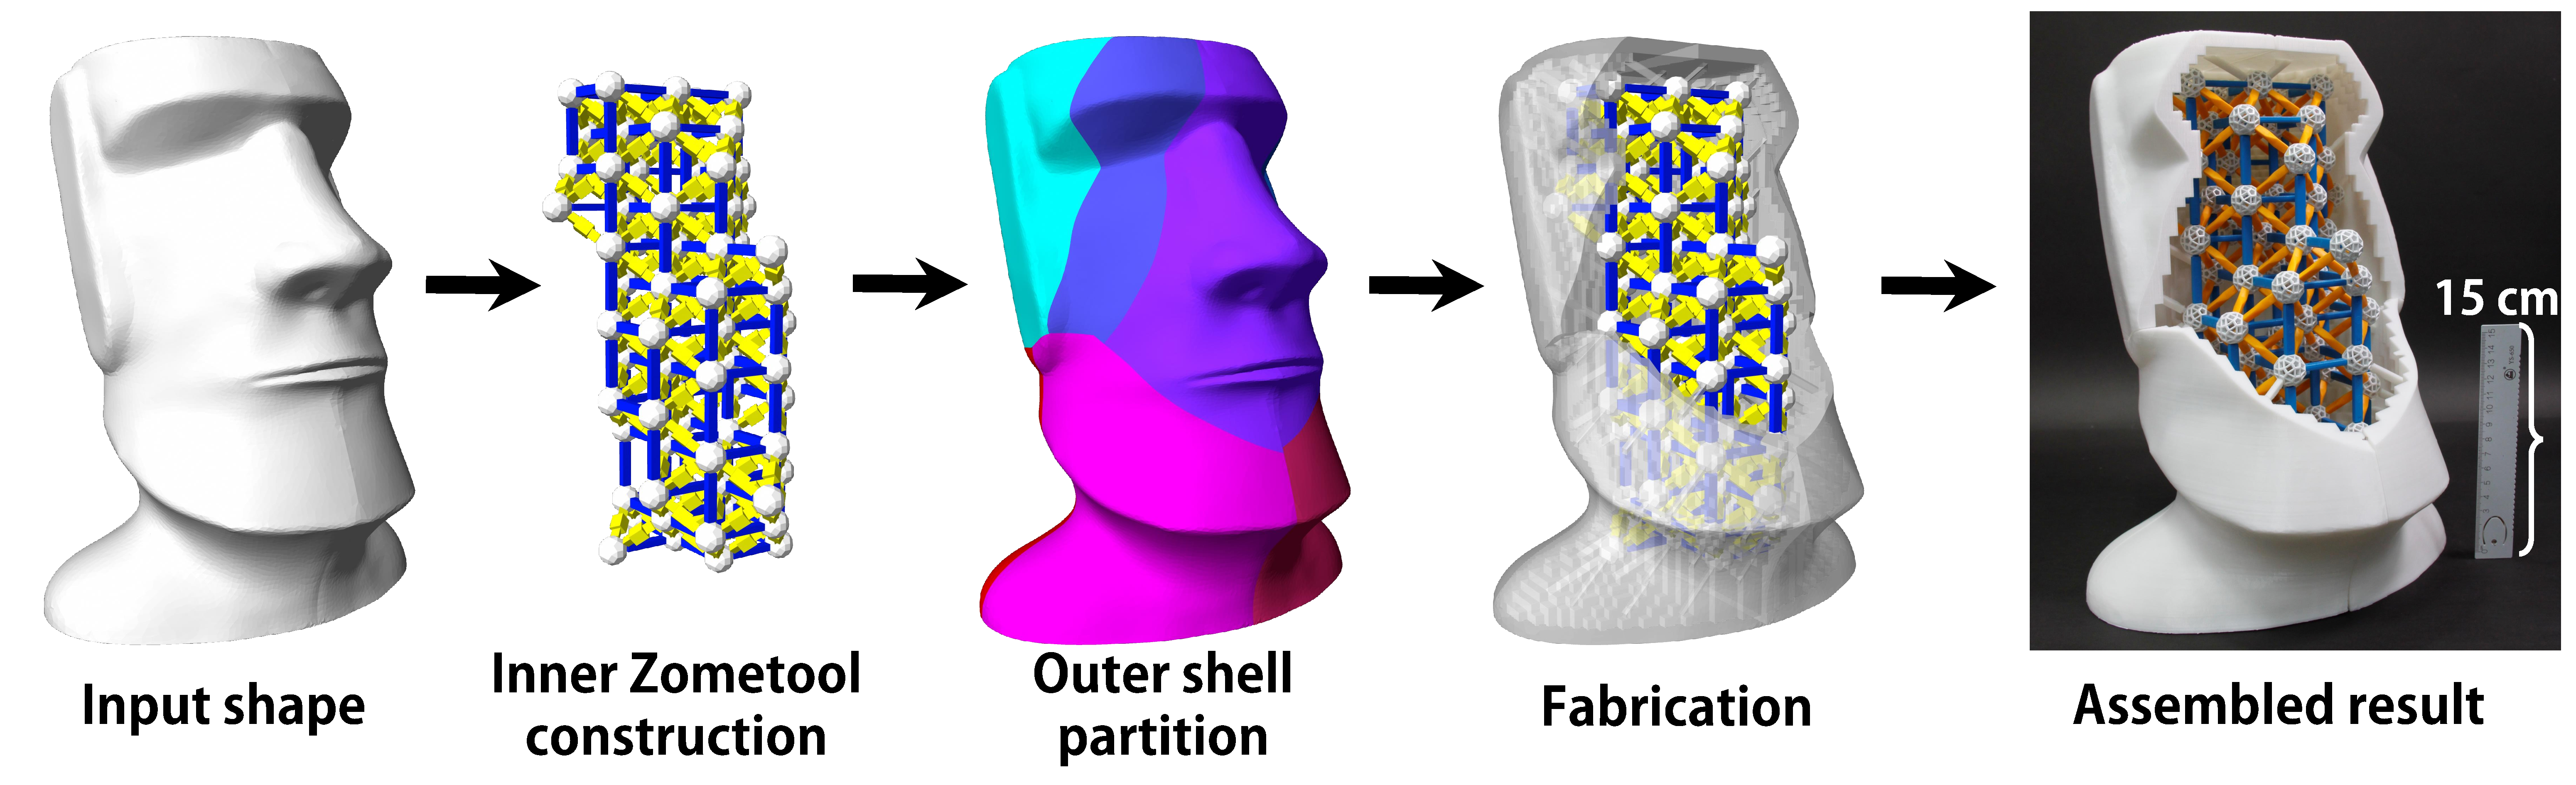
\includegraphics[width=16cm]{figs/pipeline2.pdf}
%   \caption{The overview of our method. 
% Given input shape, we first optimize the inner Zometool structure (\secname~\ref{sec:Zometool}). Guided by optimized Zometool structure, we partition the outer shell (\secname~\ref{sec:surf_part}) and generate connectors for assembling both structures (\secname~\ref{sec:fab}).
% The final fabricated result is obtained by assembling both assembled Zometool structure and printed outer shell.}
% \label{fig:result-pipeline}
%   }

%% Uncomment below to disable the manuscript note
%\renewcommand{\manuscriptnotetxt}{}

%% Copyright space is enabled by default as required by guidelines.
%% It is disabled by the 'review' option or via the following command:
% \nocopyrightspace

%%%%%%%%%%%%%%%%%%%%%%%%%%%%%%%%%%%%%%%%%%%%%%%%%%%%%%%%%%%%%%%%
%%%%%%%%%%%%%%%%%%%%%% START OF THE PAPER %%%%%%%%%%%%%%%%%%%%%%
%%%%%%%%%%%%%%%%%%%%%%%%%%%%%%%%%%%%%%%%%%%%%%%%%%%%%%%%%%%%%%%%%

\begin{document}

%% The ``\maketitle'' command must be the first command after the
%% ``\begin{document}'' command. It prepares and prints the title block.

%% the only exception to this rule is the \firstsection command
% \firstsection{Introduction}

\maketitle
% \begin{abstract}
\abstract{
In recent years, personalized fabrication has attracted many attentions due to the widespread of consumer-level 3D printers.
However, consumer 3D printers still suffer from shortcomings such as \ignore{the relatively }long production time and limited output size, which are undesirable factors to large-scale rapid-prototyping.
In order to fabricate \chinky{a} large-scale object,\ignore{construct a large-scale fabrication, the hybrid approach is introduced.}
\ignore{In this paper, }
we propose a 3D fabrication method that combines 3D printing and Zometool structure for cost-effective fabrication of large objects.
The key of our approach is to utilize compact, \chireplace{solid}{sturdy} and re-usable internal structure (Zometool) to \chinky{infill fabrications and} replace \chiremove{the} both time and material-consuming 3D-printed materials.
\chireplace{And}{ Moreover, }as a result, we can \chireplace{greatly}{significantly} reduce the cost and time by printing \chiremove{a} thin 3D external shells only.
% The key of our approach is using Zometool as a compact and solid internal structure, and 
% to build internal structure
% then attach thin 3D-printed external shells.
We design an optimization framework to generate both Zometool structure and printed surface partitions by balancing between several criteria including printability, material saving, and Zometool structure complexity.
% We optimize these criteria and generate both the Zometool structures and the surface partitions.
We demonstrate the effectiveness of the proposed method by a variety of 3D models along with examples of the physically fabricated objects.

\noindent
{\bf Keywords:} Geometric Algorithms, Fabrication, Curve, surface, solid, and object representations.
}


% \end{abstract}
%\firstsection{Introduction}
%!TEX root = zomeFab.tex
\section{Introduction}
\label{sec:introduction}

% The production cost of 3D printer has been declining and it's availability for everyone leads to the emergence of large amount of applications. 
The recent widespread of consumer\chinky{-}level 3D printer lead to the emergence of large amount academic and industrial fabrication applications.
However, the consumer-level 3D printers have several shortcomings including long printing time, limited output size and \chinky{the } high cost of materials. 
In order to address these shortcomings, many of the researches are proposed.
% There are several approaches and researches aim to solve these drawbacks. 
For saving time and materials, the modern 3D printers allow user\chinky{s} to save materials by switching between different fill-rate settings.
Meanwhile, different internal patterns are proposed~\cite{Lu:2014:BSW} to save materials while maintain\chinky{ing} the \chireplace{structure}{structural} soundness.
% provide different fill-rate settings to use less material and research like~\cite{Lu:2014:BSW} can save materials effectively. 
% The size of objects that 3D printing can produce are typically limited by 3D printers. 
For building a large-scale fabrication, lots of research\chireplace{es}{} \cite{Medell:2007:ALRP, Hao:2011:APLM, Luo:2012:CPM, Hu:2014:APS, Vanek:2014:PMVO} focus on this problem and share the spirit of partitioning the object into sub-part\chinky{s} that can be fitted into printing volume.
% They all have same characteristic that partition the object to fit the size, then assembling printed parts.

% The requirements for a large-scale fabrication will enlarge the drawbacks as mentioned above.
However, the saving of time and material from existing methods are still not sufficient for large-scale shape fabrication.
% It turns out that even we employ state-of-the-art methods, time and material spending are still too high. 
\chireplace{To decrease cost extremely}{To immensely decrease the cost}, our novel idea is to combine 3D printing with another structure. 
That desire structure must meet several criteria such as (i) easy to assemble, (ii) re-usable, and (iii) robustness, so that the resulted fabricated shape is simple to build and reliable simultaneously. 
Base on our requirements, the popular modeling system, \ie~\emph{Zometool}~\cite{davis2007mathematics}, is suitable for coarse fabrication.
In addition to the above advantages, \emph{Zometool} still has several \chireplace{good}{excellent} characteristics: 
(i) structural properties, such as stability, expandability and lightness satisfying the requirements for large-scale fabrication. 
(ii) Independent structure and modularity can parallelize the construction to speed up the building process.
Hence, Zometool is a \chireplace{good}{attractive} candidate to replace solid 3D printing material as the \chireplace{inner robust}{robust inner} structure of large-scale structure.
Therefore, the goal of this work is to develop a computational method that combines Zometool structure and 3D printing to reduce the time and material costs in large-scale fabrication.
% In this paper, we present a novel method, called ZomeFab, that can automatically generate both outer shell and inner Zometool structures approximating to a given 3D input mesh.
Given the desired 3D shape, we design an optimization process to synthesize the inner Zometool structure, which balance\chinky{s} between the shape similarity and structure complexity.
We leverage Simulated Annealing to explore the huge structure space effectively.
% We first perform mesh segmentation to split the complex 3D mesh into different shape parts.
% For each part, we fit the smallest cube of Zometool structure as initial inner structure.
% From the initial Zometool structure, we use Simulated Annealing algorithm to effectively explore the huge structure space.
Next, with the optimized Zometool structure, we hollowed the shape to obtain the outer shell and partition the outer shell \chireplace{with respect to}{concerning} several criteria including simplicity and printability.
We formulate these criteria in a single MRF problem and solve it with graph-cut algorithm~\cite{boykov:2004:experimental}.
We also design a \chireplace{special}{particular} type of connectors \chireplace{and}{furthermore,} optimize their positions for assembling the inner Zometool structure and outer shell.

There are two primary contributions in this paper:
\begin{enumerate}
\item We propose an optimization framework to synthesize the inner Zometool structure to replace the solid printed materials in large-scale fabrication, which greatly reduce the printing cost including time and materials.
% Filled by Zometool structure instead of solid printed is greatly reduce the printing cost including time and materials.
\item We design and print a special connector and optimize their layout for better combining both inner Zometool structure and outer printed shell.
\end{enumerate}

% The rest of this paper is organized as follows. In  \secname~\ref{sec:relatedwork}, we surveyed several previous methods for computational fabrication and applications of modeling system Zometool.  \secname~\ref{sec:Zometool}, \secname~\ref{sec:surf_part} and \secname~\ref{sec:fab} describe the three main stages of our method: \emph{Zometool construction}, \emph{surface partition} and \emph{Fabrication}, respectively. In \secname~\ref{sec:result}, we demonstrate the results of our method.
% Finally, we make a conclusion in  \secname~\ref{sec:conclusion}.

%\firstsection{Introduction}
%!TEX root = zomeFab.tex
\section{Related Work}
\label{sec:relatedwork}

\subsection{Computational Fabrication}
In recent years, computational fabrication has attracted many attentions in the computer graphics and human computer interaction research fields~\cite{Shamir:2016:CTP}.
Numerous works are proposed to fabricate shapes 
(i) with different objectives, e.g. maintain balance~\cite{Prevost:MIS:2013,SpinIt:Baecher:2014}, reduce size~\cite{Luo:2012:CPM}, strengthen structure soundness~\cite{Zhou:2013:WSA} and generate specific sounds~\cite{Umetani:2016:PIR}, and 
(ii) with different materials or building blocks, e.g. Lego~\cite{Luo:2015:LOL}, planar slices~\cite{Cignoni:2014:FMJ}, and interlocking puzzles~\cite{Song-2012-InterCubes}.

However, even with the fast developments of assist tools and algorithms, 3D printers still suffer from long production time, excessive material usage, and limited output size.
To reduce the usage of print materials, Huang~\cite{Huang:2016:FRF} and Wu~\cite{Wu:2016:PAM} design devices and algorithms to print shapes in wireframe.
Meanwhile, different internal structures are developed, e.g. the skin-frame structure~\cite{Wang:2013:CPO}, the honeycomb-like structure~\cite{Lu:2014:BSW}, and 2D laser cutting shape proxy~\cite{Song-2016-CofiFab}.
To enable the large shape to be printed using 3D printers, Luo~\etal~\cite{Luo:2012:CPM} developed an iterative planar-cut method, aiming to fit decomposed parts in the 3D printing volume while considering factors such as assembility and aesthetics.
Yao~\etal~\cite{Yao:2015:LPP} proposed a level-set framework for 3D shape partition and packing.
Compared to these works, our method fabricate a shape with both Zometool structure and 3D-printed parts, so that we can reduce the fabrication time and cost, with the reusability of Zometool structures. 

\subsection{Zometool Design and Modeling}
Zometool is a mathematically-precise plastic construction set for building a myriad of geometric structures~\cite{davis2007mathematics}, from simple polygons to visualize and model various natural sciences, e.g. DNA molecules.
It's history dated back to to the 1960s where it started out as a simple construction system inspired by Buckminster Fulleresque geodesic domes, and it evolved from simple toy to versatile modeling tools through years.
Although we can use it to construct complex structure, it's not intuitive for naive users to use and meanwhile time-consuming.

Tools are developed to help users to design the Zometool structures, e.g. vZome \cite{SVZ} and ZomeCAD \cite{ESZ}.
These systems provide different ways to grow the structure.
However, the difficulties remain when it comes to build a complex structure because it lacks the ability to provide useful suggestions about what kinds of structure to use next in order to build the target shape.

This motivates works toward automatic construction through computational method.
Zimmer~\cite{zimmer:2014:Zometool,zimmer:2014:tvcg} approximate and realize freeform surface automatically using Zometool.
Zimmer~\cite{zimmer:2014:tvcg} adopt an incremental panels growing strategy to approximate the surface without self-collisions.
On the other hand, Zimmer~\cite{zimmer:2014:Zometool} first build up a rough initial Zometool structure and explore the modification space using local operations. The final Zometool structure is obtained by a stochastic optimization framework.

\subsection{Mesh Segmentation}
Mesh Segmentation is an important step for decreasing the complexity of the mesh by splitting the original mesh into many small segments. 
There are a lot of 3D mesh segmentation algorithms which have been proposed, including K-means~\cite{shlafman:2002:metamorphosis}, graph cuts~\cite{boykov:2004:experimental, golovinskiy:2008:randomized}, primitive fitting~\cite{attene2006hierarchical}, random walks~\cite{lai2008fast}, core extraction~\cite{katz2005mesh}, spectral clustering~\cite{liu2004segmentation}, critical point analysis~\cite{lin2007visual}, Shape Diameter Function~\cite{shapira:2008:consistent}, and SVM planar cut~\cite{wang2016improved}.

In our method, we intend to segment shape so that the resulted segments are printable by the 3D printer, and meanwhile is able to be connected to the internal Zometool structure.
% Our purpose of segmentation is for 3D printing for user to assemble the separate pieces, so we select two methods, graph cuts~\cite{boykov:2004:experimental, golovinskiy:2008:randomized} and SVM planar cut~\cite{wang2016improved}. 
We achieve this by designing a two stages process that combines the advantages of MRF-based method~\cite{boykov:2004:experimental} and SVM planar cut~\cite{wang2016improved}.
The final segmented parts can be easily assembled with optimized Zometool structure.
% The method of graph-cuts ~\cite{boykov:2004:experimental} helps us classify the triangele of mesh to the Zome-ball of inner structure. 
% However, most segmentation methods just classify the triangle of mesh and we can't get the smooth edges. 
% It hard for user to assemble the pieces which have the sharp edges, so the method of planar cut is our first choice. 
% The method of SVM planar cut~\cite{wang2016improved} describes the SVM classifier can get the split plane from different labels of data. Finally, we combine two of the segmentation methods to get our mesh segment for user to assemble it.


%We reference the open source software Blender~\cite{BLD}, which have the function


\section{Overview}
\label{sec:overview}

% \begin{comment}
\begin{figure*}[h]
\centering
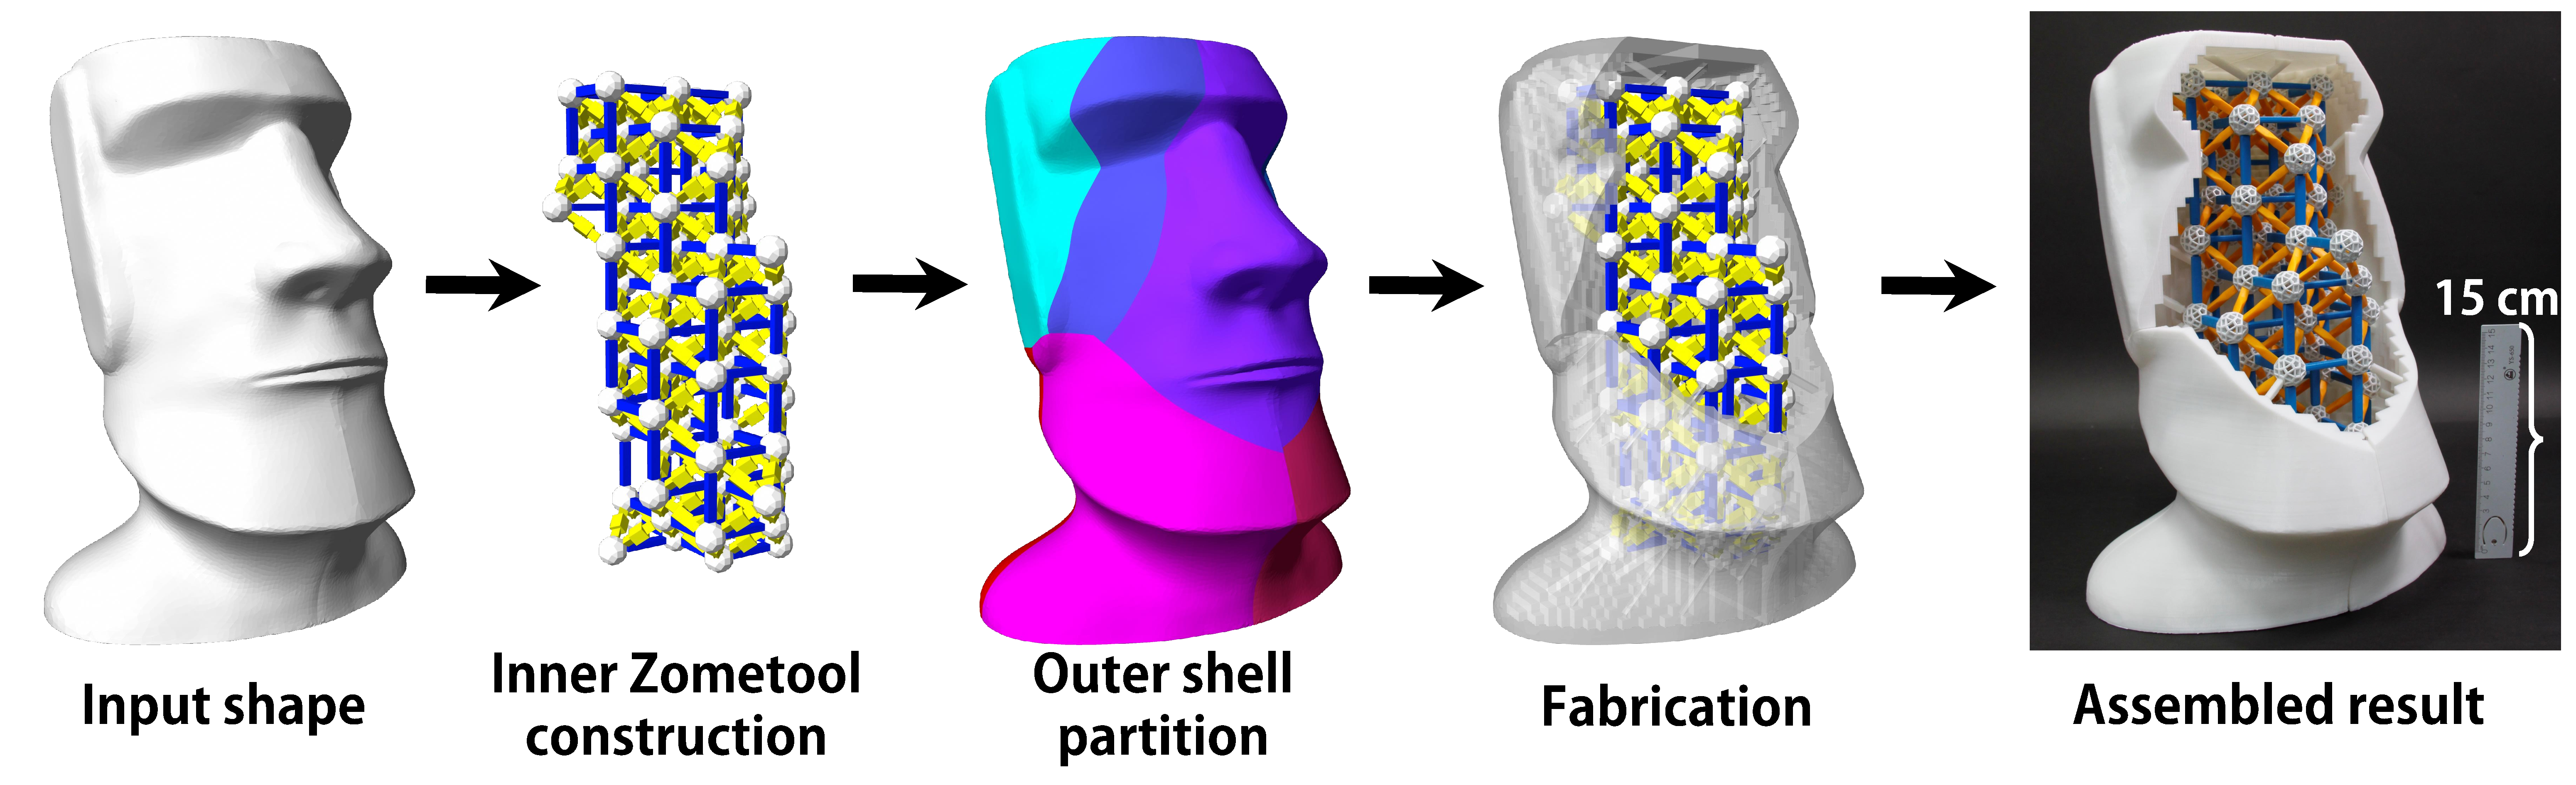
\includegraphics[width=1.0\linewidth]{figs/pipeline2.pdf} 
\caption{
Given input shape, we first optimize the inner Zometool structure (\secname~\ref{sec:Zometool}). Guided by optimized Zometool structure, we partition the outer shell (\secname~\ref{sec:surf_part}) and generate connectors for assembling both structures (\secname~\ref{sec:fab}).
The final fabricated result is obtained by assembling both assembled Zometool structure and printed outer shell.
}
\label{fig:result-pipeline}
\end{figure*}
% \end{comment}

Given a 3D shape, our method automatically generate\chinky{s} inner Zometool structure and outer 3D-printed shells.
% Zomefab is a method which combines Zometool and 3{D} printing for large-scale fabrication. 
Our method has the following features:
\begin{enumerate}
\item \textbf{Large Object.} Our method aim\chinky{s} for fabricating the large-scale object which it's height is from 0.3 to 1 meters, which is way larger than the printing volume of \chireplace{common}{ordinary} consumer-level 3{D} printer.
\item \textbf{Fabricability.} Each segment of the outer shell can be printed and fitted inside the volume of consumer-level 3{D} printer\chinky{s}.
\item \textbf{Assemblability.} The inner Zometool structure can be easily assembled and connected to the outer printed shells using
\chireplace{special}{specifically} designed connectors.
% 3{D} printing segments can assemble onto the inner structure.
\item \textbf{Cost-effectiveness.} Our method maximize\chinky{s} the inner structure and minimize the printing materials. 
It decreases the fabrication time and the cost of materials.
\end{enumerate}

\chireplace{Our method is illustrated in~\figname~\ref{fig:result-pipeline}.}{\figname~\ref{fig:result-pipeline} illustrates our method.}
% There is a flow chart at \figname~\ref{fig:result-pipeline}.
Given the input shape, we voxelize the inner volume of the input mesh to get the result of \chinky{an} initial Zometool structure.
Our goal is to grow the Zometool structure to occupied the maximum inner volume \chireplace{in order}{} to reduce most of the printing materials.
% get the maximum inner structure, but the structure of initial guess is too far from surface. 
Therefore, we design an optimization framework using simulated annealing, and design several local operations to explore the feasible Zometool structure space.
After the optimization, we get the maximum inner structure (\secname~\ref{sec:Zometool}).

Next, in order to print the outer shell of input shape, we have to (i) partition the shape into pieces where each piece can be fitted into printing volume, (ii) put connectors at feasible locations so that the inner Zometool structure and the outer shells can be connected robustly, and (iii) keep the salient region\chinky{s} intact.
We formulate the partition problem as \chireplace{a}{an} MRF problem and solve it with graph cut algorithm.
The intuition of this formulation is that each triangle should be connected to it's closest Zomeball, but simultaneously we want to reduce the number of partitions and maintain the integrity of salient region.
To further regularize the resulted partitions, we apply the SVM algorithm to find the hyperplane  between different labels and also use the hyperplane for our cut-plane to separate the mesh ( \secname~\ref{sec:surf_part}).
% we assign the triangle to it's nearest Zome-ball, but the number of labels is too much. 
% Hence, we use graph cut algorithm to help us optimize the classification and get the suitable number of labels. After the classification, we use Support Vector Machine classifier find the hyperplane between different labels and also use the hyperplane for our cut-plane to separate the mesh. (see \secname~\ref{sec:surf_part})

Last, before we separate the mesh by our cut-plane, we generate the inner surface by voxelizing the inner volume, and combine with the outer mesh as the solid mesh. 
% We voxelize inner volume of original mesh, and combine the result of voxelization, also the original mesh will become the new mesh. 
Then, we apply all cut planes on the solid\ignore{new }mesh and get the separate pieces. 
% But so far we just have the pieces, so 
We design the special connector and connect the pieces to the inner Zometool structure. 
Finally, the pieces with connectors can be printed and assembled to get the final large-scale object (\secname~\ref{sec:fab}).
% user gets the pieces with connector and assemble all of pieces to the inner structure, so that we can get the large-scale object by our method (\secname~\ref{sec:fab}).
\section{Zometool construction}
\label{sec:Zometool}

% \begin{figure}[ht]
% \centering
% 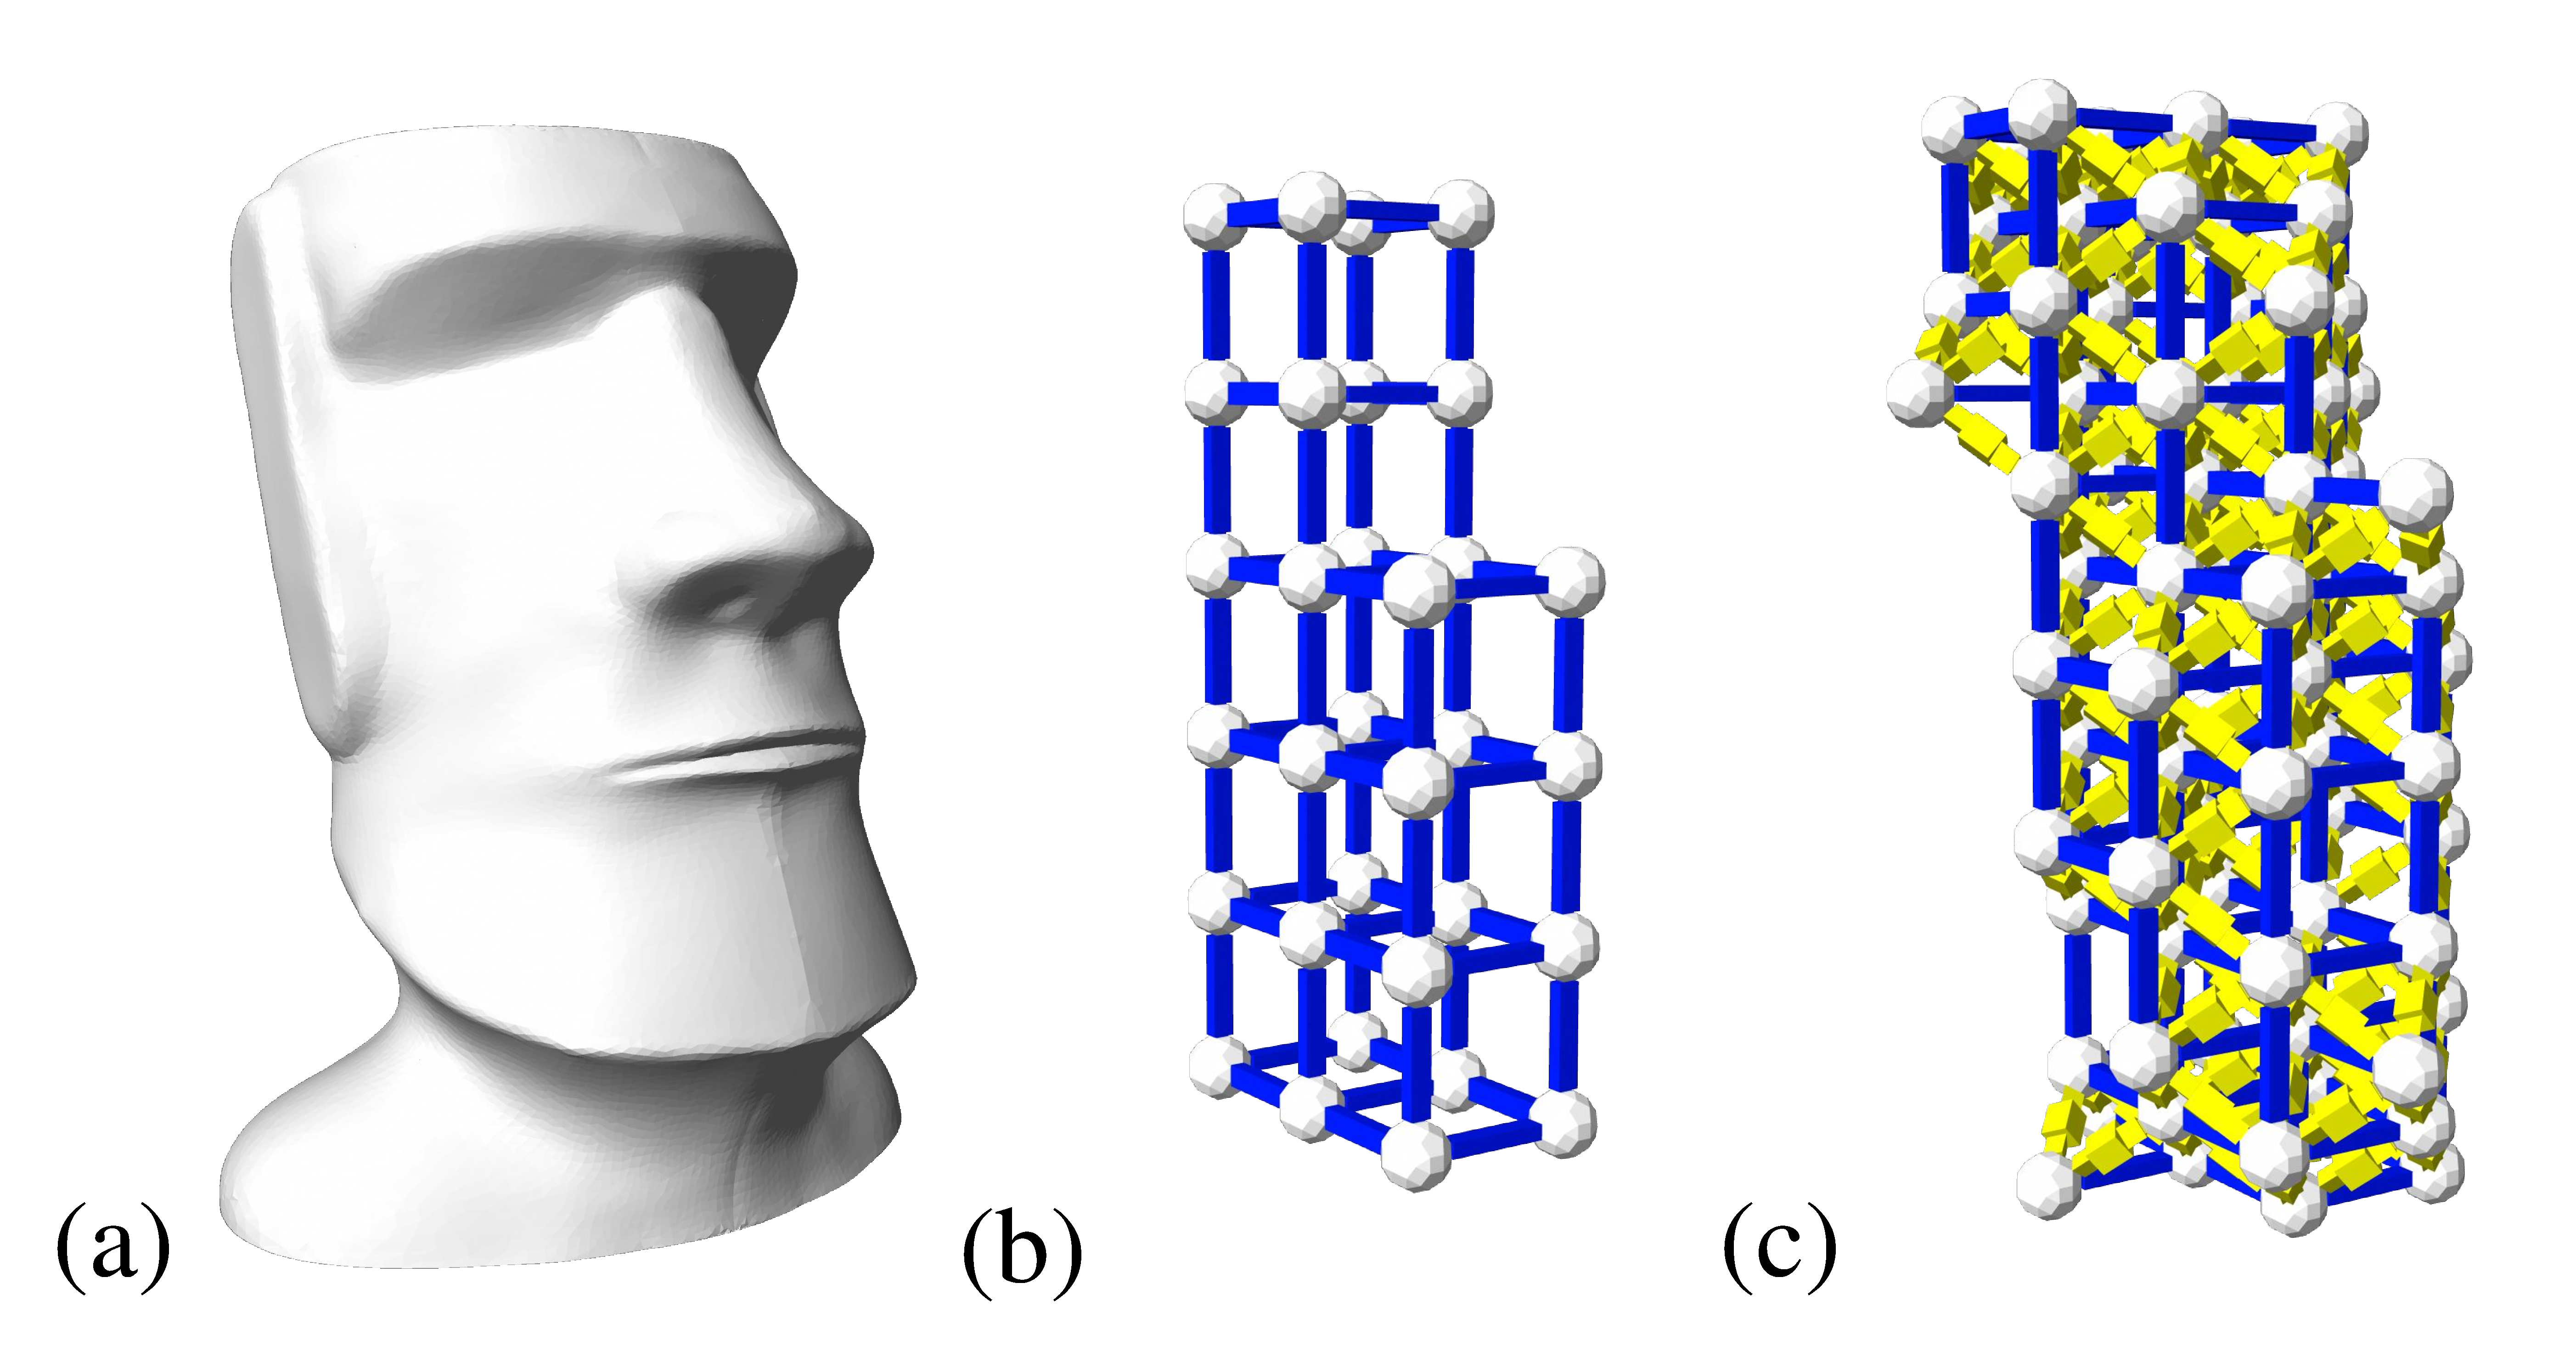
\includegraphics[width=\linewidth]{figs/Zometool_init.pdf} 
% \caption{
% \ichao{this figure is too space wasting..Maybe just put a small cube as inset in the corresponding location in paper.}
% Given input shape (a), we initialize the Zometool structure with cubes (b), and obtain the optimized result (c) by using Simulated Annealing as described in \secname~\ref{sec:Zometool}.}
% \label{fig:Zometool_cont}
% \end{figure}

% The goal of our method is devising an algorithm to construct an object composed of Zometool structures and 3D-printed parts with the following objectives:
% \begin{itemize}
%     \item \textit{material-effecitiveness} We should aim to minimize the overall fabrication cost and time.
%     Since Zometool is substantially faster to build and reusable, we should maximize it's usage to reduce 3D printing material in the fabrication.
%     \item \textit{easy-to-assemble} We should reduce the difficulties of assemble both Zometool structure and outer printed shell. In terms of Zometool, we should minimize the usage of nodes and rods, so to reduce the assemble time.
% \end{itemize}

% \begin{figure}[ht]
% \centering
% 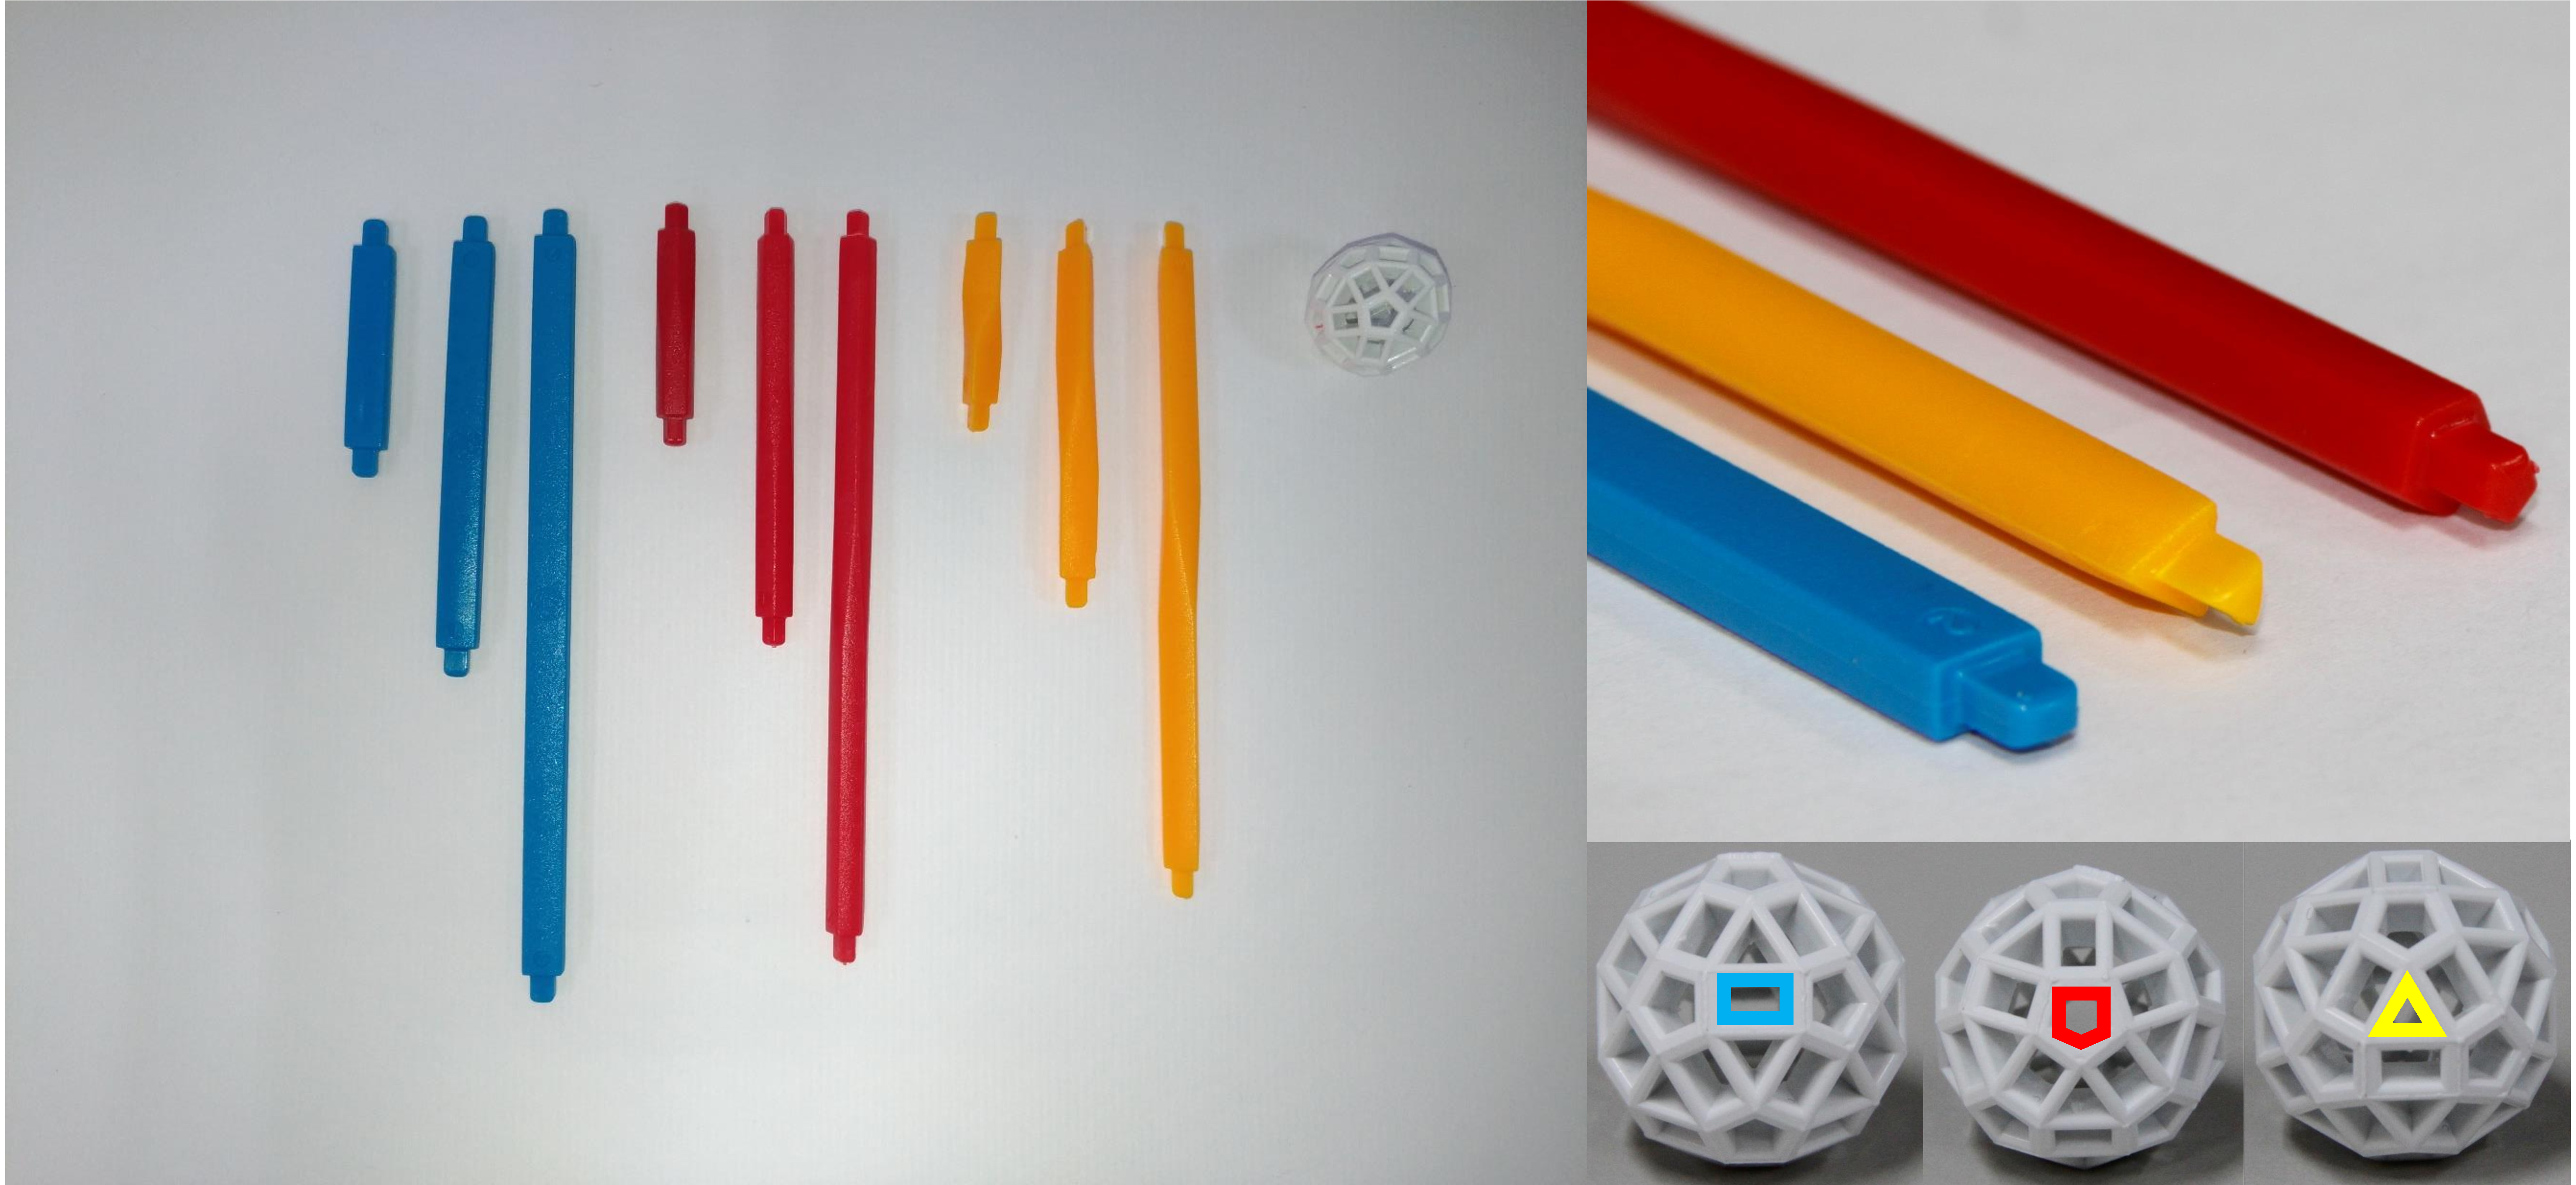
\includegraphics[width=1.0\linewidth]{figs/Zometool.pdf} 
% \caption{
% The standard Zometool components}
% \label{fig:Zometool}
% \end{figure}

\begin{wrapfigure}{R}{0.3\textwidth}
\centering
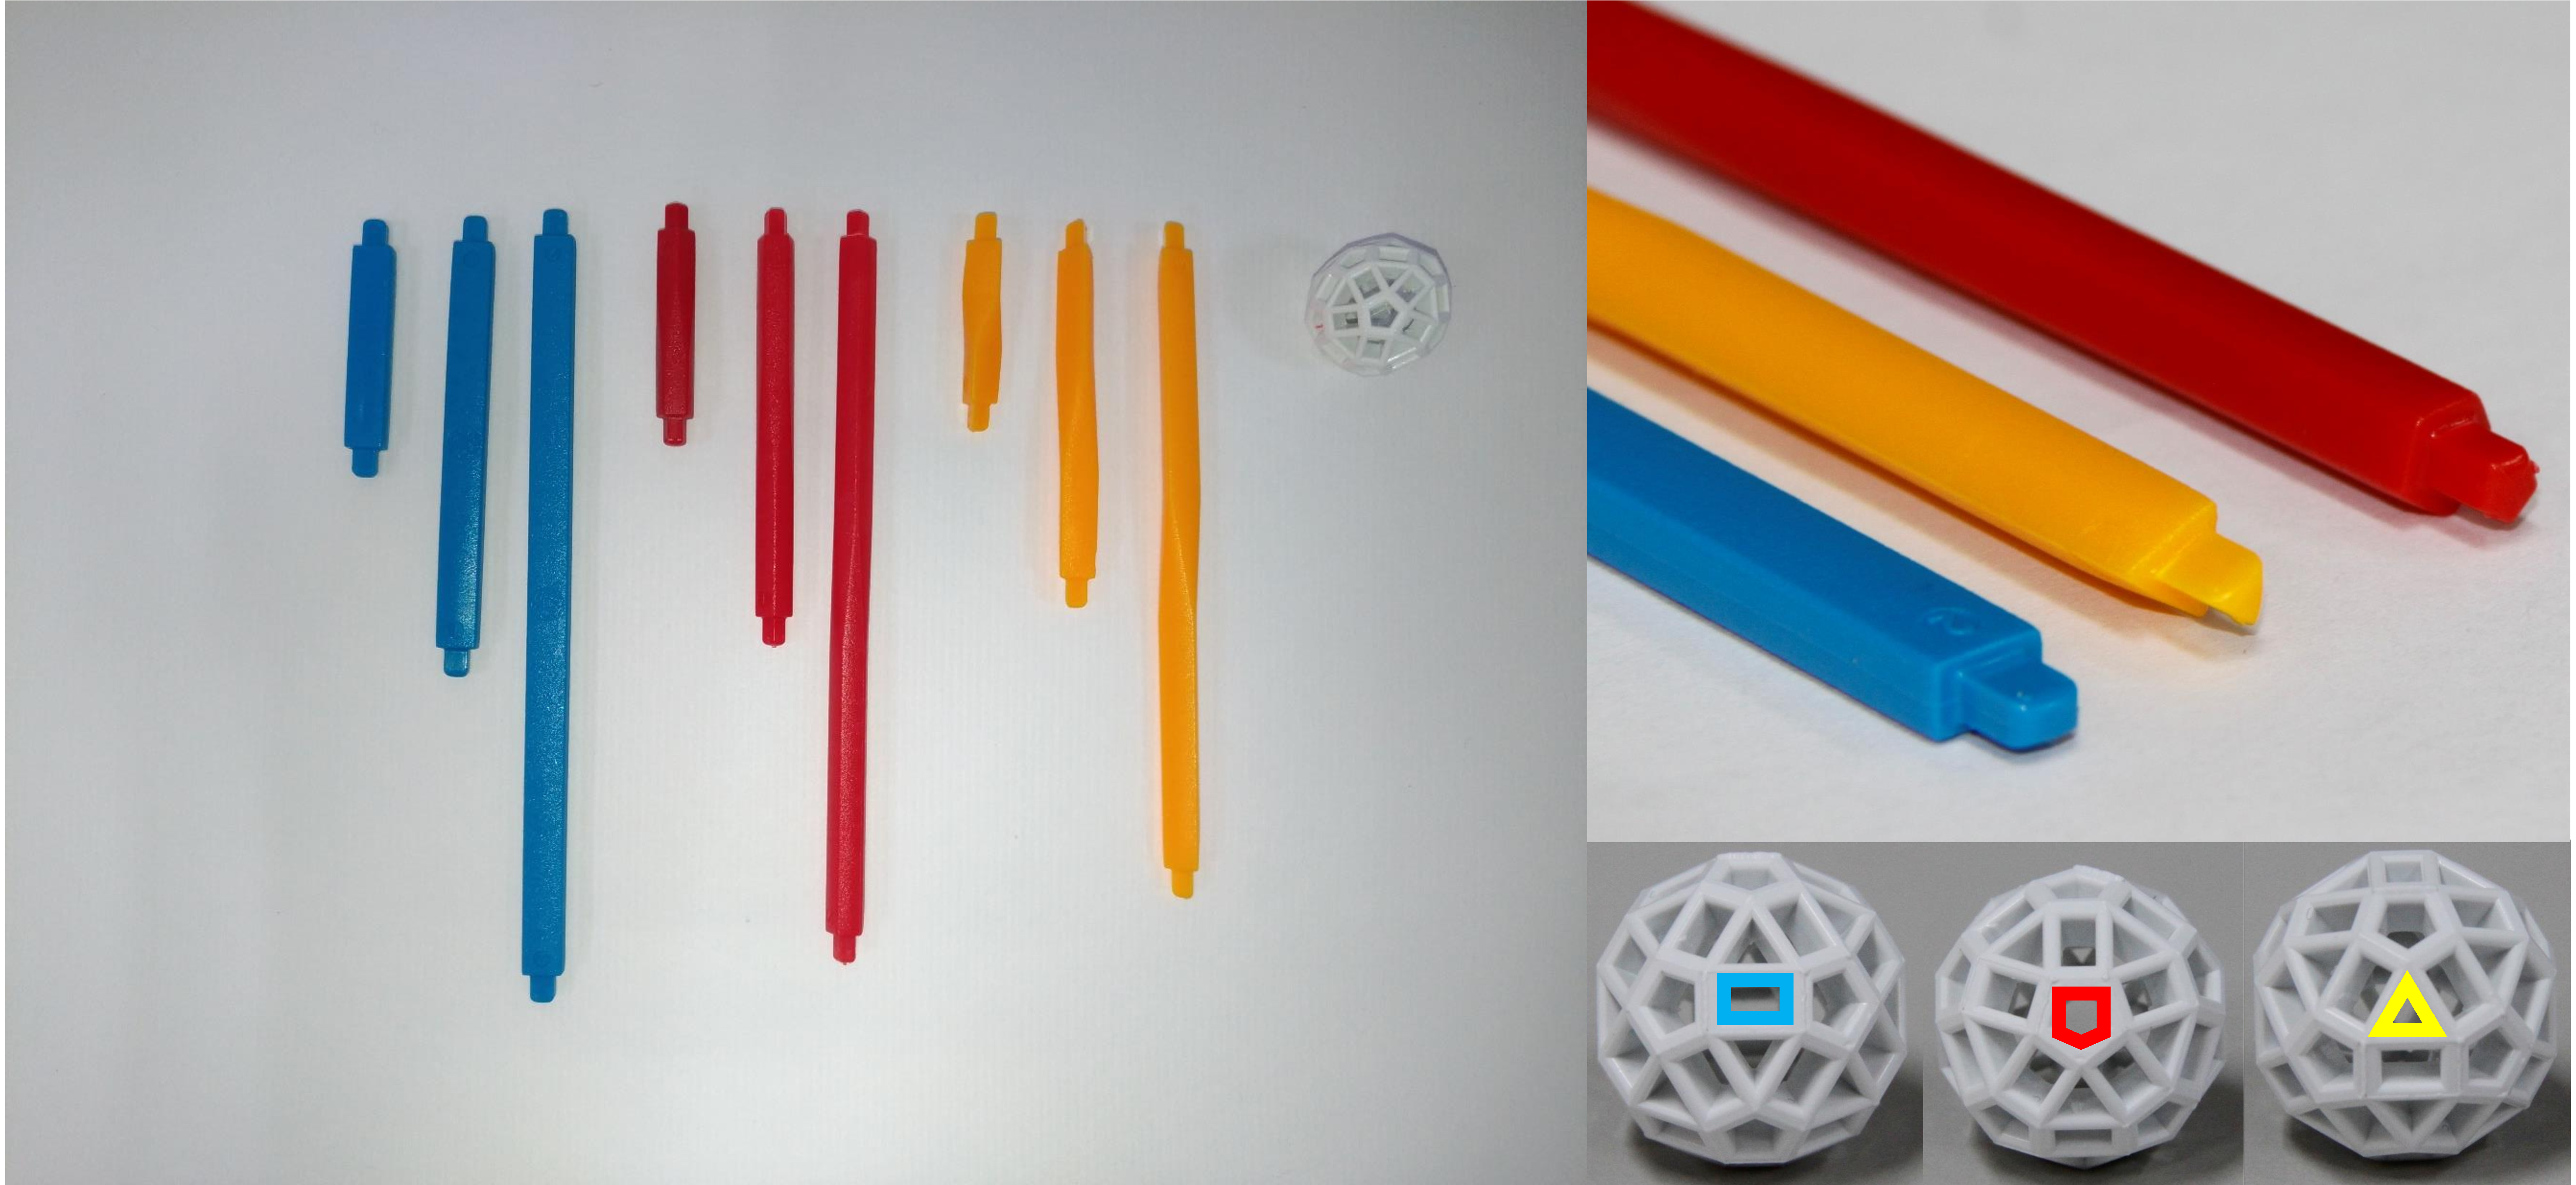
\includegraphics[width=0.3\textwidth]{figs/Zometool.pdf}
% \caption{The standard Zometool components}
\label{fig:Zometool}
\end{wrapfigure}

\subsection{Introduction to Zometool}
Zometool is widely used as educational toys to replicate complicated scientific structures such as chemical structures. 
The rods in standard Zometool system have three different types tenons, \ie~blue for rectangle, red for pentagonal and yellow for triangle.
Each type of rod also has three different sizes (see inset).
We denote $(b_0$, $b_1$, $b_2)$ as three different lengths of blue rods ($(r_0$, $r_1$, $r_2)$ for red rod, and $(y_0$, $y_1$, $y_2)$ for yellow rod).
% Also, $r_0$, $r_1$, $r_2$ are the red rods, and $y_0$, $y_1$, $y_2$ are for yellow rods. 
There are totally 62 slots on the Zome-ball, including 30 rectangular slots, 12 pentagonal slots and 20 triangular slots. 
% On the other hand, Zometool has a math model which we will introduce it's detail in following context.
%The Zome-ball have 62 slots on it. There are 30 rectanglular slots, 12 pentagonal slots and 20 triangular slots. Zometool have a math model in it. We will introduce it's detail in following context.
% \subsubsection{Strut lengths}
Each color of Zometool rods has three sizes, and the growing ratio is related to the golden ratio $\gamma = \frac{1+\sqrt{5}}{2}$. 
Take blue rods for example, $b_1 = b_0 \cdot \gamma$ and $b_2 = b_0 + b_1$. 
Red and yellow rods also follow this rule. 
Moreover, the relative length ratios are different from yellow to blue and red to blue, \ie~ $y_i = \frac{\sqrt{3}}{2} \cdot b_i$ and $r_i = \frac{\sqrt{2 + \gamma}}{2} \cdot b_i$.
Please refer to~\cite{davis2007mathematics} for more detail about the underlying mathematical model of Zometool.
% Moreover, the rods with different colors have their own related ratio, i.e. $y_i = \frac{\sqrt{3}}{2} \cdot b_i$ and $r_i = \frac{\sqrt{2 + \gamma}}{2} \cdot b_i$.

% \subsubsection{Zometool vectors}
% Now we know Zome-ball have 62 slots on it, and there are three different types of rods. 
% Each type of them has three different sizes. 
% If we put the Zome-ball in x-y-z coordinate, we can get 62 fix vectors which correspond to slots. And we also can get 186 positions which is from the center of Zome-ball to the end point of rods. This information can improve the accuracy in computation.

% \begin{figure}[ht]
% \centering
% 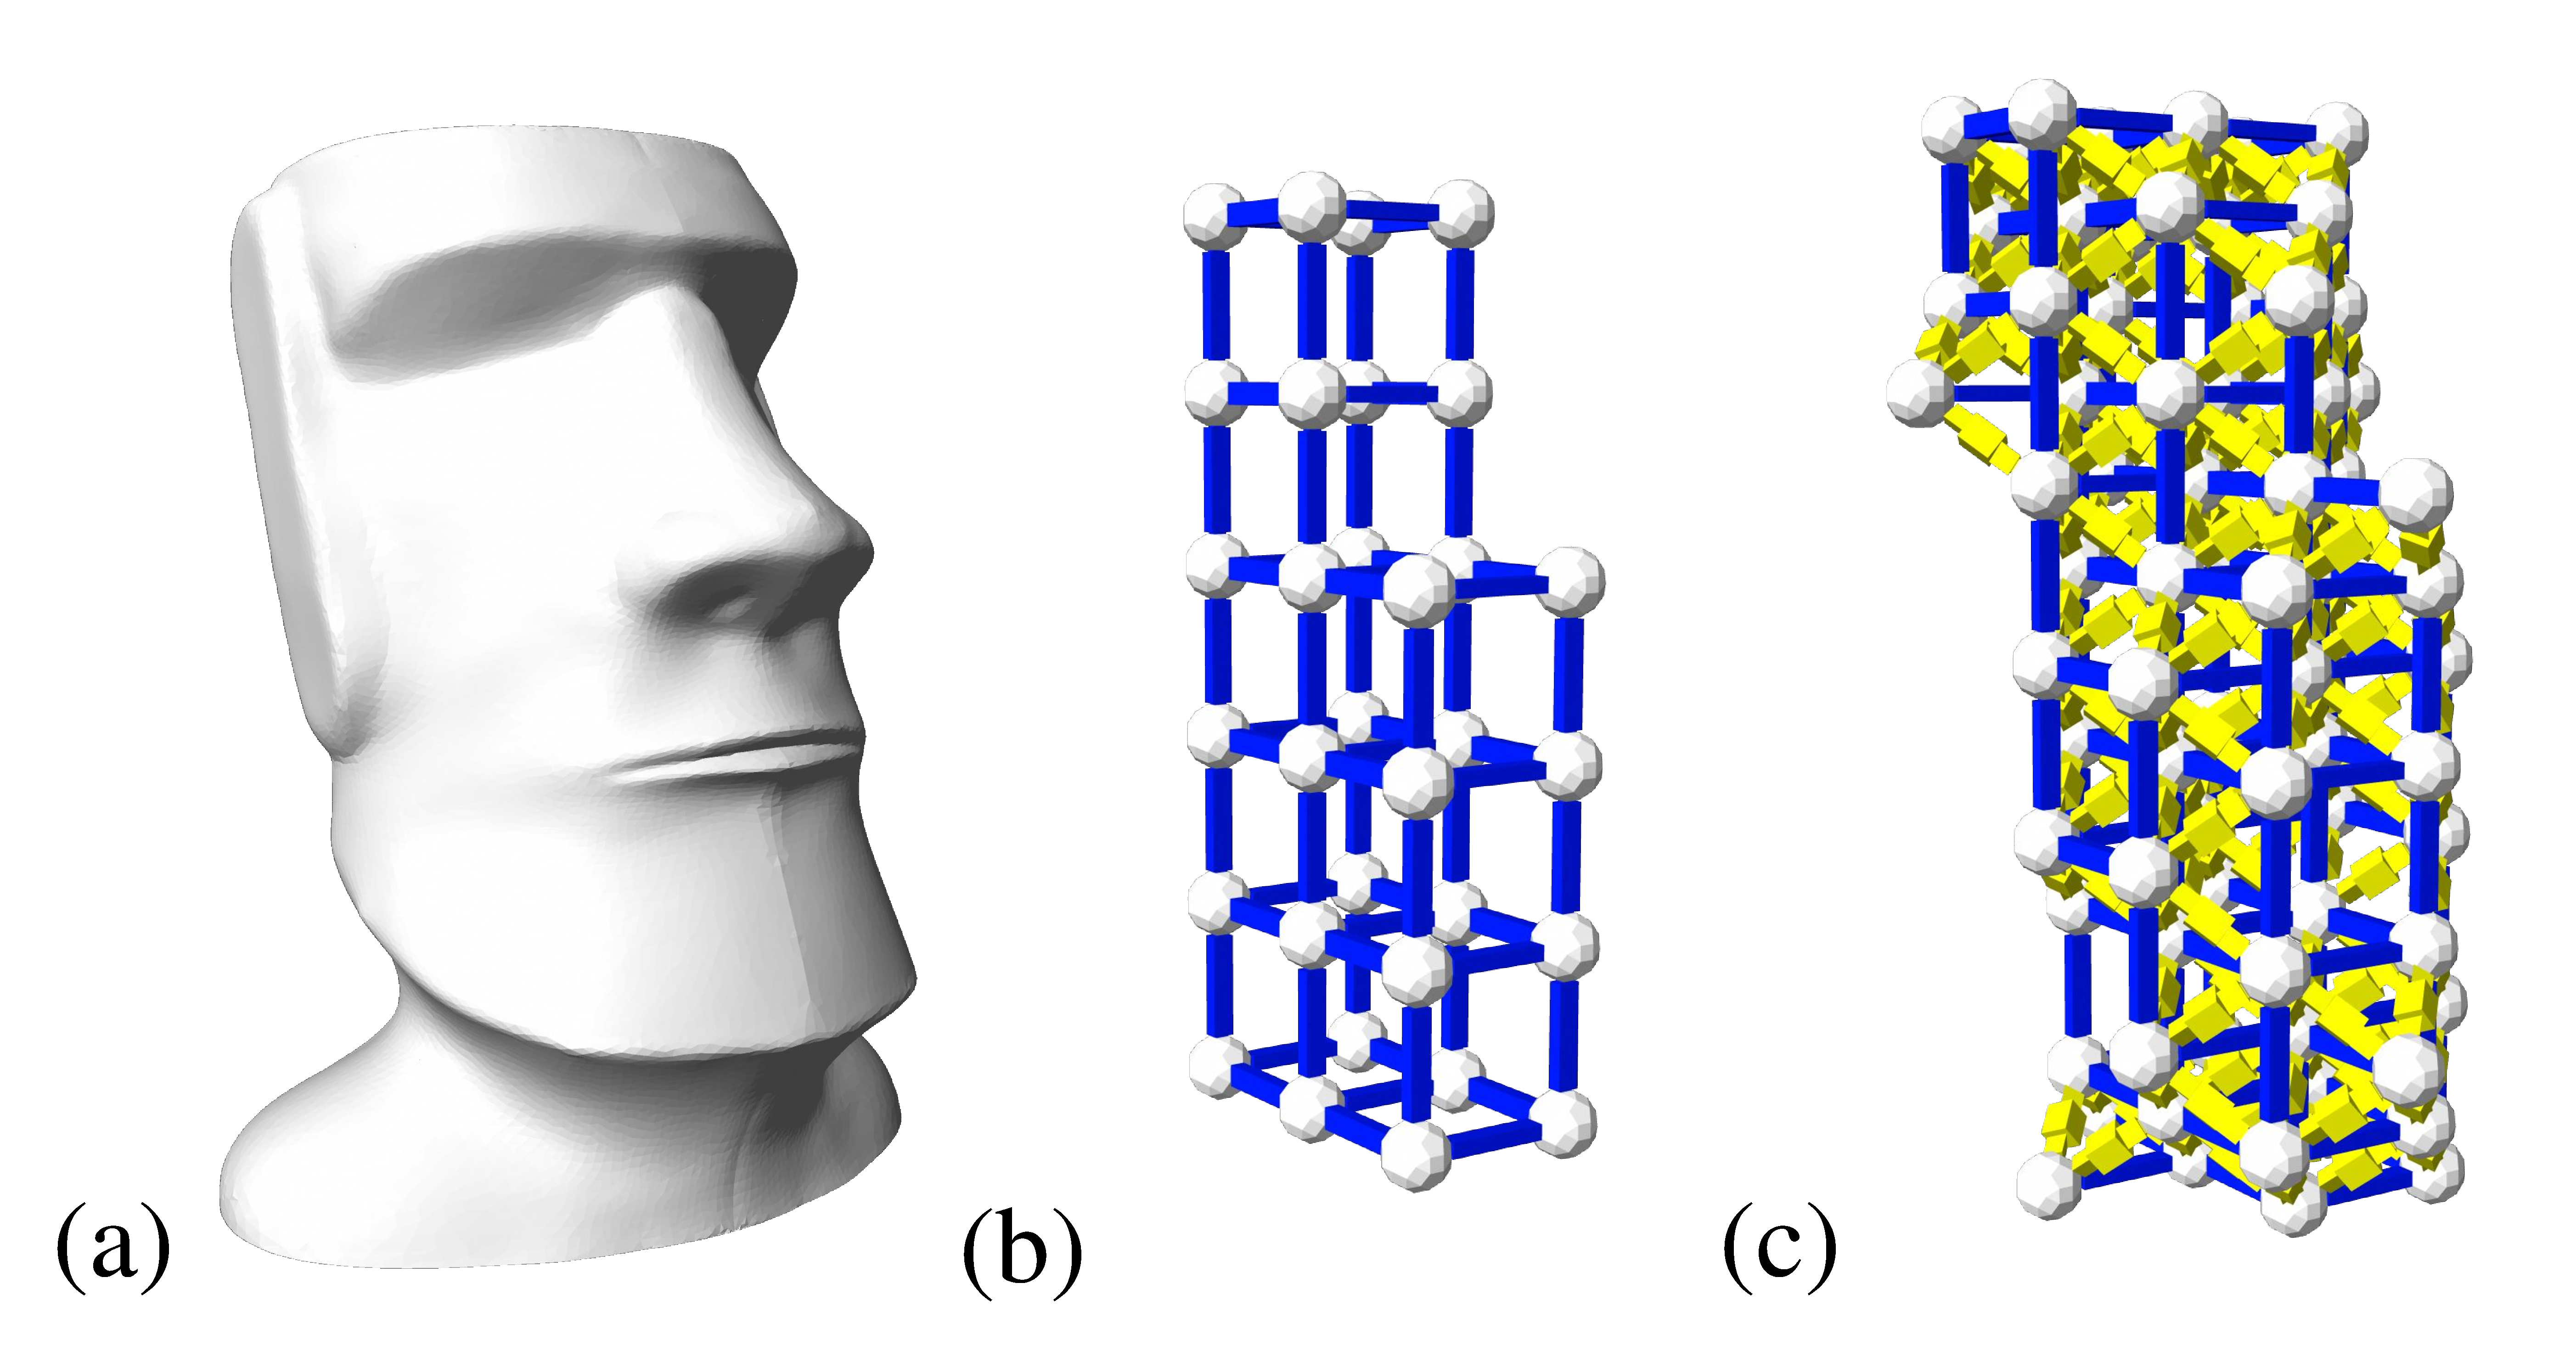
\includegraphics[width=\linewidth]{figs/Zometool_init.pdf} 
% \caption{
% \ichao{this figure is too space wasting..Maybe just put a small cube as inset in the corresponding location in paper.}
% Given input shape (a), we initialize the Zometool structure with cubes (b), and obtain the optimized result (c) by using Simulated Annealing as described in \secname~\ref{sec:Zometool}.}
% \label{fig:Zometool_cont}
% \end{figure}

\begin{wrapfigure}{R}{0.1\textwidth}
\centering
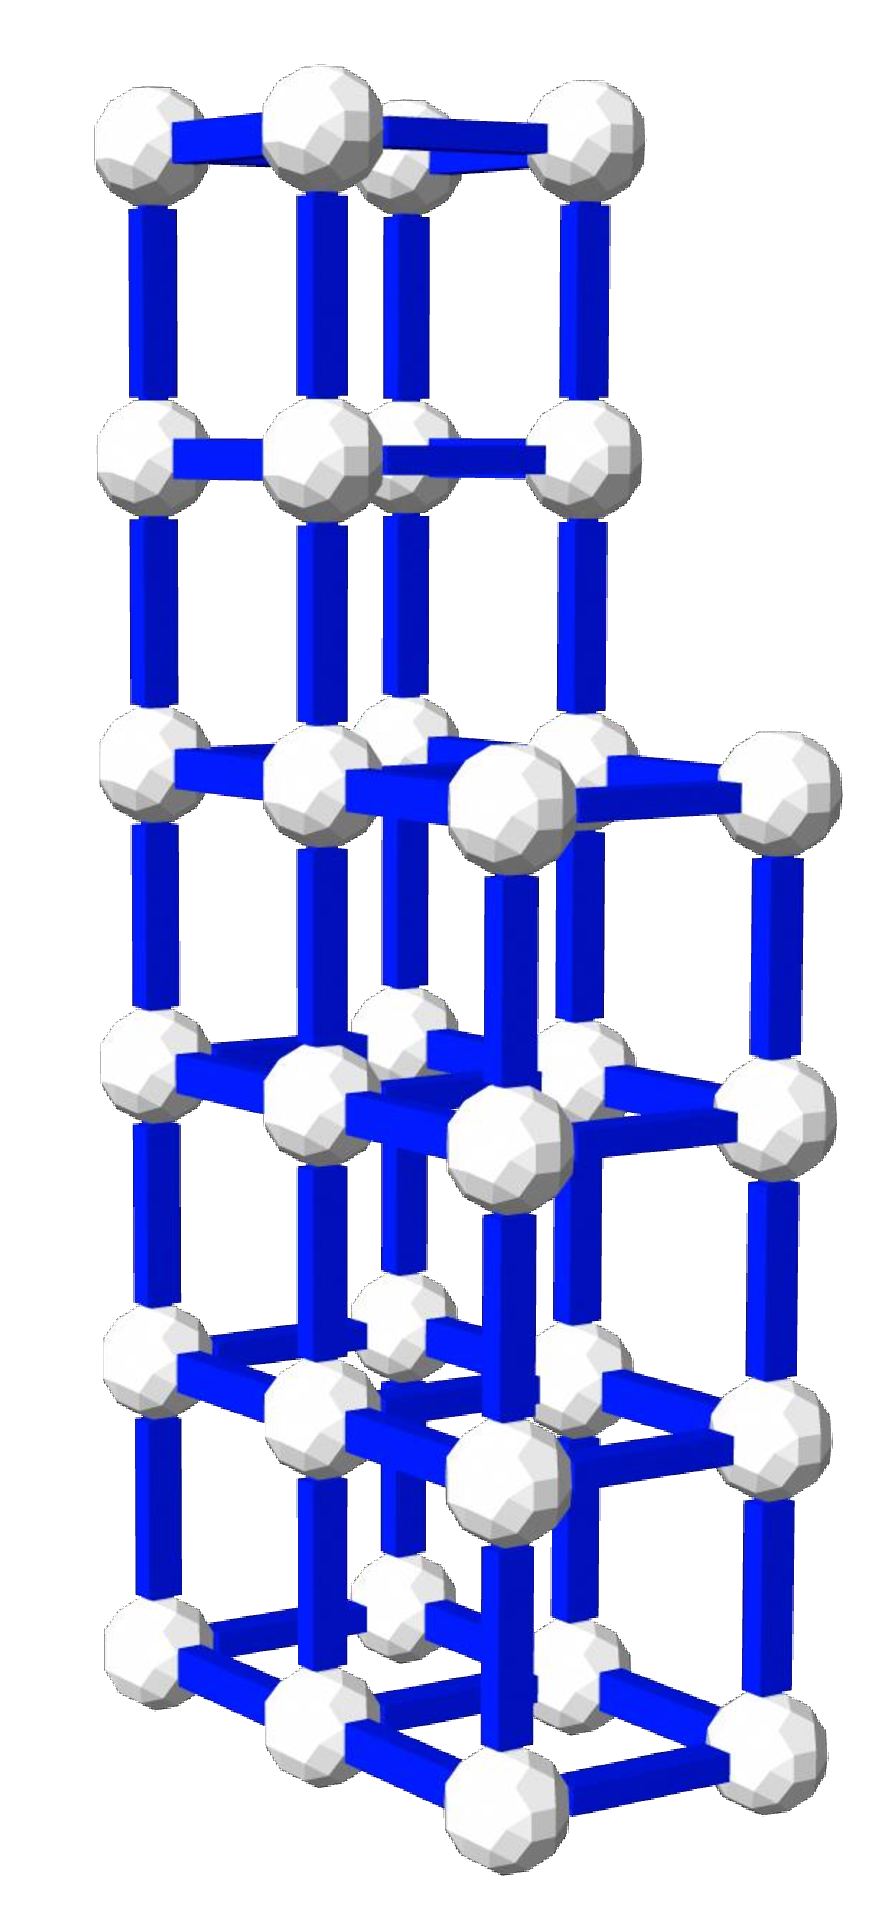
\includegraphics[width=0.1\textwidth]{figs/Zometool_init2.pdf}
% \caption{Initialize the Zometool structure with cubes}
\label{fig:Zometool_cont}
\end{wrapfigure}

\subsection{Initialization}
%We first partition $S$ into $m$ segments ($S=\{s_1, \cdots , s_m\}$) using Shape Diameter Function (SDF)~\cite{shapira:2008:consistent} and clustering implemented in CGAL~\cite{cgal}.
%First we want to fill the inner volume of each segment $s_i$.
%Although we can use some existing works~\cite{zimmer:2014:Zometool} to generate the inner Zometool structure, we intend to use structure that is composed of simple primitives because it's simplicity and easy-assembility.
%Follow Zimmer \cite{zimmer:2014:Zometool}, we choose to use cube as the basic primitive to initialize the filling.
%The initialized Zometool structure is denoted as 
%$\bar{\mathcal{Z}}=\{\mathcal{Z}_0,...,\mathcal{Z}_n\}$, 
%where $n$ is the number of segments with embedded Zome tools 
% We know the math model of Zometool and how it works in previous section, and decide the inner structure growing method. 
% The main feature of Zometool is let it can build thousands of structures. However, more complicated structure will take the more assembling time. 
Although we can assemble many complicated structures using Zometool, the assemble complexities and time consumption grows pretty fast as the number of Zometool items (rod and ball) used.
Our idea is that choosing the simple and repeated unit structure to make up the initial structure, and then growing out from main structure to get better fitting of outer surface. 
After experimenting different basic structure, such as cube, triangular pyramid, square-based pyramid and pentagonal pyramid, we choose cube as unit building block due to it's smallest assemble time.
% We find that triangular pyramid can get the best fitting but cube can get the less assembling time. 
% Finally, wants to approach our goal \textbf{fast assembling}. 
We follow Zimmer~\cite{zimmer:2014:Zometool} with cube as the basic unit to initialize the filling. 
The major difference from Zimmer~\cite{zimmer:2014:Zometool} is that we choose $b_0$ (the length of shortest blue rod) for our edge length of cube. 
The reason is that the smaller the cube is, the higher fitting rate we can achieve, and the inner structure will get closer to outer surface (see inset for sample initialization). 

%\section{Simulated annealing}
%After get the initial structure, the structure still too rough and weak for the inner structure. We want to more close to the outer structure and get more robust structure. But the main problem is thousand of possibility of Zometool. So we choose simulated annealing to make the problem be solved. The core of simulated annealing is design the (i) local operation, (ii) energy function and (iii) cooling schedule. The following context will discuss our design detail.


% \begin{wrapfigure}{r}{0.25\columnwidth} %this figure will be at the right
% 	\hspace{-5pt}
%   \begin{center}
%     \includegraphics[width=0.23\columnwidth]{figs/accuracyConstraints/accuracyConstraints.pdf}
%     \end{center}
%     \vspace{-5pt}
% \end{wrapfigure}

\subsection{Problem Formulation}
We measure the quality of the Zometool structure $\mathbf{Z}$ \ignore{model }with an energy $E$ which is composed of 4 terms according to different quality measurements:
\begin{align}
\label{eq:sa_energy}
E(\mathbf{Z})&=w_{\text{dist}}\cdot E_{\text{dist}}(\mathbf{Z}) + w_{\text{reg}} \cdot E_{\text{reg}}(\mathbf{Z}) \nonumber \\ 
&+ w_{\text{val}}\cdot E_{\text{val}}(\mathbf{Z}) + 
w_{\text{sim}} \cdot E_{\text{sim}}(\mathbf{Z}),
\end{align}
(we set $w_{{dist}}$ = 1.0, $w_{{reg}}$ = 100.0, $w_{{val}}$ = 1.0, $w_{{sim}}$ = 1.0 through all examples shown in this paper.)

\subsubsection{Distance}
The distance from $\mathbf{Z}$ to $S$ is integrated over all the nodes :
\begin{align}
E_{\text{dist}}(\mathbf{Z}) = \frac{1}{P\cdot d^2_{\text{norm}}} \sum_{i=1}^{P} \|p_i - \pi(p_i) \|^2 \cdot (1+F(p_i)),
\end{align}
where $P$ is the number of nodes and the normalization factor $d_{\text{norm}}$ is used to relate distance to the fixed length of the struts.
We follow \cite{zimmer:2014:Zometool} and define the term $F(p)$ called forbidden zone, which penalizes node points lying too far away from surface. 
%Please see ~\ref{forbidden} for more details.

\paragraph{Forbidden Zone}
% \note{Even if long distance from surface will cause the higher energy, we still want to accelerate the process.} 
During energy computation, the distance have to multiply the additional weight which is called Forbidden zones in \cite{zimmer:2014:Zometool}. 
$F(p)$ is defined as a quadratically increasing function which depends on the distance between the triangle centroid position $p$ to the nearest node $S$. $F(p)$ will be zero when the distance is smaller than $d_{\text{min}}$ and will be $F_{\text{max}}$ when the distance is larger than $d_{\text{max}}$. 
After a series of tests, finally we get the best parameters. 
We set $d_{\text{min}}$ = 16.0 ($\frac{1}{3}$ length of $b_0$) , $d_{\text{max}}$ = 47.3 (length of $b_0$) and $F_{\text{max}}$ = 70.0 for all the examples in this paper. 
%(see \figname~\ref{fig:forbidden})\label{forbidden}

% \begin{figure}[ht]
% \centering
% 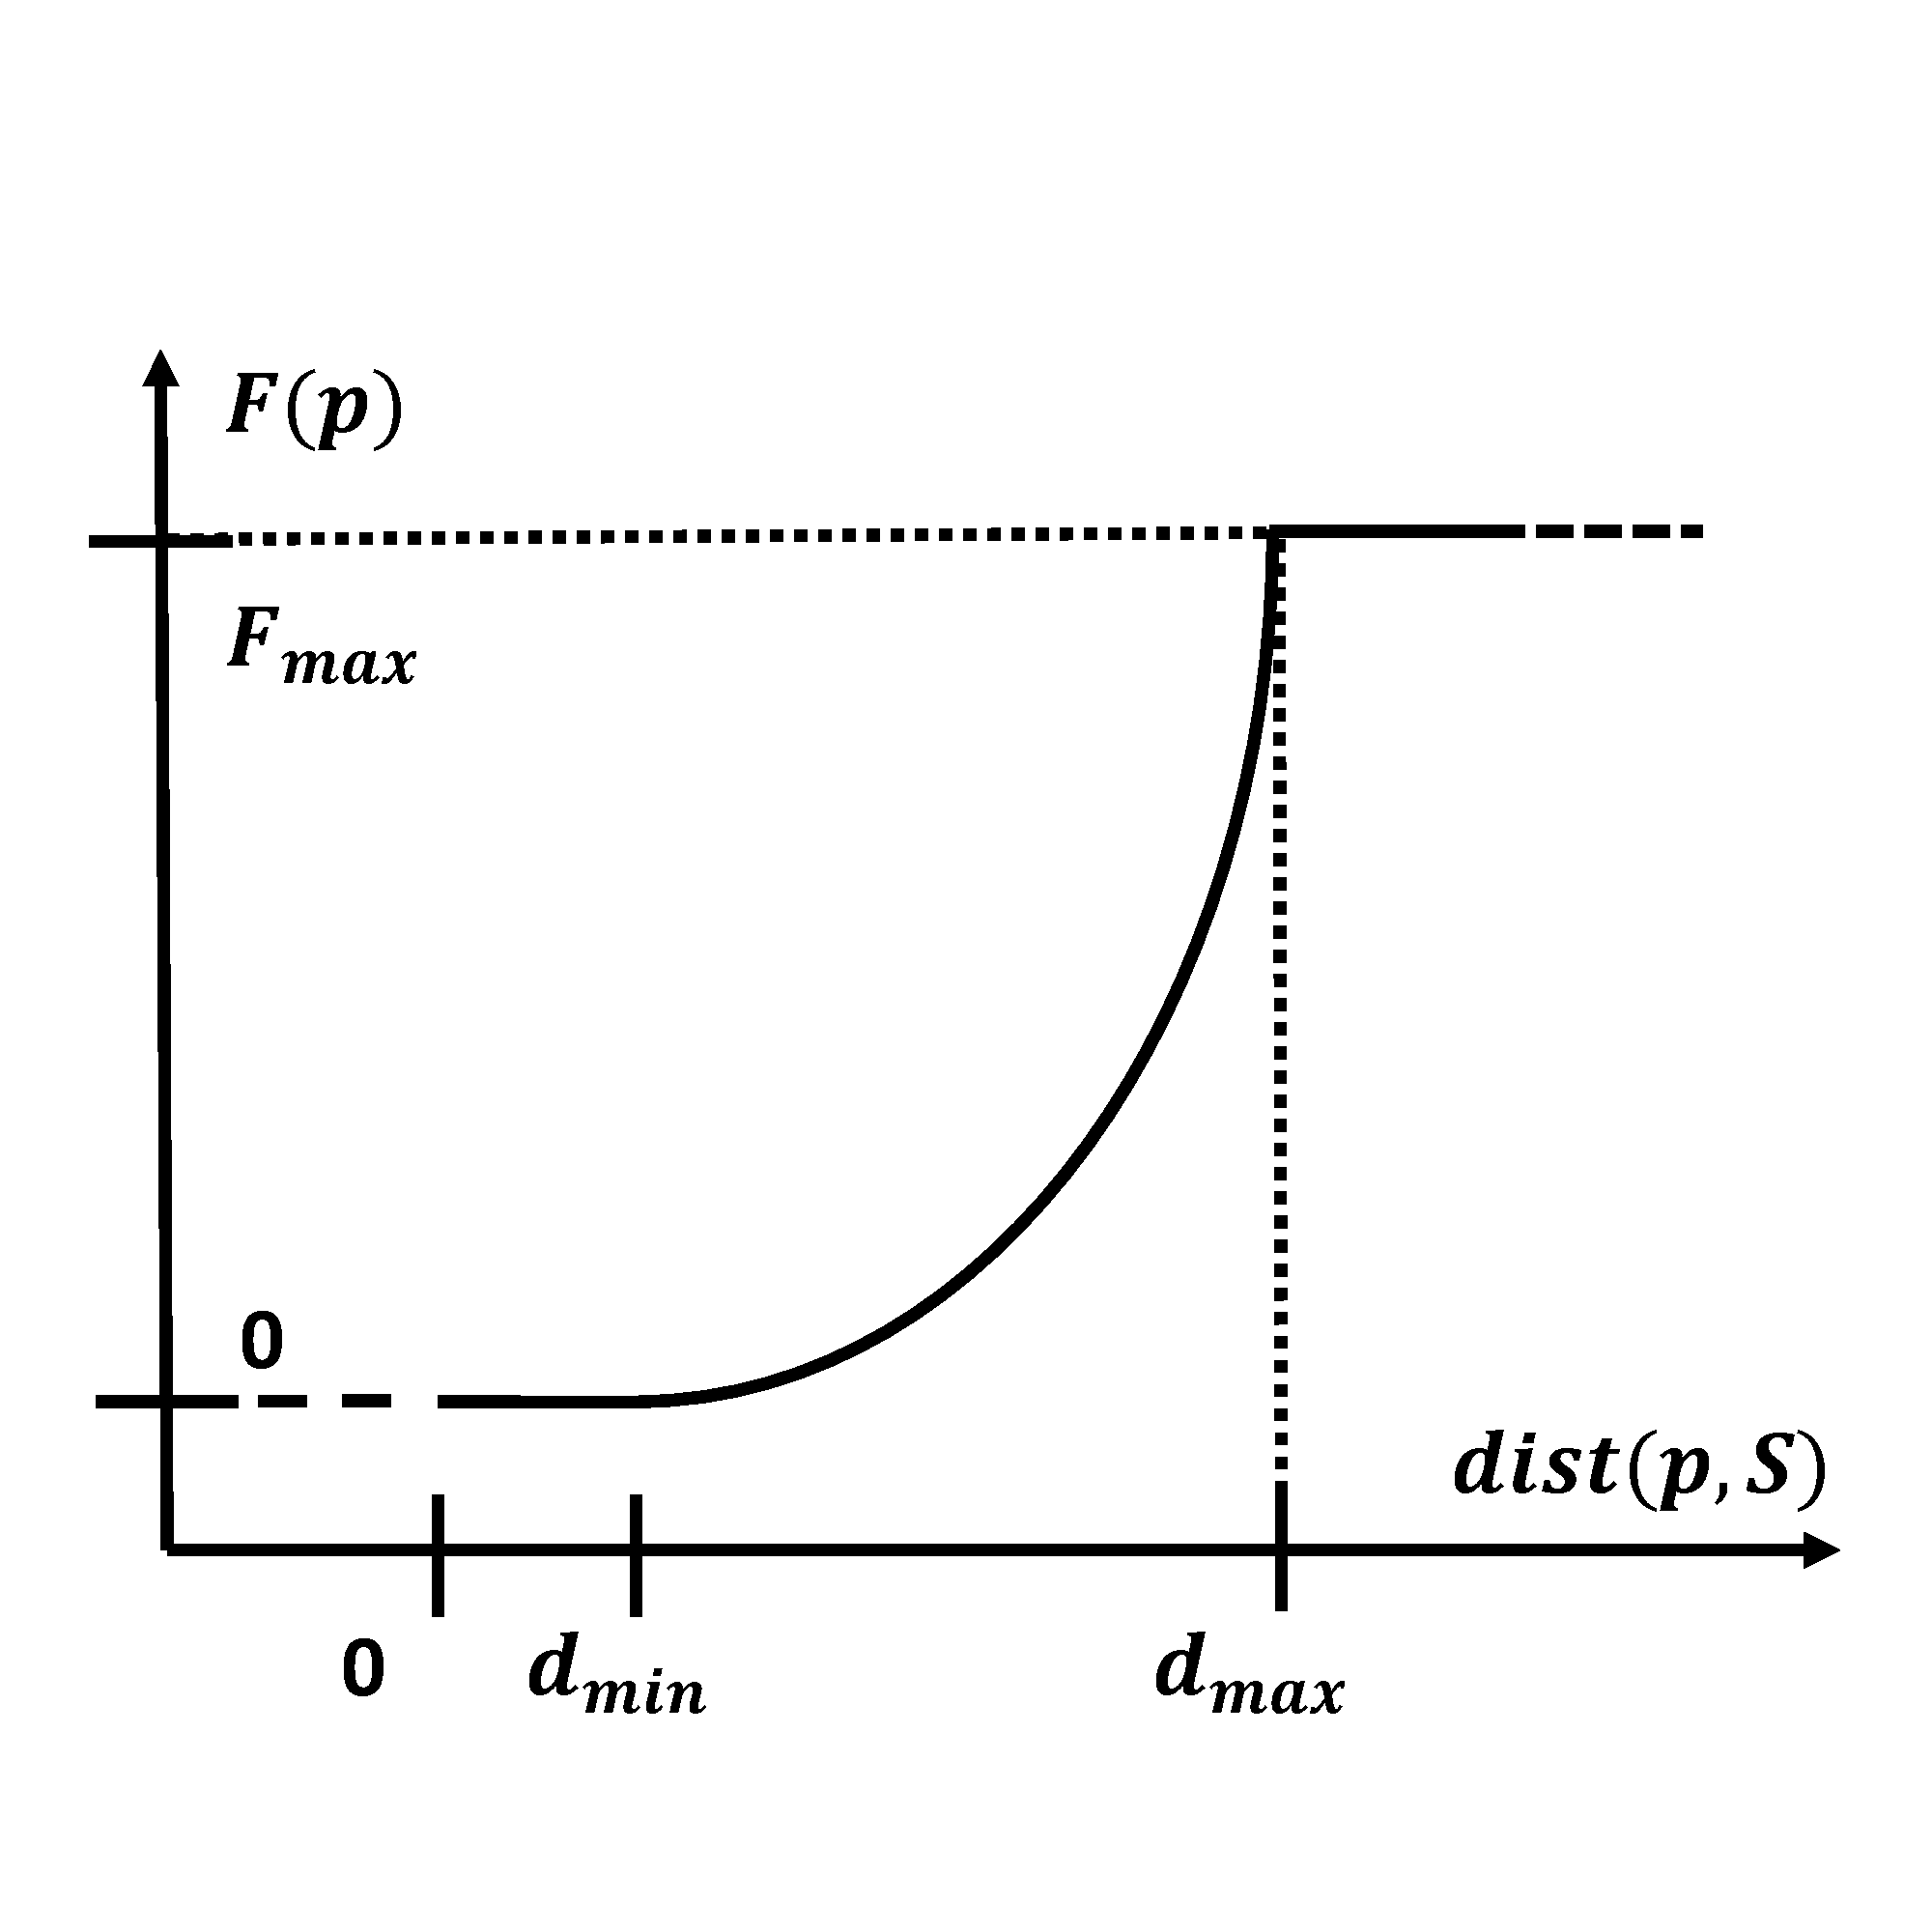
\includegraphics[width=1.0\linewidth]{figs/forbidden.pdf}
% \caption{Forbidden Zone}
% \label{fig:forbidden}
% \end{figure}

\subsubsection{Regularity}
In order to obtain a regular Zometool structure for simple assembling, we intend to regularize the angles between struts to be exact $90^\circ$ and penalize angle that is too small or too big (see \figname~\ref{fig:Regularity}).
% If the rods are too closer to each other, it is hard to construct them. 
% We hope the rods become discrete and the structure have suitable angle for construction. Hence, we set the baseline angle to $90^\circ$. This term will make our structure more regular.
\begin{align}
E_{\text{reg}}(\mathbf{Z}) = \frac{1}{|\mathcal{N}_i|} \sum_{p_j\in\mathcal{N}_i} (\text{min}(\theta_{ij})-\frac{\pi}{2}),
\end{align}
where $\mathcal{N}_i$ are the adjacent struts of strut $i$.

\begin{figure}[ht]
\centering
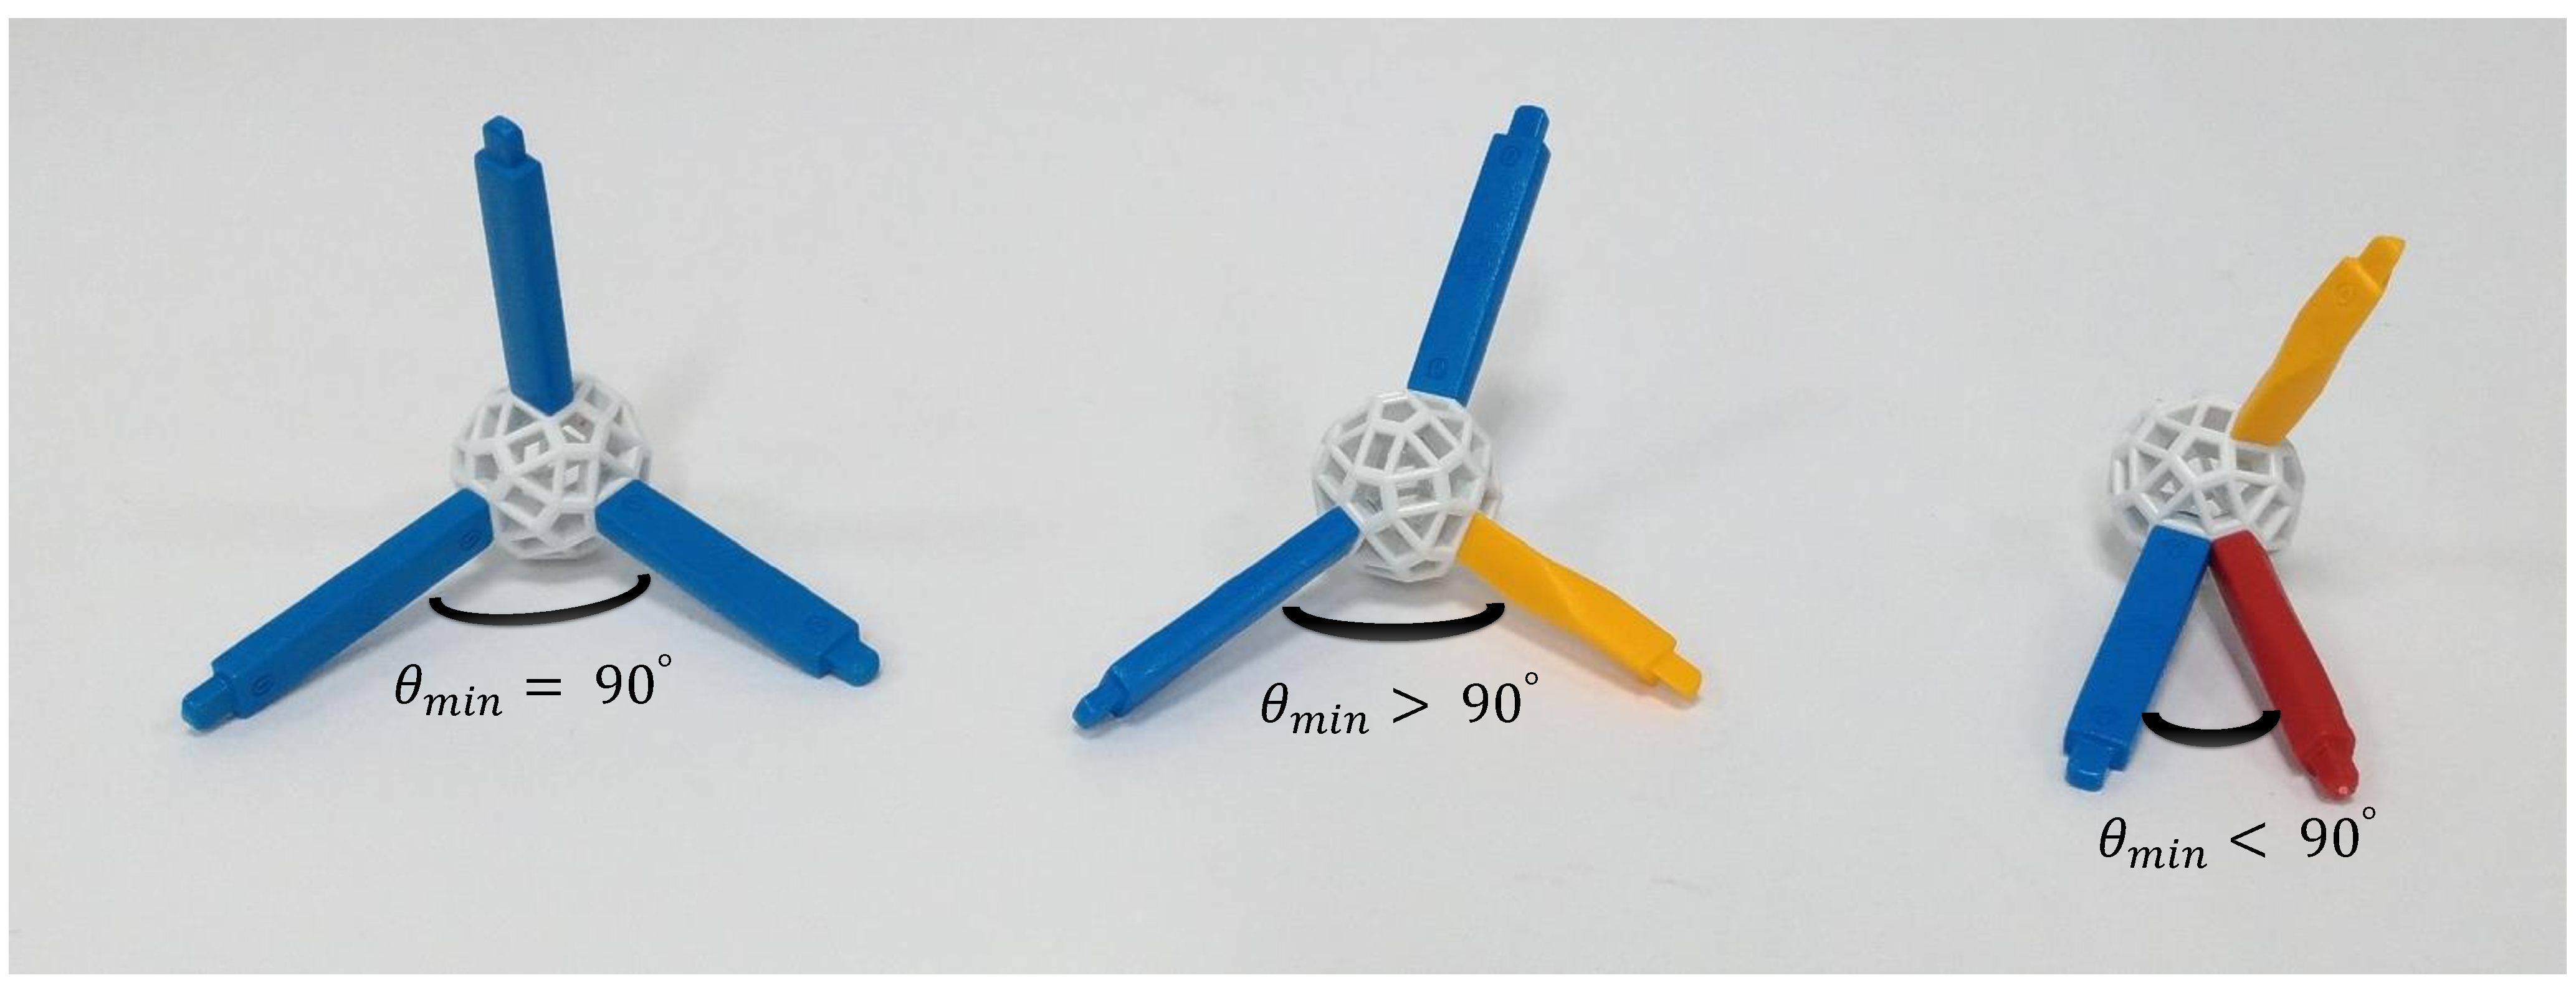
\includegraphics[width=1.0\linewidth]{figs/Regularity.pdf} 
\caption{\textbf{Regularity.} We penalize the configuration with minimum angle between struts smaller or greater than $90^\circ$.}
\label{fig:Regularity}
\end{figure}

\subsubsection{Valence}
We regularize the optimized Zometool structure to have a good valence for simple structure (see \figname~\ref{fig:Valence}). 
In order to maximize each Zome-ball's utility and minimize the complexity, we have to set a baseline number of rods as a constrain.
We set the target valence as $6$ from the initial cube structure.
\begin{align}
E_{\text{val}}(\mathbf{Z}) = \sum_{i=1}^{P} \frac{(V_p-6)^2}{6},
\end{align}
where $V_p$ is the valence of each node.

\begin{figure}[ht]
\centering
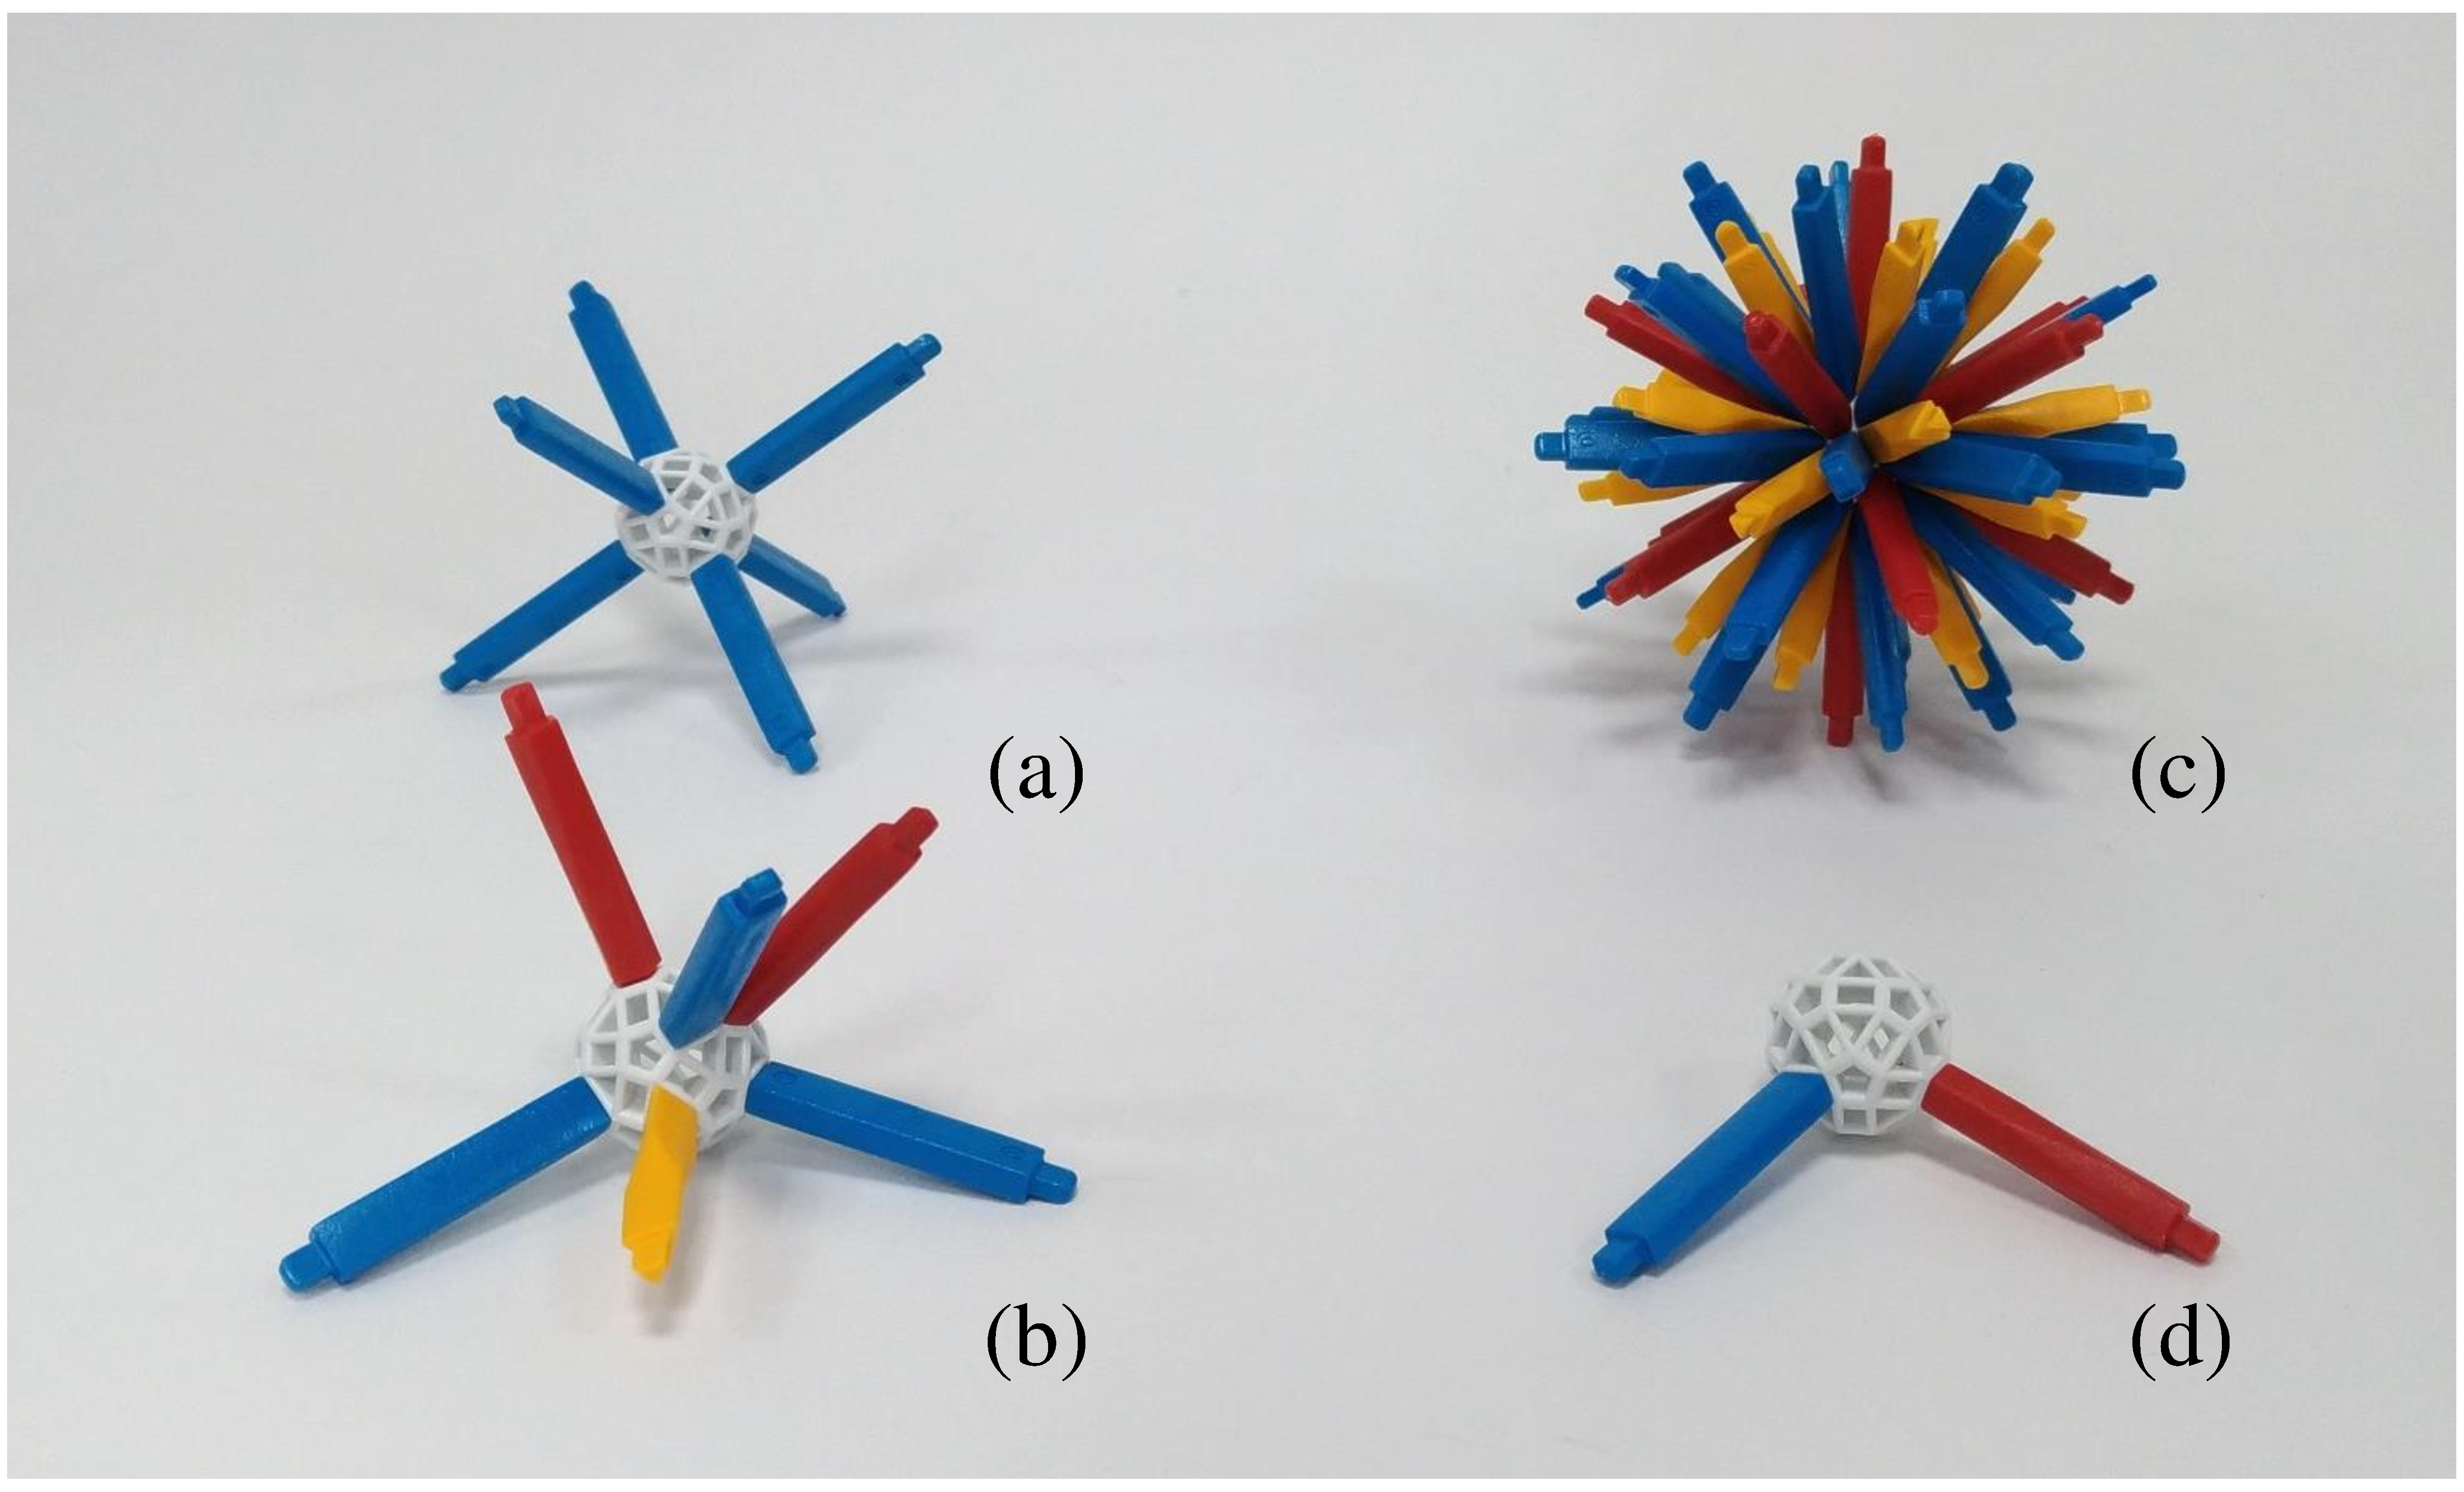
\includegraphics[width=1.0\linewidth]{figs/Valence.pdf} 
\caption{\textbf{Valence.} We encourage the valence of each Zometool node to be 6 (as in configuration (a) and (b)). 
We penalize the valence that is not 6 (configuration (c) and (d)).
}
\label{fig:Valence}
\end{figure}

\subsubsection{Simplicity}
Let $N$ is the total number of both nodes and struts, and $N_\text{target}$ be the target complexity.
The simplicity term is encoded as the quadratic differences from the target complexity:
\begin{align}
E_{\text{sim}}(\mathbf{Z}) = \frac{1}{N_{\text{target}}}(N-N_{\text{target}})^2,
\end{align}
% where $N$ is the total number of both nodes and rods.

\subsection{Exploration Mechanism}
% \ichao{Describe the process of Simulated Anealling}
Searching for the Zometool structure to minimize the energy $E(\mathbf{Z})$ (\eqname~\ref{eq:sa_energy}) is a non trivial optimization problem since $E(\mathbf{Z})$ is non convex and contains global terms. 
Exhaustive search is impractical and thus we adopt a more scalable strategy based on the Metropolis-Hastings algorithm \cite{hastings:1970:monte}.
In a nutshell, this algorithm makes a random exploration of the solution space by iteratively perturbing the current solution with a certain probability depending on the energy variation between the two solutions and a relaxation parameter $T$.
Following, we describe our local perturbation operators and relaxation scheme.
\algoname~\ref{alg:exploration} details the major steps of our optimization algorithm.

\begin{algorithm}[!ht]
\caption{Exploration mechanism}
\label{alg:exploration}
\begin{algorithmic}[1]
\Input{Initialized Zometools $\bar{\mathbf{Z}}$,\\ relaxation parameter $T=T_{init}$}
\Output{Optimized Zometoos $\mathbf{Z}$}
\Procedure{Exploration}{$\mathbf{Z}$}
\Repeat
    \State generate $\mathbf{Z}'$ from $\mathbf{Z}$ with a random local operation.
    \State draw a random value $p \in [0, 1]$ 
    % \State add the collision check here
    \If{$p < \text{exp}(\frac{E(\mathbf{Z})-E(\mathbf{Z}')}{T})$ and CollisionFree($\mathbf{Z}$)} 
        \State update $\mathbf{Z}' \leftarrow \mathbf{Z}$
    \EndIf
    \State Update $T \leftarrow C\times T$ \Comment{Update temperature.}
\Until{$T< T_{end}$}
\EndProcedure
\end{algorithmic}
\end{algorithm}

\subsubsection{Local Perturbation Operation}
During the exploration, we proposed four local perturbation operations (\figname~\ref{fig:local_op}) to construct the Zometool structure by minimizing \eqname~\ref{eq:sa_energy}.
\begin{description}[nosep,itemsep=0pt,leftmargin=0pt]
\item[Split] This operator insert a new node and  two rods to split the original rod.
\item[Merge] This operator insert a new rod to merge two disconnected nodes (two nodes can travel by two edges). 
\item[Bridge] This operator insert a new rod to merge two disconnected nodes (two nodes can't travel by two edges).
\item[Kill] This operator delete a node and two rods.
\end{description}

\begin{figure}[ht]
\centering
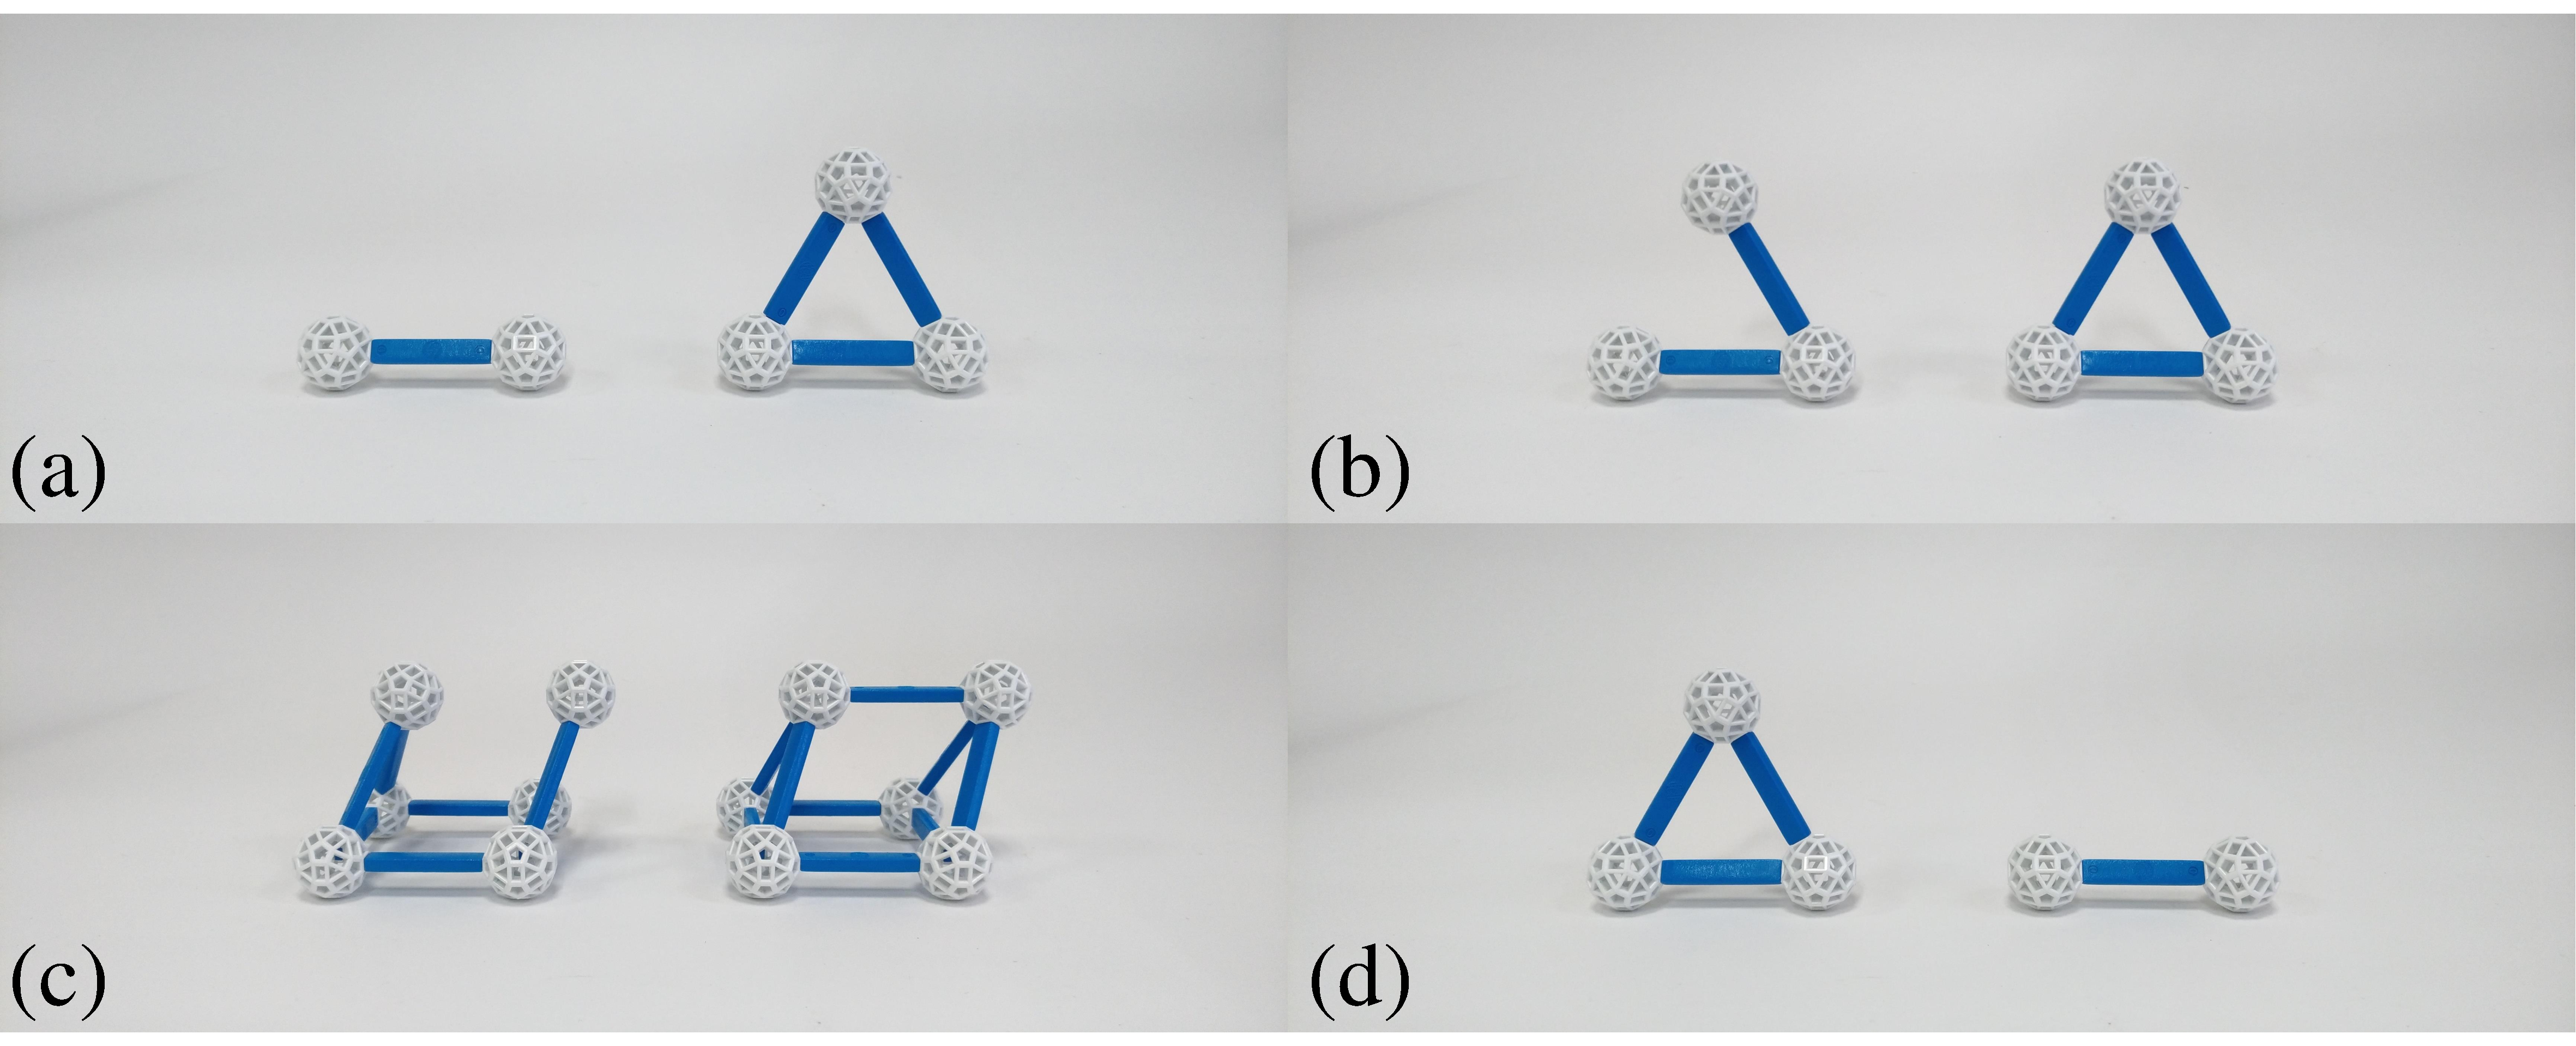
\includegraphics[width=1.0\linewidth]{figs/local_opt.pdf} 
% comment out first for faster compile
% 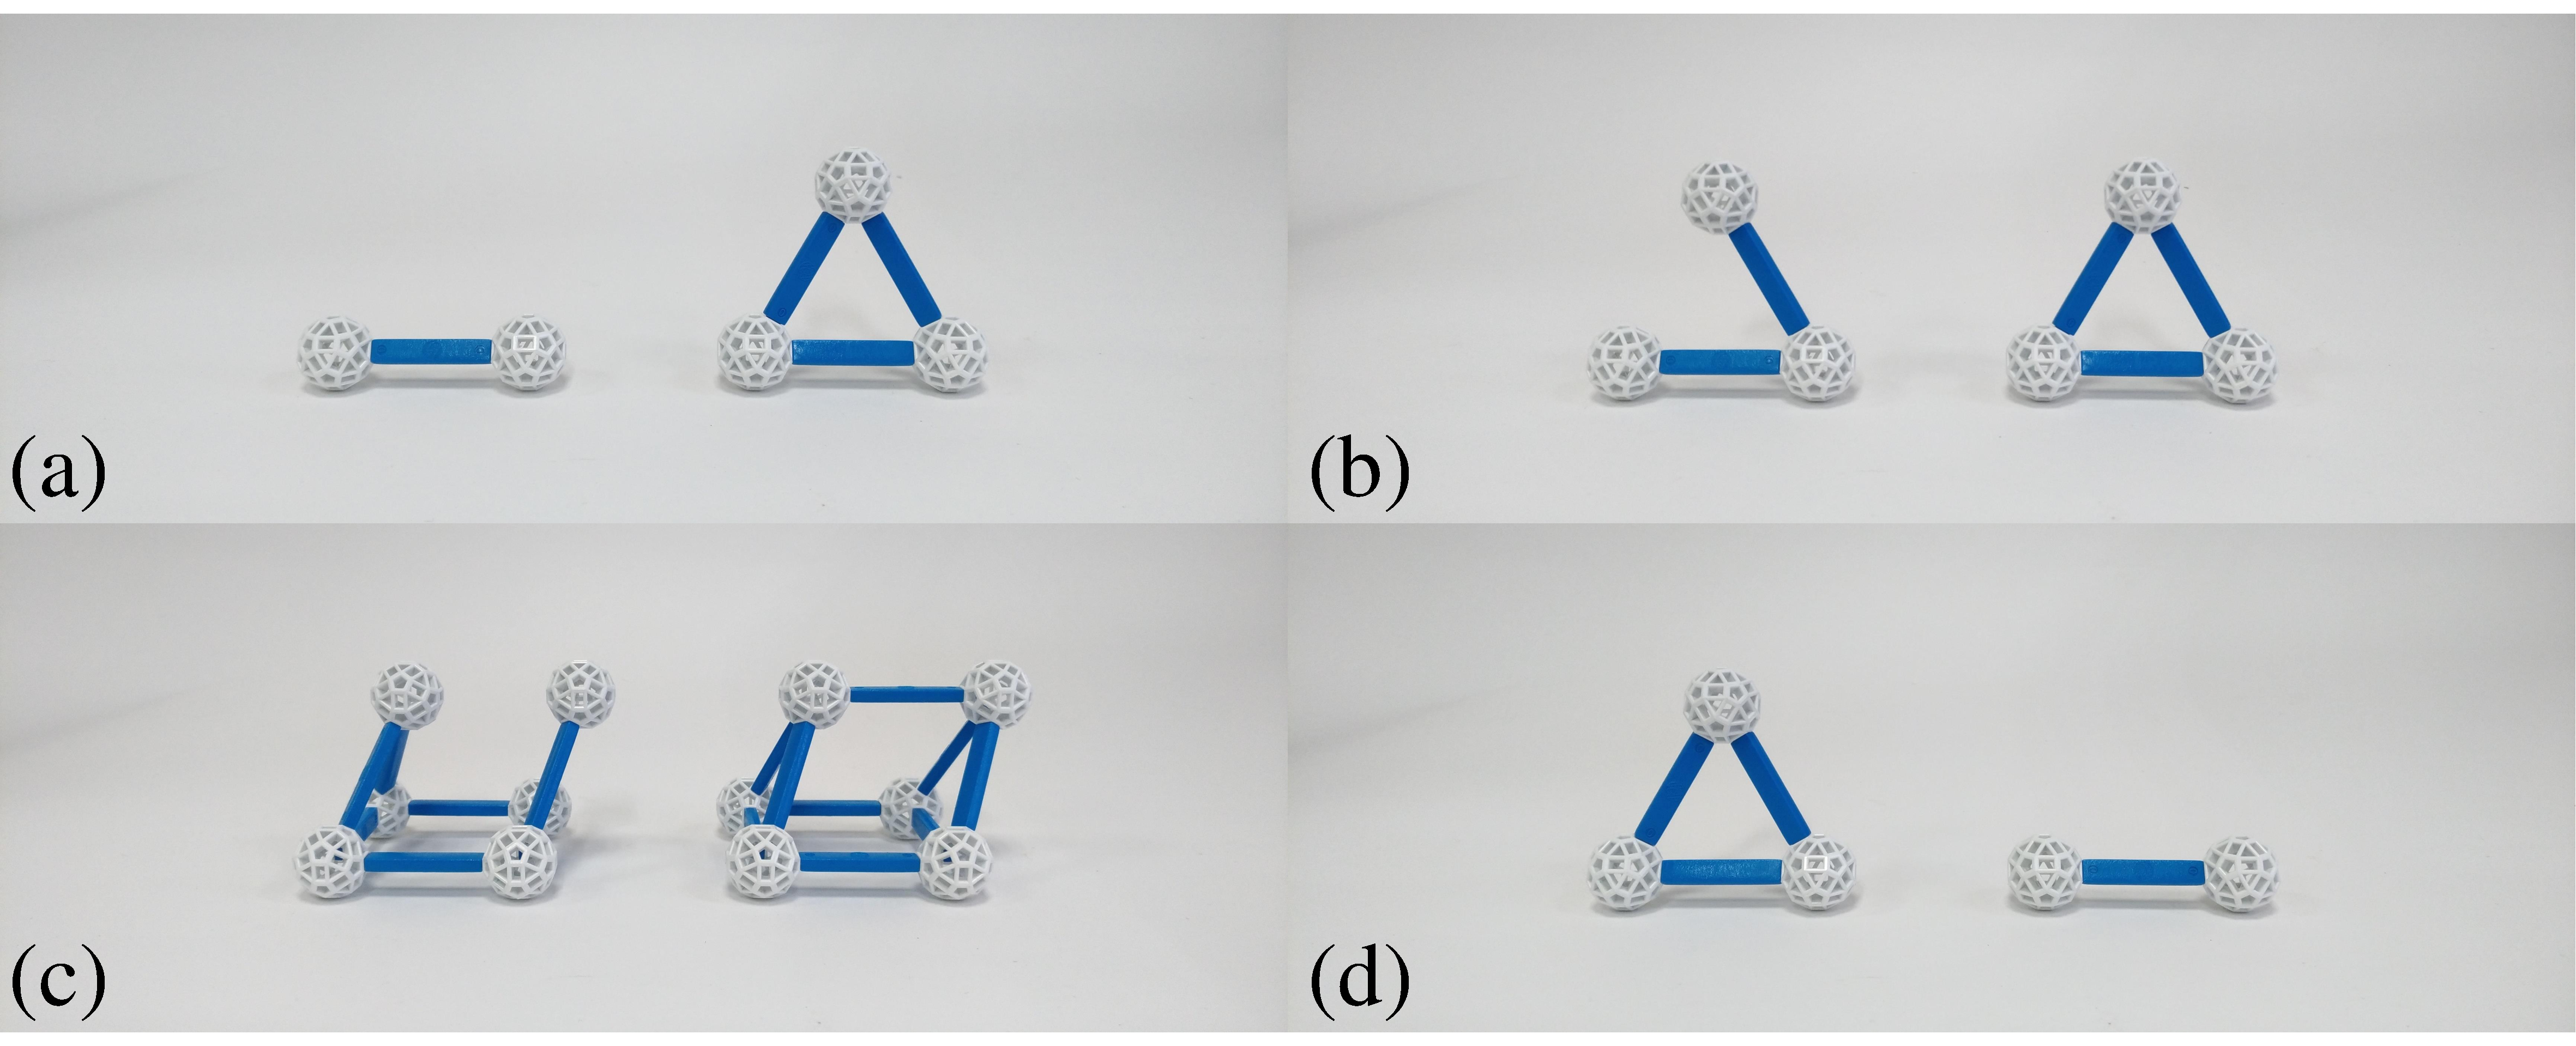
\includegraphics[width=\linewidth]{figs/local_opt.pdf} 
\caption{We use four local operations during structure perturbation. (a) Split, (b) Merge, (c) Bridge, and (d) Kill.}
\label{fig:local_op}
\end{figure}

\paragraph{Operation validity}
The operation will make the structure have some difference from previous round. However, not every round is valid. Our method of judgement which is collision detect is very simple. If the rods or Zome-ball get too close, the collision will happen and the structure will not be assembled. So this procedure will check whether the distance of Zome-ball to Zome-ball, rods to Zome-ball and rods to rods are too close.

\subsubsection{Cooling schedule}
% \ichao{Check what cooling schedule we used..}\\
The relaxation parameter $T$, referred as temperature, controls both the speed and the quality of exploration.
Start from initial temperature $T_{init}$, we decrease the temperature close to zero as iteration tends to infinity.
The decreasing process is referred as cooling, and different cooling schedules are exists for experiment.
Although the global minimum convergence is guaranteed using logarithmic cooling schedule~\cite{Salamon:2002:SA}, we rely on geometric cooling schedule~\cite{Henderson:2003:SA}. 
In our experiment, we set the initial temperature $T_\text{init} = 1$, and the decrease rate $C=0.99$ after every $100$ iterations.
\section{Object Partition}
\label{sec:surf_part}

\ichao{\figname~\ref{fig:nearest} and \figname~\ref{fig:cut_plane}} can be merged into one.

As mentioned in the beginning of this paper, most of the consumer-level 3D printers have limited printing volumes.
In order to print our large-scale object, it is necessary to decompose the object into different partitions.
Meanwhile, unlike traditional surface partition methods that only take surface features into consideration, we also need to consider the relationship between the outer surface partitions and the inner optimized Zometool structure.
More specifically, we will place connectors between the outer and inner structure in order to connect them (we will describe the design of the connector in more detail in~\secname~\ref{}).
% We aim to decompose the surface into different partitions for 3D printing
% with the optimized Zometool structure $\mathbf{Z}$ from \secname~\ref{sec:Zometool}.
Naively, we can simply compute the distance from each triangle $t$ to all the nodes in $\mathbf{Z}$, and assign $t$ to the nearest node as it's label.
However, inconsistency may arise among adjacent triangles, leading to unsatisfactory visual effects and assembly complexities (numerous small partitions might exist, see \figname~\ref{fig:nearest}). 
To address this issue, we formulate the problem as a multi-label graph cut minimization.
As each triangle $t$ can potentially correspond to different Zometool node, it gets assigned data cost for different corresponding nodes.
Given $n$ elements, $k$ labels and $n\cdot k$ costs, finding the minimum assignment is a combinatorial problem and typical NP-hard.
We employ Boykov~\cite{boykov:2004:experimental} to solve it.

After the partition, we further regularize the boundaries between pieces by performing a multi-class classification.
The major reason is that we seek smooth boundaries in order to ease the assembling process.
% we have to find the method which can separate different labels. 
% There are many partition methods we can choose. Because our result have to assemble, our segment can't have the sharp edges which may increase the assembling complexity. The planar-cut is our first choice. 
We follow Wang~\cite{wang2016improved} and use the Support Vector Machine (SVM)~\cite{cortes1995support} classifier to find our cut-plane. 
We will describe the detail formulation and implementation of MRF problem and how to find the cut planes in the following paragraph.
% The following context will describe more implementation details about graph cut and cut-plane.

\begin{figure}[ht]
\centering
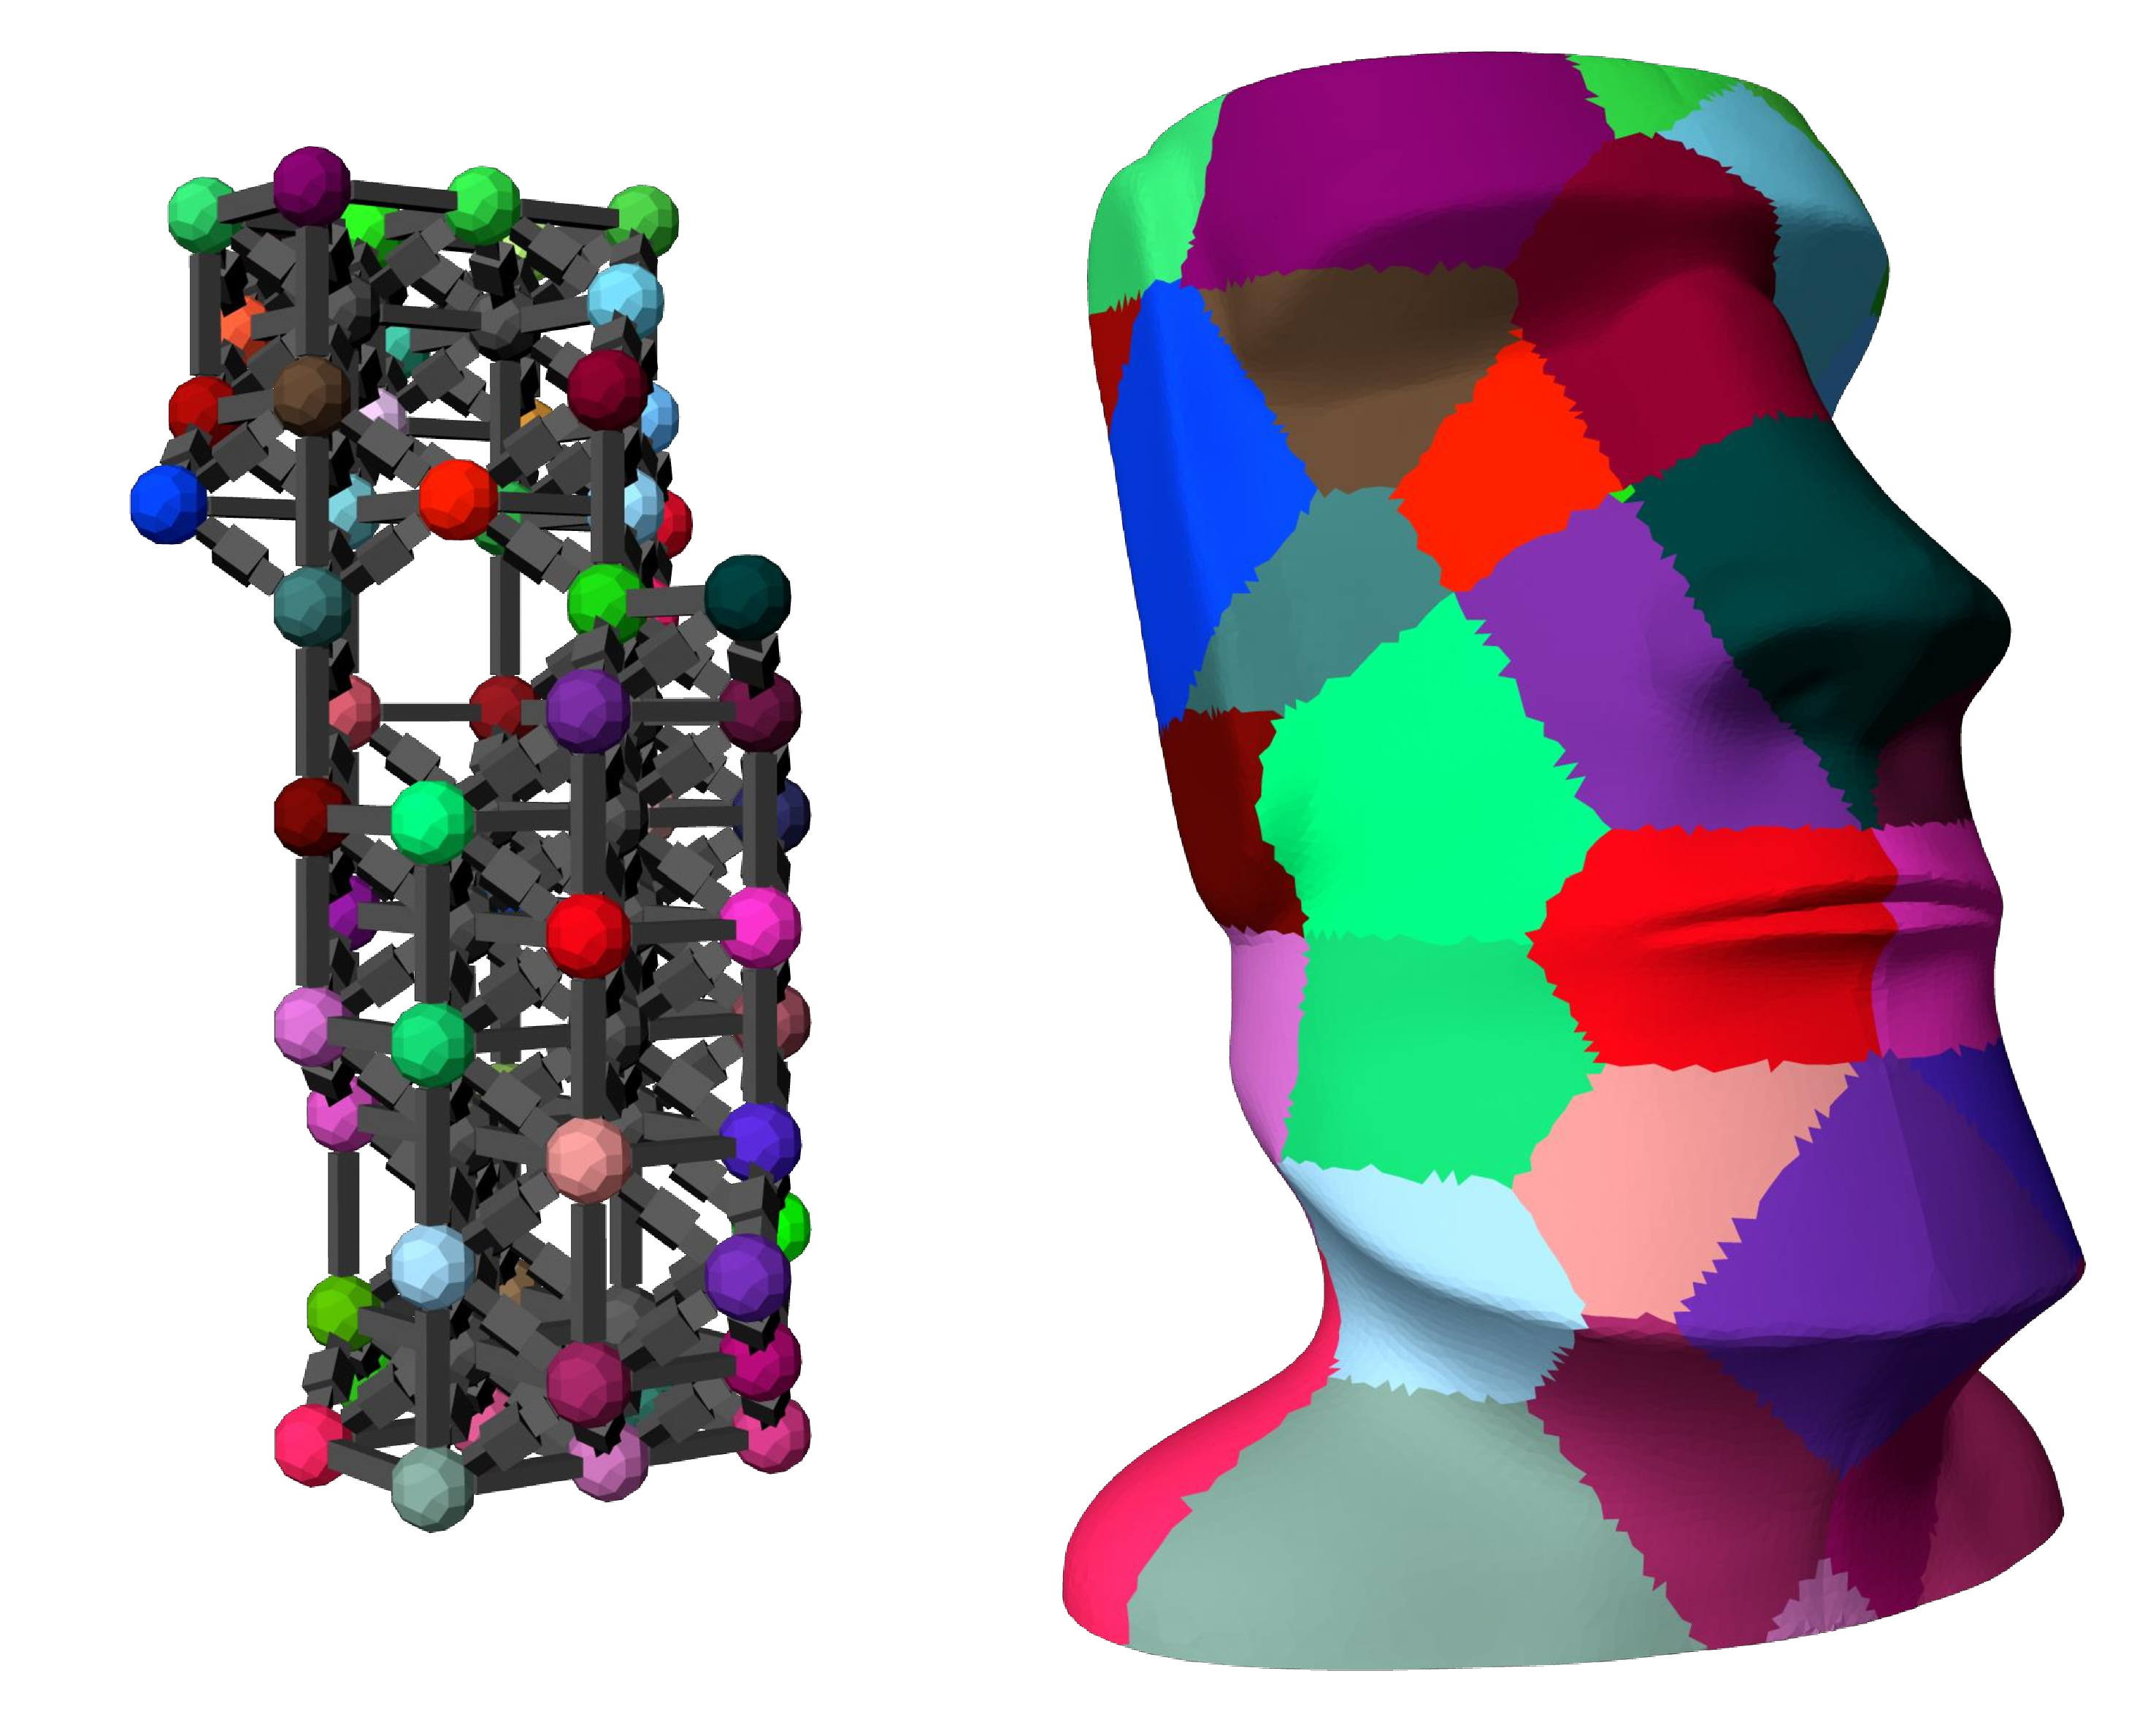
\includegraphics[width=0.75\linewidth]{figs/nearest_node.pdf} 
\caption{Simple classification. We assign each triangle to it's nearest node. But there are too many labels and some regions are too small for 3D printer to print it, So, we need to reclassify the result.}
\label{fig:nearest}
\end{figure}

\subsection{Surface Partition}
\paragraph{Optimization energy}
We compute the assignment function $f$ that assign label to each triangle $t$, where $t \in T$, such that the labeling $f$ minimize the following energy $E(f)$:
\begin{align} \label{eq:graph}
E(f) = w_{data} * \sum_{t\in T}D(t, f_t) + w_{smoothness} * \sum_{t,s\in N} S(t, s, f_t, f_s),
\end{align}
and we optimize this function using multi-label graph-cut algorithm proposed by Boykov~\cite{boykov:2004:experimental}.
In our setting, the entire outer nodes of $\mathcal{Z}$ are complete possible label set $L$.
This $E(f)$ consists of two separate terms, i.e. data and smoothness.
Next, we will explain each term in more detail.

\subsubsection{Data cost}
Data cost measures how well a triangle $t$ covers a node $p \in P$.
This cost is simply defined as the distance of the nearest node to the triangle.
\begin{align}
D(t, f_t) = -\omega \log(\mathcal{P}(p | t)),
% D(p,f_p) = \displaystyle\min_{p \in P}(d(t, p))
\end{align}
where $\mathcal{P}(p | t)$ is the probability of that triangle $t$ belong to the node label $p$, and $\omega$ is a constant that
regulates the influence of the data term in the total energy.
Here, we simply define $\mathcal{P}(p | t)$ as $1/d(t,p)$, where $d(t,p)$ is the distance of the node to the triangle.
\subsubsection{Smoothness cost}
Smoothness term measures the spatial consistency of neighboring elements.
\begin{align}
S(t, s, l_t, l_s) = 
\begin{cases}
0, & \text{if } l_t = l_s, \\
-\log(\theta_{t,s}/\pi)\varphi_{t,s} + w_{saliency} * E_{saliency}(t), & \text{otherwise} 
\end{cases}
\end{align}
where $\theta_{p,q}$ and $\varphi_{p,q}$ are the dihedral angle and distance between triangle $p$ and $q$, respectively.
With the smoothness term, two adjacent triangles are likely to have consistent labels.

\paragraph{User-guided saliency} 
We observed that there are many salient regions on each of the object we used, e.g. we don't want the partition seam to go through the eyes and nose on the face~\figname~\ref{fig:saliency}.
In order to preserve the salient region, we ask users to draw the region he thinks it's important to preserve, and we formulate this as part of the smoothness cost, which prevent the partition seam to cut through salient region~\figname~\ref{fig:saliency}.
% Every mesh have some features, such as eyes, nose or other unique objects. 
% But we can't get the feature information by only use relation of adjacent triangles. 
% If we don't assign some information during process of graph cut, the result just like left of \figname~\ref{fig:saliency}, the mouth and nose will be split in later process. Our saliency information is given by user guidance. For example (see middle of \figname~\ref{fig:saliency}), the user think the mouse and the nose is the important feature on mesh, so mark those parts and hope the parts don't be split in later process. Since we give the saliency information, the marked regions usually assign in the same part and prevent the slice seam on those regions.

\begin{align}
E_{saliency}(t) = 
\begin{cases}
1, & \text{triangle is marked as salient region}, \\
0, & \text{otherwise} 
\end{cases}
\end{align}

\begin{figure}[ht]
\centering
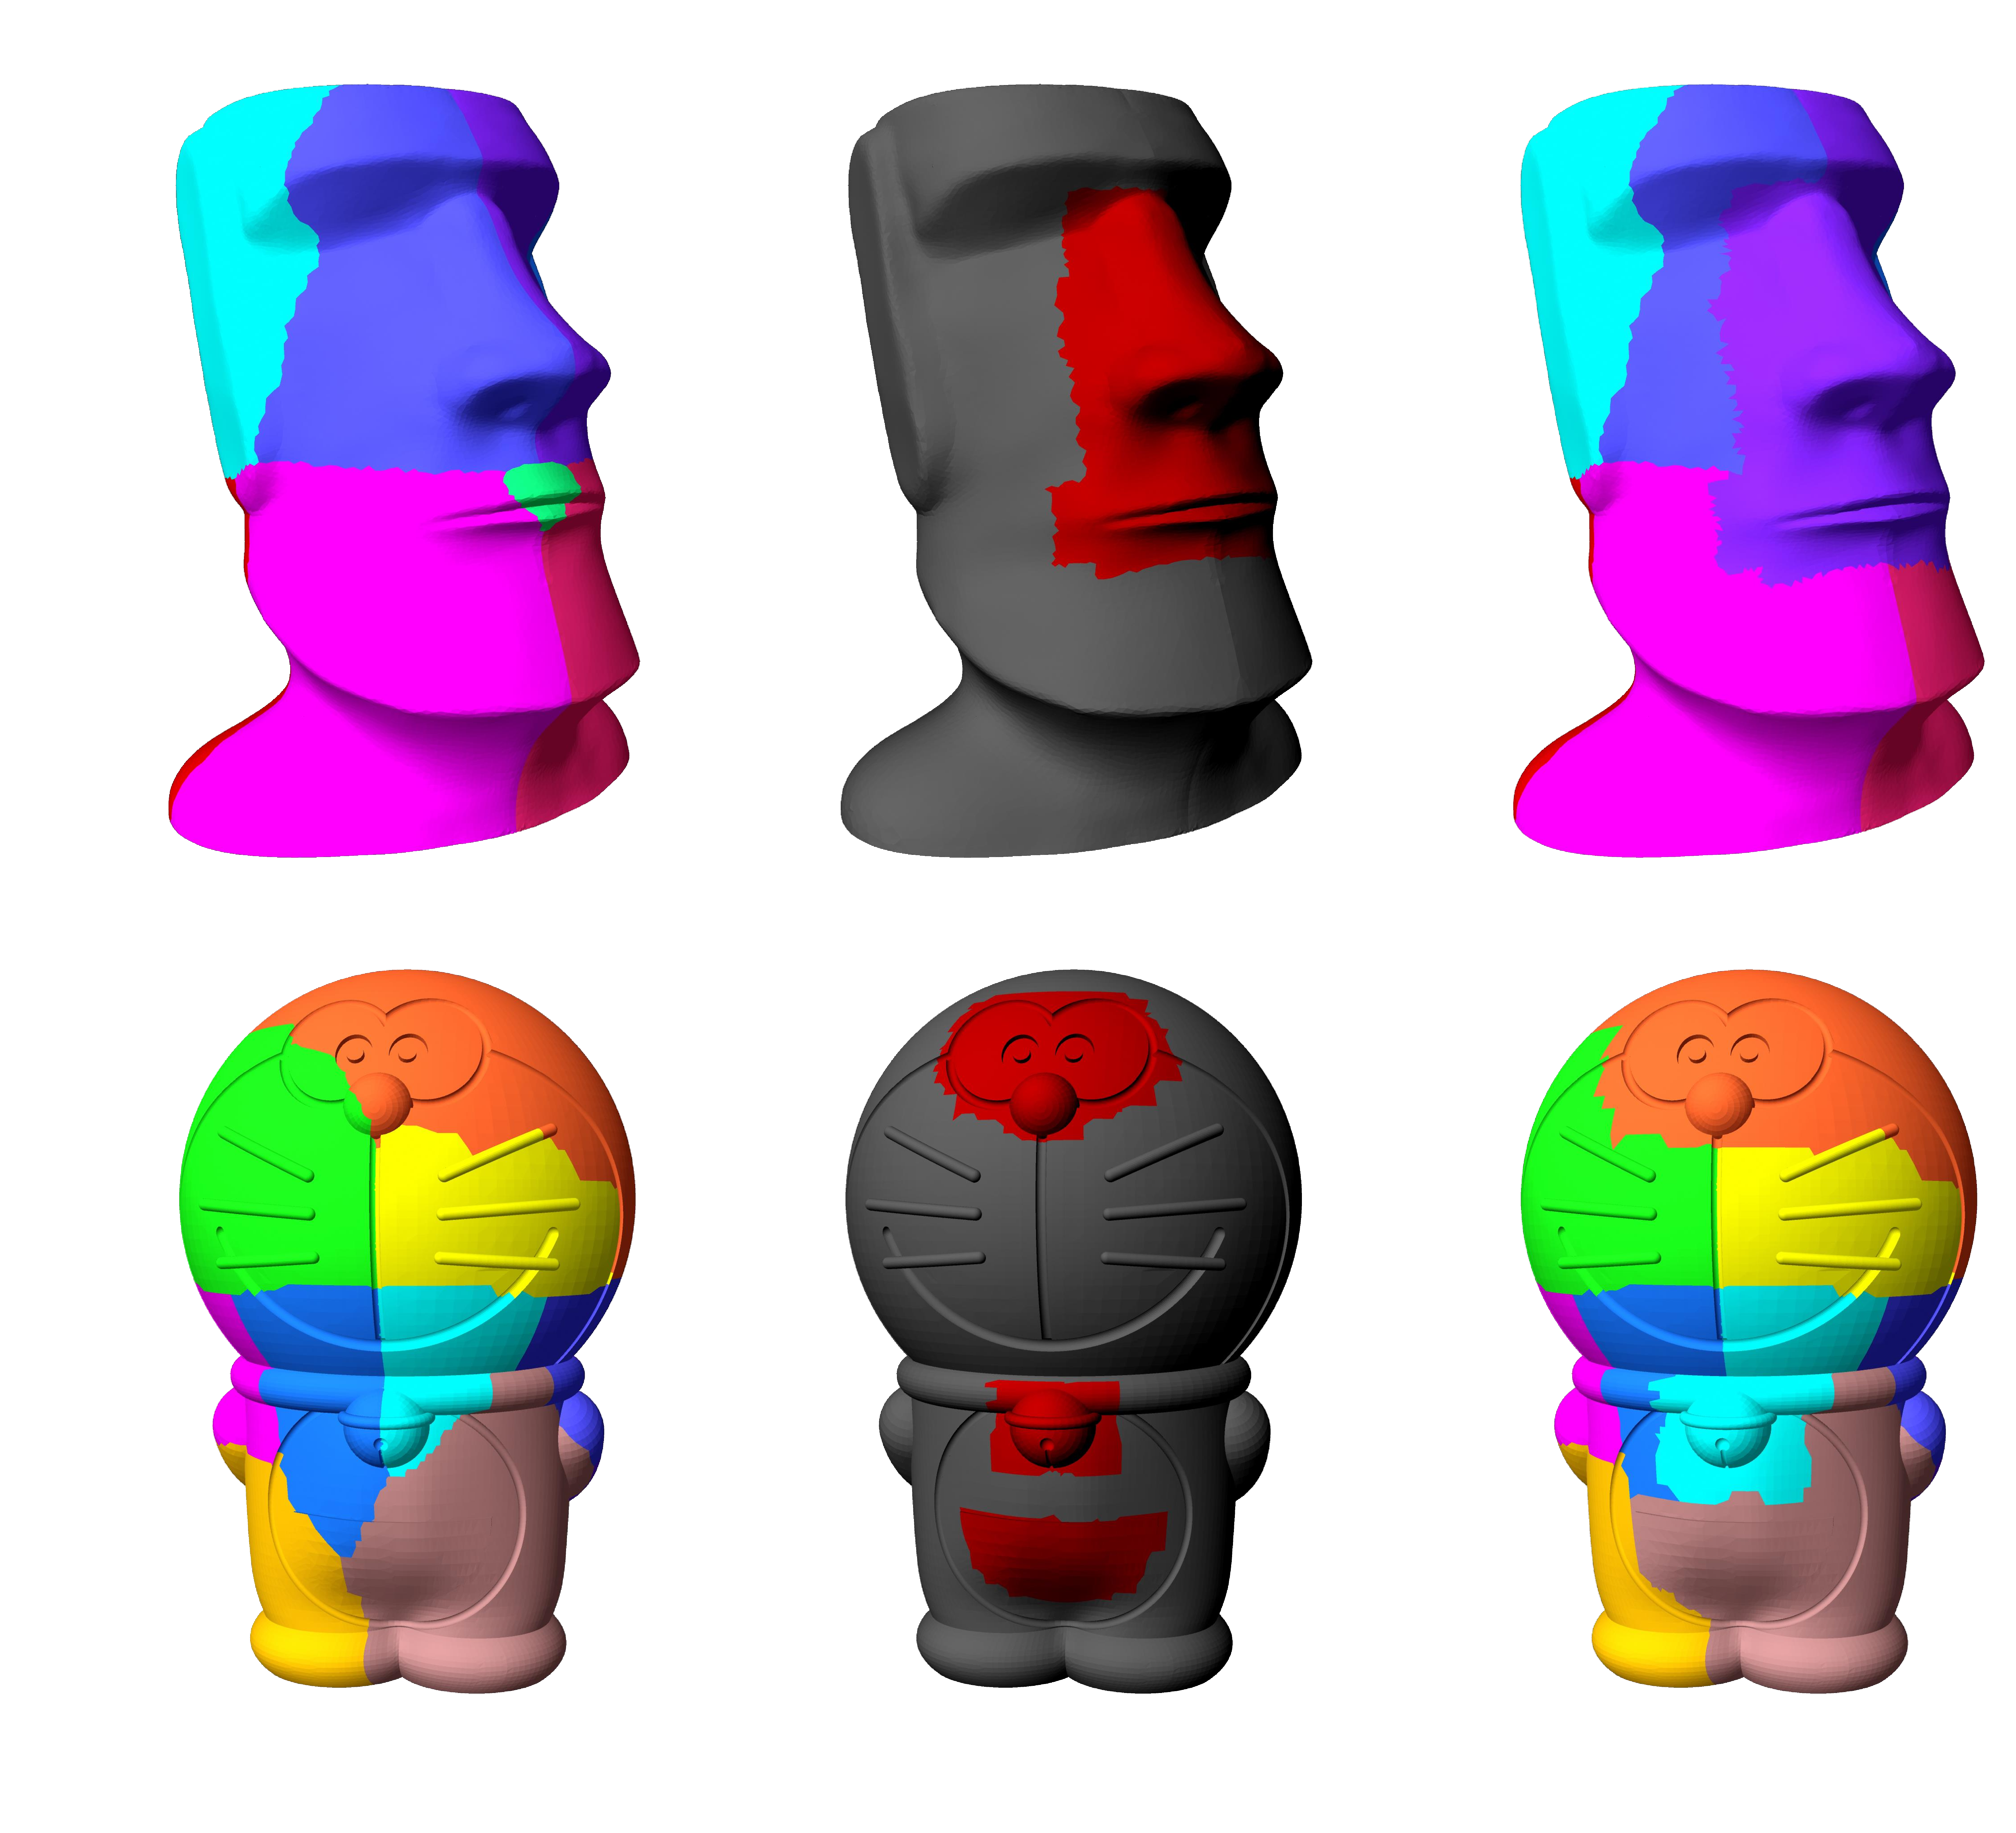
\includegraphics[width=1.0\linewidth]{figs/saliency.pdf} 
\caption{User-guided saliency. 
Origin result of graph cut may split some feature on the mesh. (Left of the figure) In order to solve it, we ask user to mark the unique feature. (Red region in the middle of the figure) We add those information for graph cut, and precent those regions from separating into multiple parts. (Right of the figure)} 
\label{fig:saliency}
\end{figure}

\subsubsection{Our result}
We solve the labeling problem~\eqname~\ref{eq:graph} with graph-cut and obtain 11 labels on the Maoi head object~\figname~\ref{fig:cut_plane}(a).
Compare to the naive method (\figname~\ref{fig:nearest}), we obtain smaller partition numbers (11 v.s. 60), and each of them are with better shape and size.
% Each label has better shape and size than that before reclassification. (See \figname~\ref{fig:cut_plane}(a)) Then, we have to separate each label into pieces for 3{D} printing.
% Before the labeling optimization, there are too many labels (60 labels in \figname~\ref{fig:nearest}) and some labels are too small. 
% By optimizing~\eqname~\ref{eq:mrf},
% Therefore, we use graph cut algorithm to optimize the energy function (Equation \ref{eq:graph}) which we design the data and smoothness cost. After the optimization, we get the result which has 11 labels. Each label has better shape and size than that before reclassification. (See \figname~\ref{fig:cut_plane}(a)) Then, we have to separate each label into pieces for 3{D} printing.

\subsection{Object Cut}
% There are many methods for mesh segmentation. The simple method is collecting all triangles of graph cut label, but it will cause the sharp edge. 
In order to cut the physical object into pieces, we have to find the cut planes that separate the space occupied by the object.
However, the boundaries between optimized partitions from previous step is not regularized enough for directly used as the separating plane. 
% For easy assembling, we have to split the triangles and regularize the contact surface between different labels. 
% We choose the planar cut for our method.
It is very difficult to find a plane in 3{D} space because of the varied plane normal vectors.
In order to obtain the desired cut planes, we analogize our problem to finding the separating plane in solving multi-class classification using Support Vector Machine (SVM).
We use each triangle as a data sample, with it's location as feature vector and the optimized label from previous step as it's class.
In short, SVM algorithm intend to find the best hyperplane which is the one that represents the largest separation, or margin, between the two adjacent classes. 
And we use the obtained hyperplanes from SVM as our cut planes (\figname~\ref{fig:cut_plane}(b)).

% We use the SVM classifier to generate the cut-plane. The different label of vertex is our input for training. Then, we can get the hyperplane which will separate different labels of data. But we don't have to know the hyperplane which separate the nonadjacent labels. So before we start training, we find the neighbor pair and use the information that can let us know which hyperplane needs for split the label.  By collecting all the hyperplanes, like \figname~\ref{fig:cut_plane}, we can use those planes for segmentation.

\begin{figure}[ht]
\centering
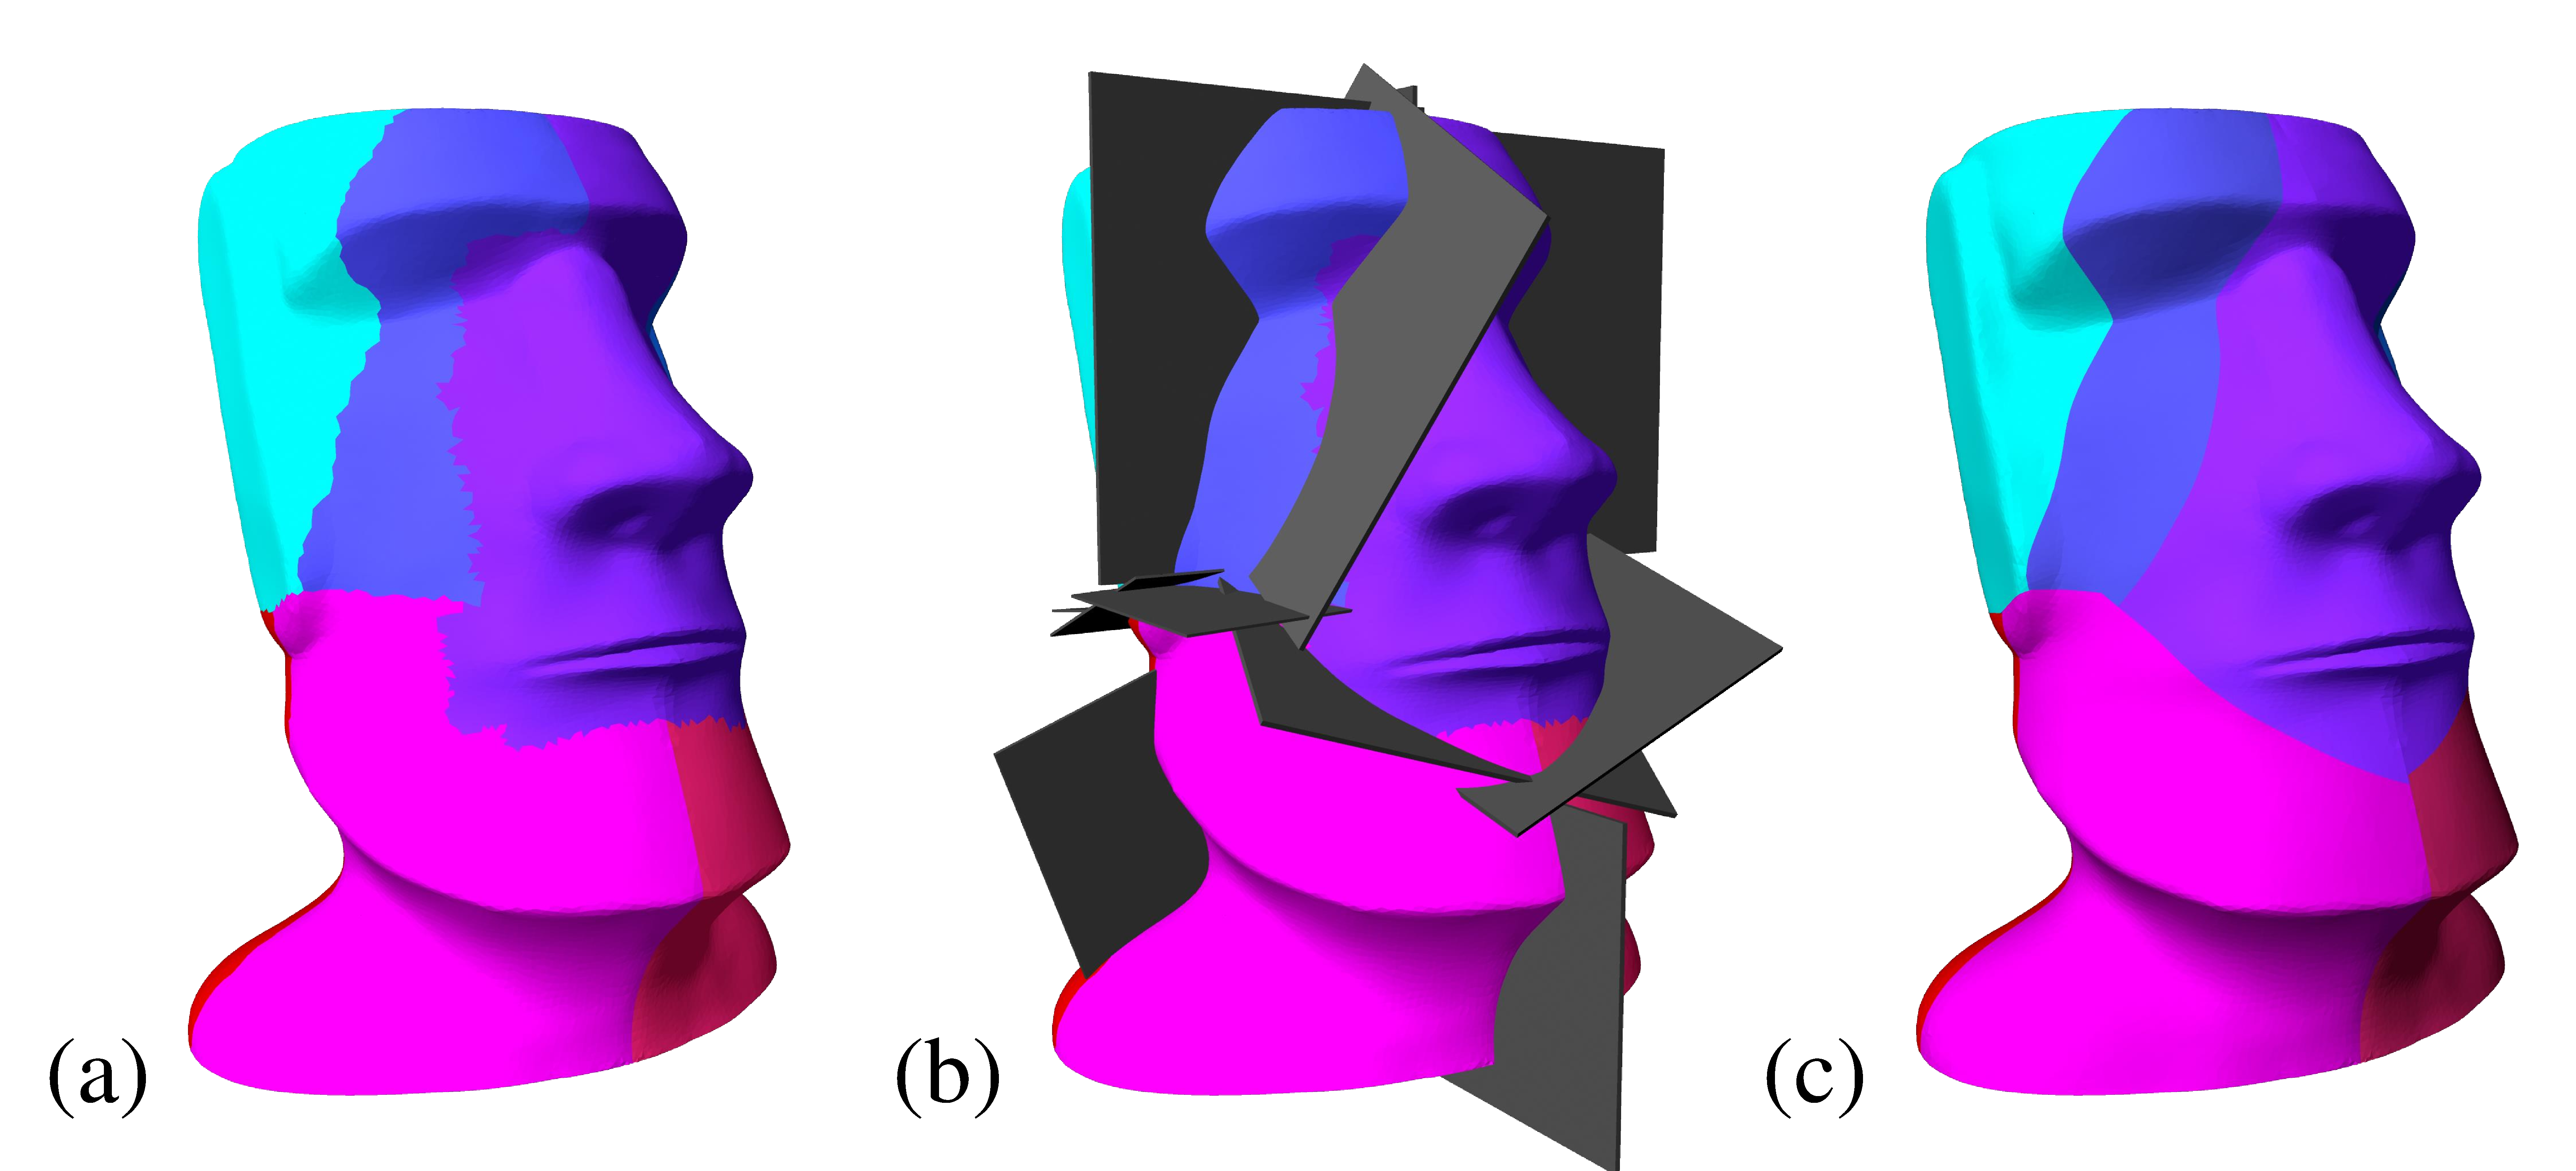
\includegraphics[width=1.0\linewidth]{figs/cut_plane1.pdf} 
\caption{(a) Result of graph cut (b) Cut-plane generated by SVM classifier (c) Cutting result} 
\label{fig:cut_plane}
\end{figure}


\section{Fabrication}
\label{sec:fab}
\chinky{Chi: here need some discussion.}
The object to be printed should be solid \chinky{mesh}\chireplace{, i.e. we have to fill in the inner space of the object with materials as well.}{.}
In our method, we use the Zometool structure to fill in most of the inner spaces, while still retaining \chinky{the} minimum thickness of the outer shell  \chireplace{due to the common setting of 3D printers.}{to form the input shape. The minimum thickness is defined due to the common setting of 3D printers.}
% Note that the thickness might change across different 3D printers.
% However, the input mesh just have the outer surface, and the valid pieces will have both outer and inner surface for 3{D} printer. 
% After we have the inner surface, the pieces have to connect to the Zometool structure. After the process we can get all pieces let can be fabricated, and then we assemble them by connecting to the optimized Zometool structure.
% In order to generate fabricatable shape, it is practical to leave a minimum thickness of the outer shell, and this thickness differs from each printer.
Thus, we prepare \chireplace{object}{segmented solid meshes} to be fabricated by generating \chireplace{a inner surface}{pieces} with a predefined thickness, and attach connectors on \chireplace{this inner surface to combine the inner and outer structure.}{those pieces to combine the Zometool structure.}
% and the remaining operations are performed within this inner surface.
    
\subsection{Inner surface}
\chinky{To construct the solid mesh as the outer shell, we need to obtain the inner surface and use the original surface as the outer surface.}
There are many potential ways to generate \chinky{the} inner surface. 
The simplest method is that shrinking the mesh along the vertex normals.
However, it sometimes generate\chinky{s} the surface with flipped triangles that stick out of the outer surface.

% \begin{figure}[ht]
% \centering
% 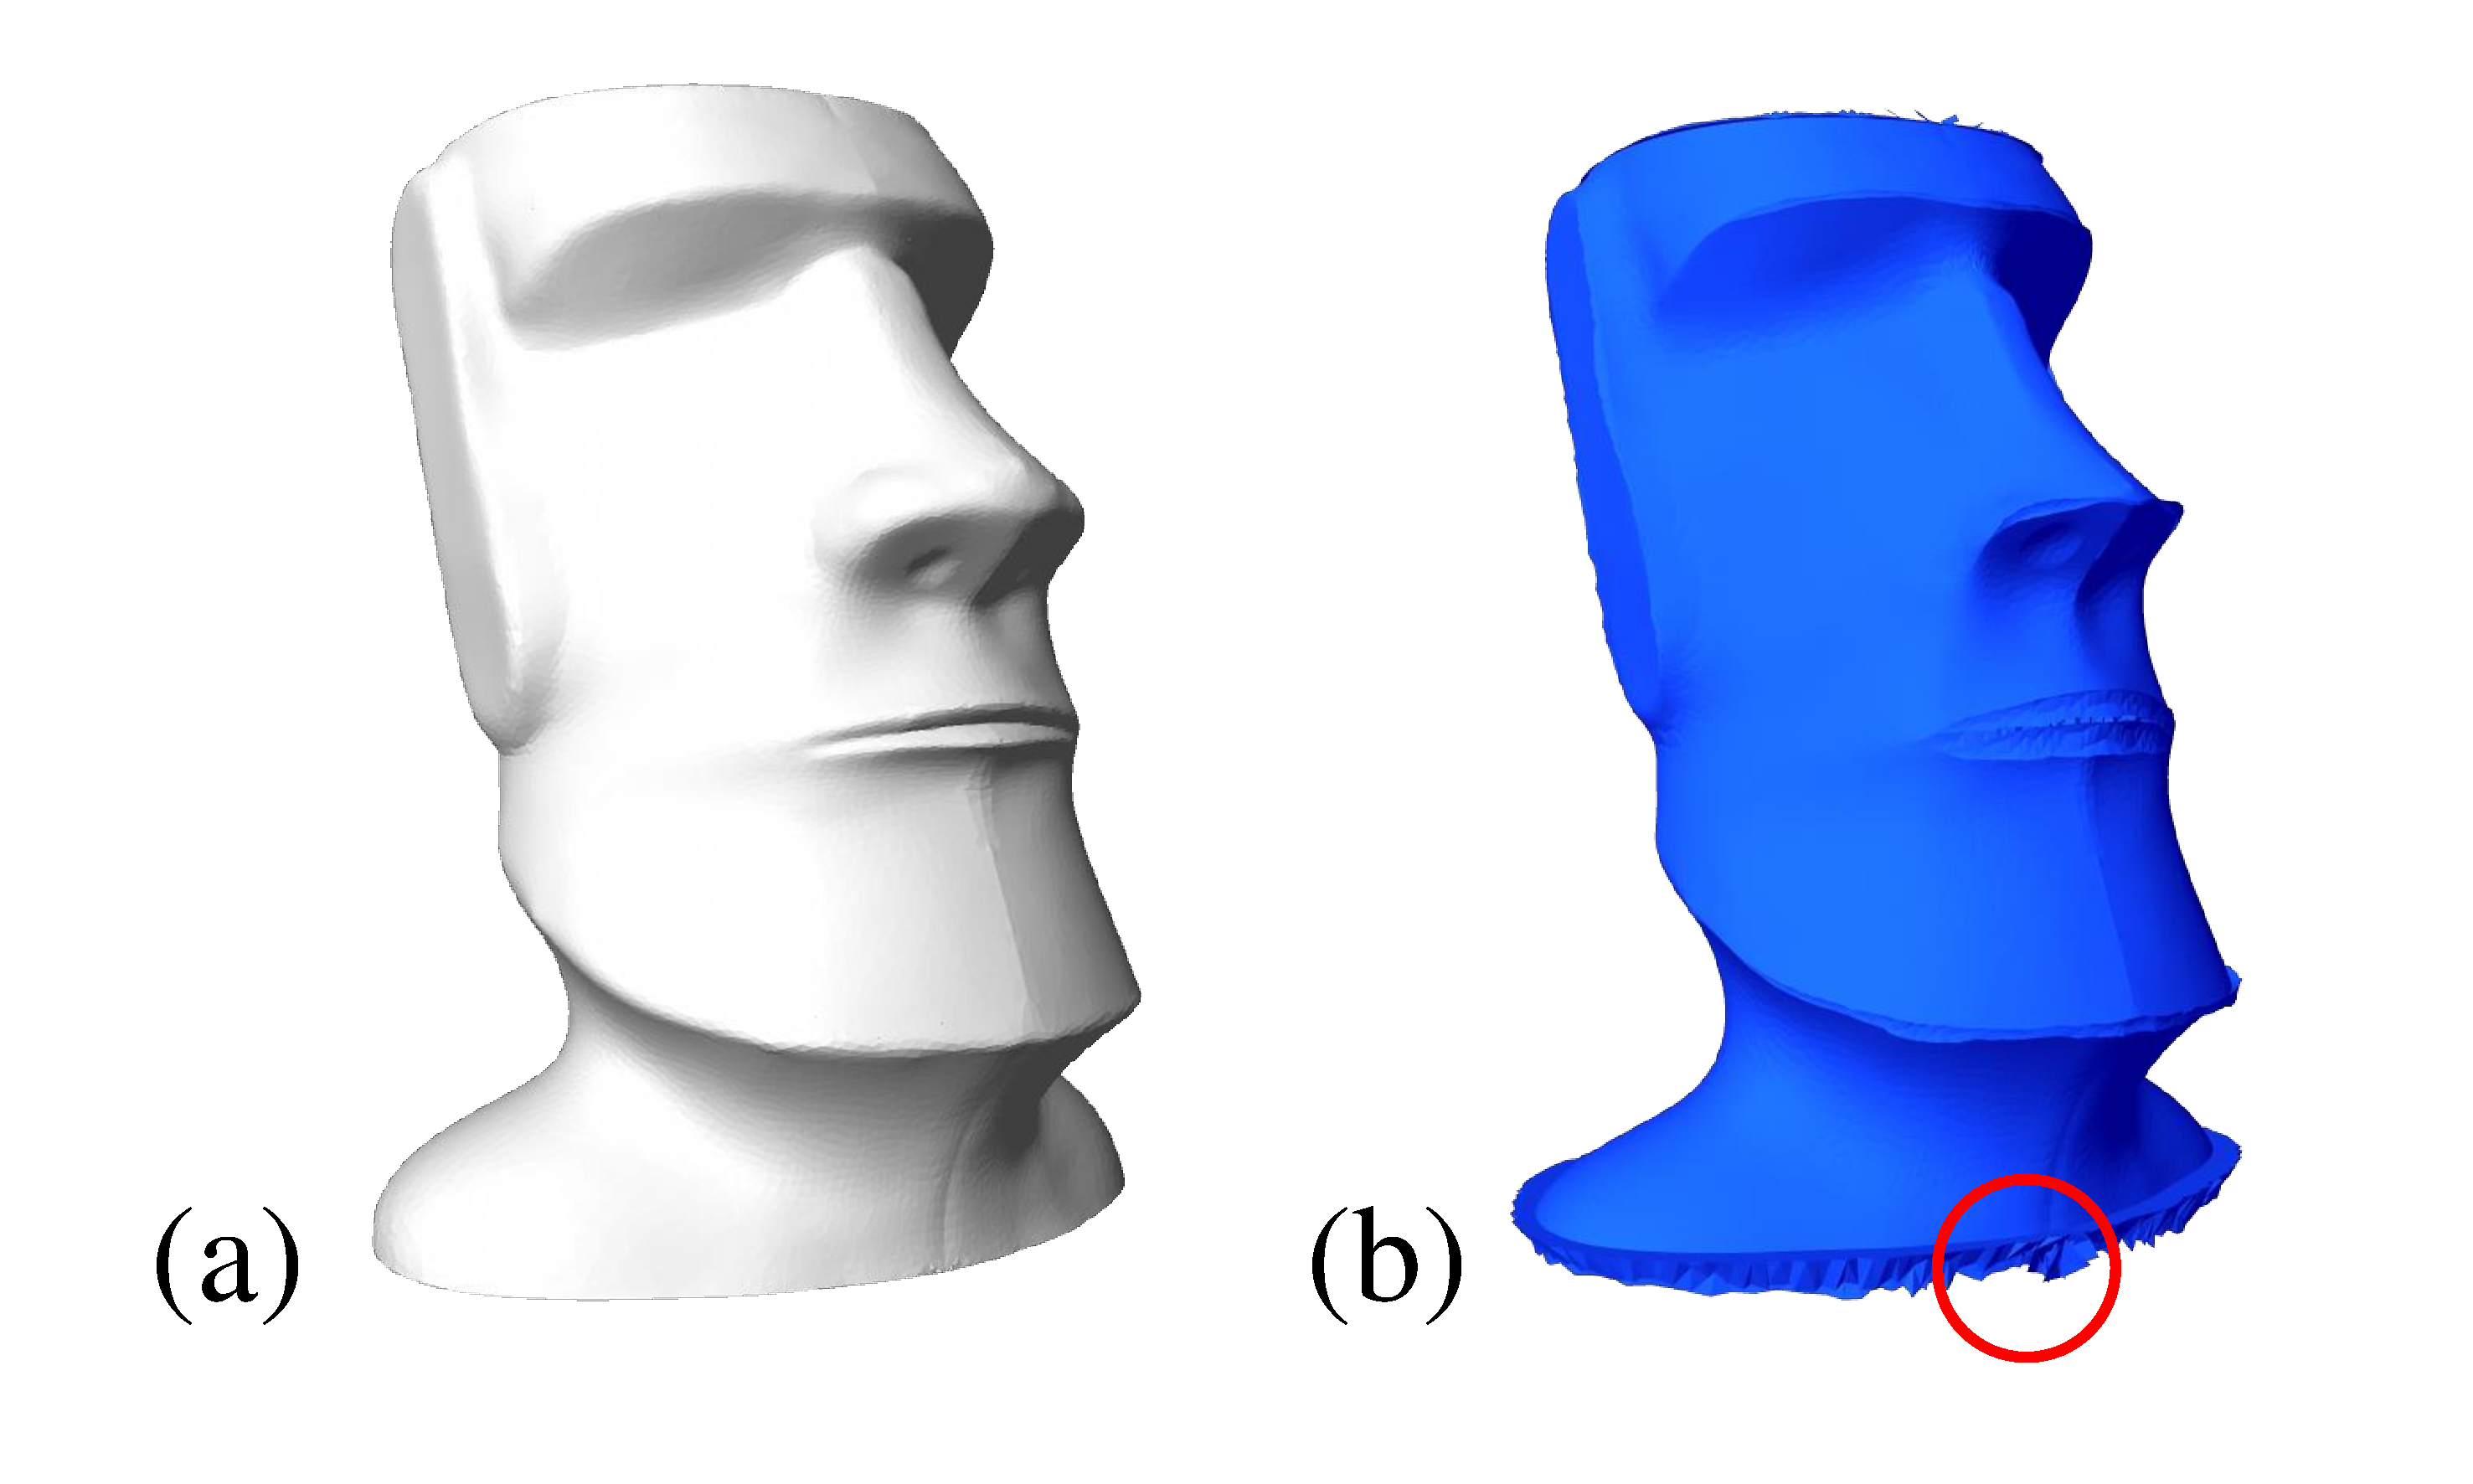
\includegraphics[width=1.0\linewidth]{figs/Shrink_mesh.pdf} 
% \caption{
% \ichao{Think about if we still need this figure.}
% (a) Original mesh (b) Shrunken mesh. Shrink the mesh along the vertex normals is the simple method, but sometimes the mesh will be broken.}
% \label{fig:shrink_mesh}
% \end{figure}
To prevent this problem, we instead voxelize the original object, and remove the voxels that cover the original surface.
\chireplace{And}{Moreover,} we use the \chireplace{outer surface}{outermost surface} of the remaining voxels as our inner surface for \chinky{solid mesh} (\figname~\ref{fig:inner_surface}).
% use the voxelized mesh to handle it. 
% First, we voxelize the original mesh. 
% Then, we choose the outer surface of the voxelized result and combine the original mesh to get the new mesh which has outer and inner surface. 
% The inner surface generation process is illustrated in \figname~\ref{fig:inner_surface}.

\begin{figure}[ht]
\centering
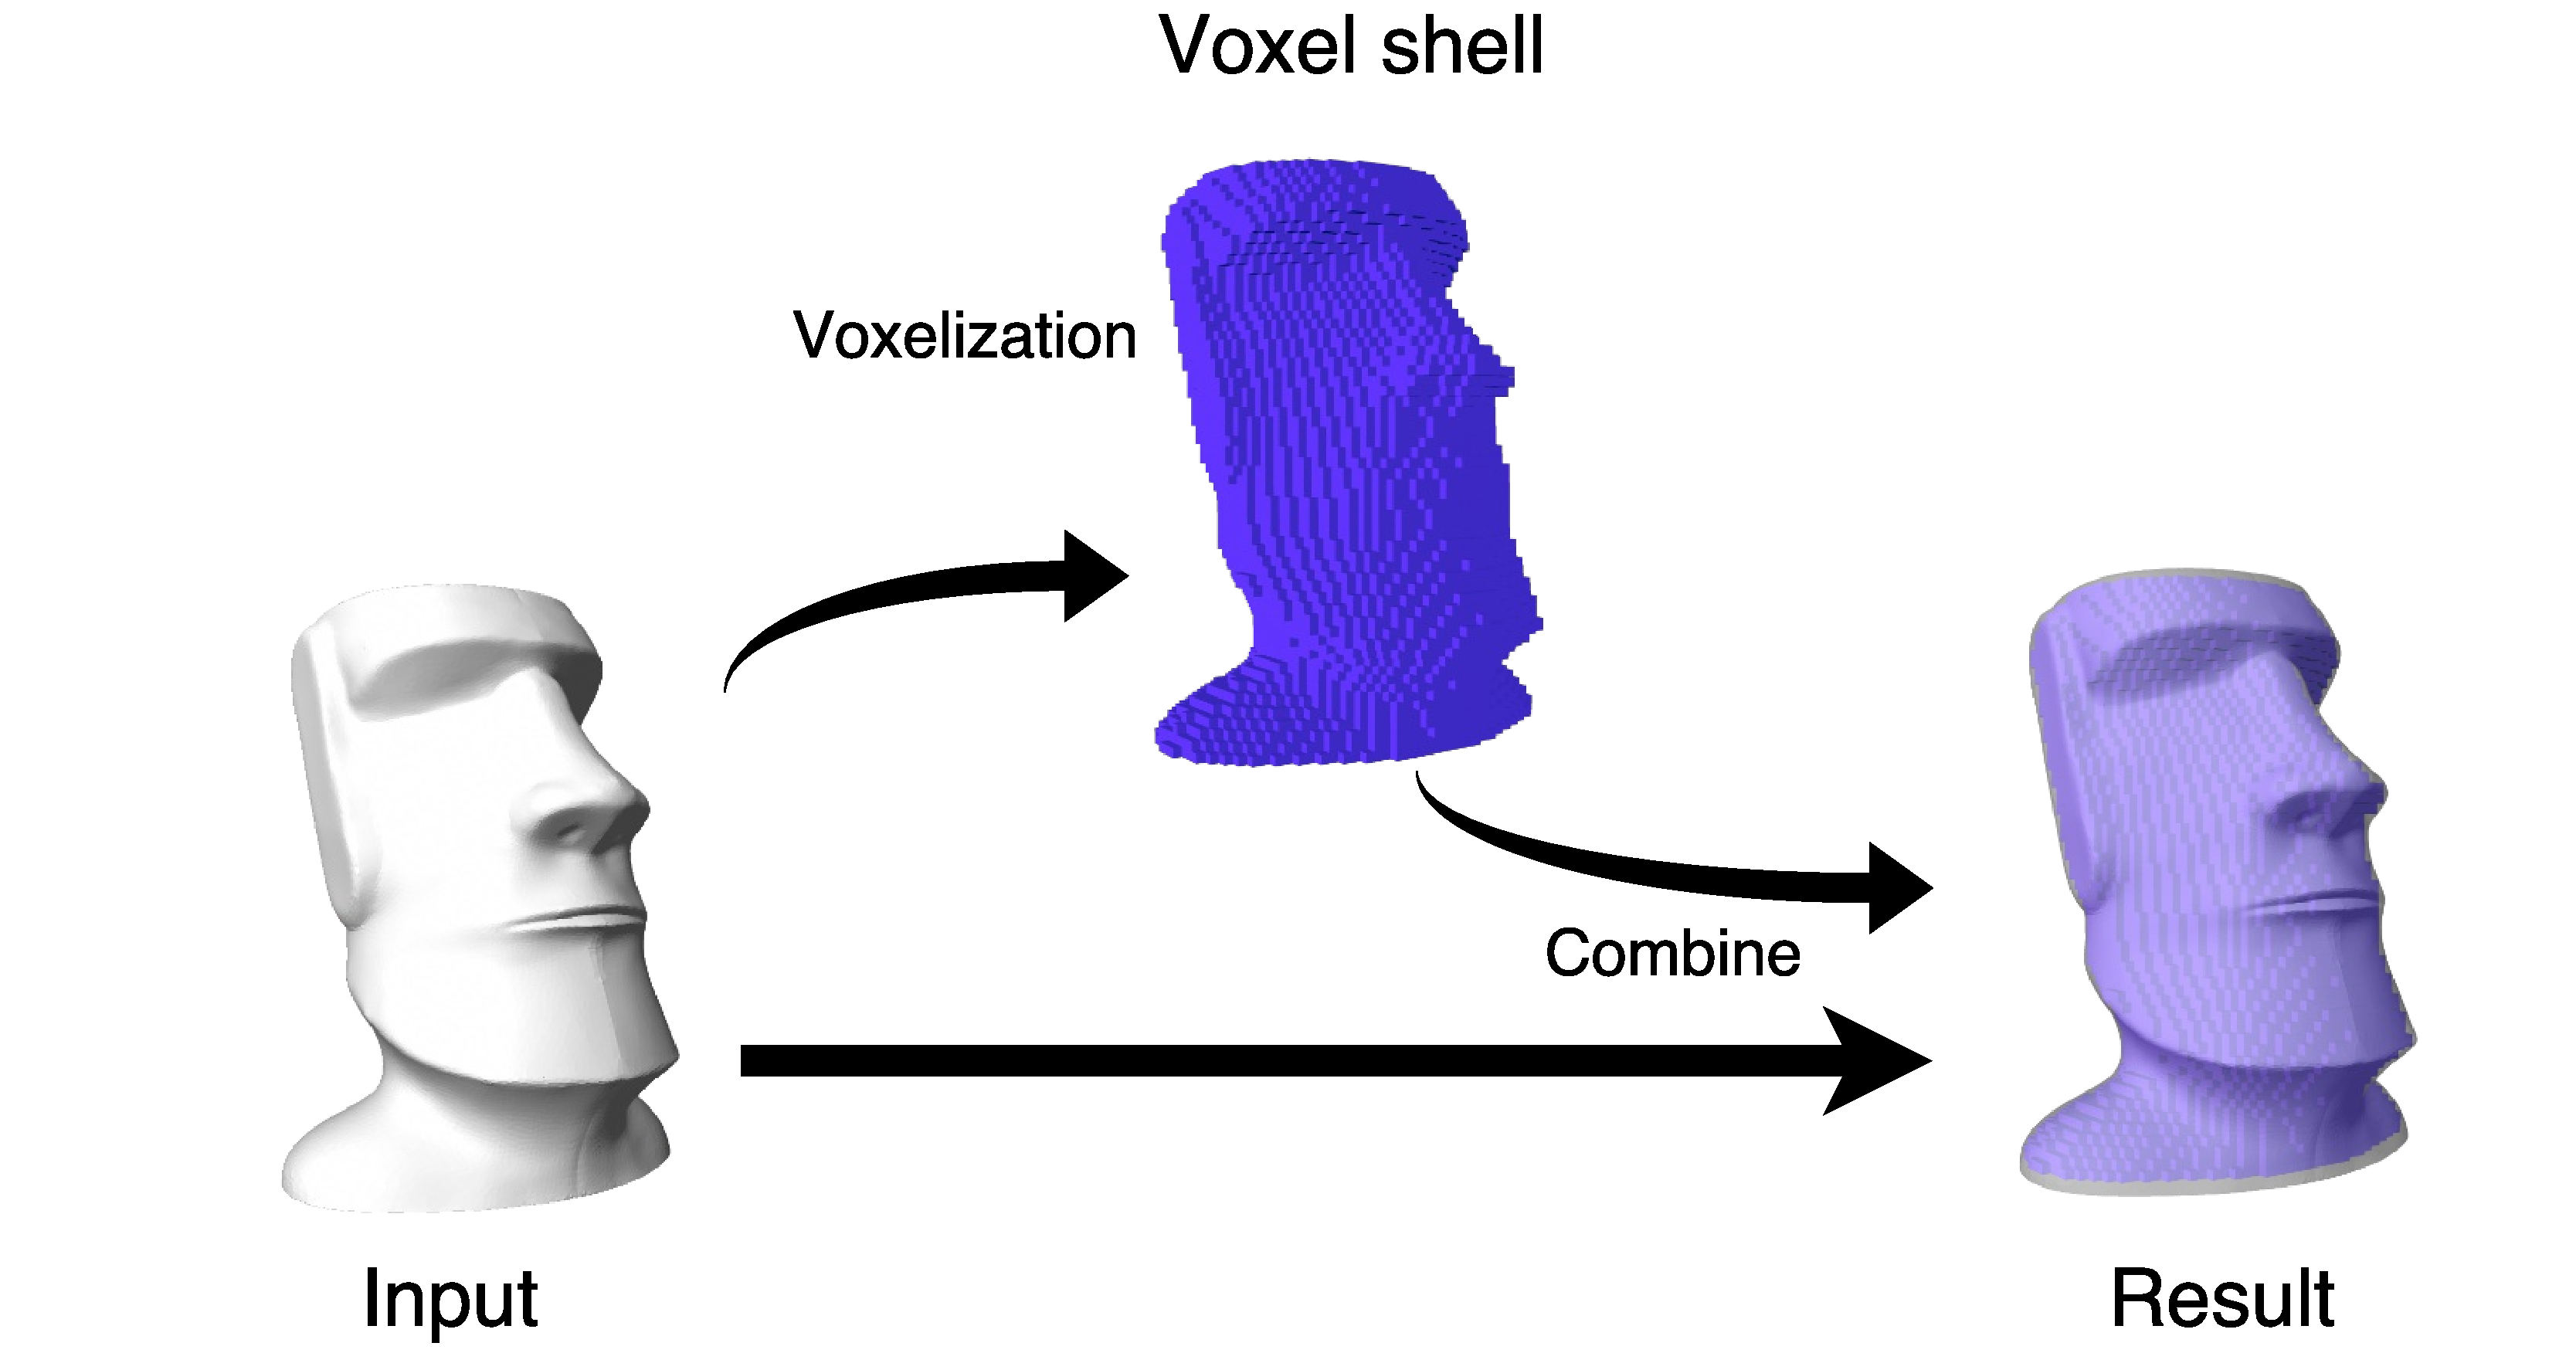
\includegraphics[width=1.0\linewidth]{figs/inner2.pdf} 
\caption{Inner surface generation method.}
\label{fig:inner_surface}
\end{figure}

% \subsection{Split mesh}
% In order to let user assemble the pieces easily, we use planar-cut method for mesh segmentation and find out the cut-plane in previous chapter. (see \secname ~\ref{sec:surf_part}) Then, we reference the function in open source software Blender~\cite{BLD} and modify it to be able to handle multiple plane cut. The alternative method help us get the segments, but the segments still can't be printed because of the hole between the outer and inner surface. We check each plane and find the vertices which align the plane. The vertex cluster can create a face which can fill the hole. But 3{D} printer just can print the mesh constructed by triangle. So, the new faces need to triangulate then the segment finally can be printed by the 3{D} printer. The details of split mesh process are in \figname~\ref{fig:split}.

% \begin{figure}[ht]
% \centering
% 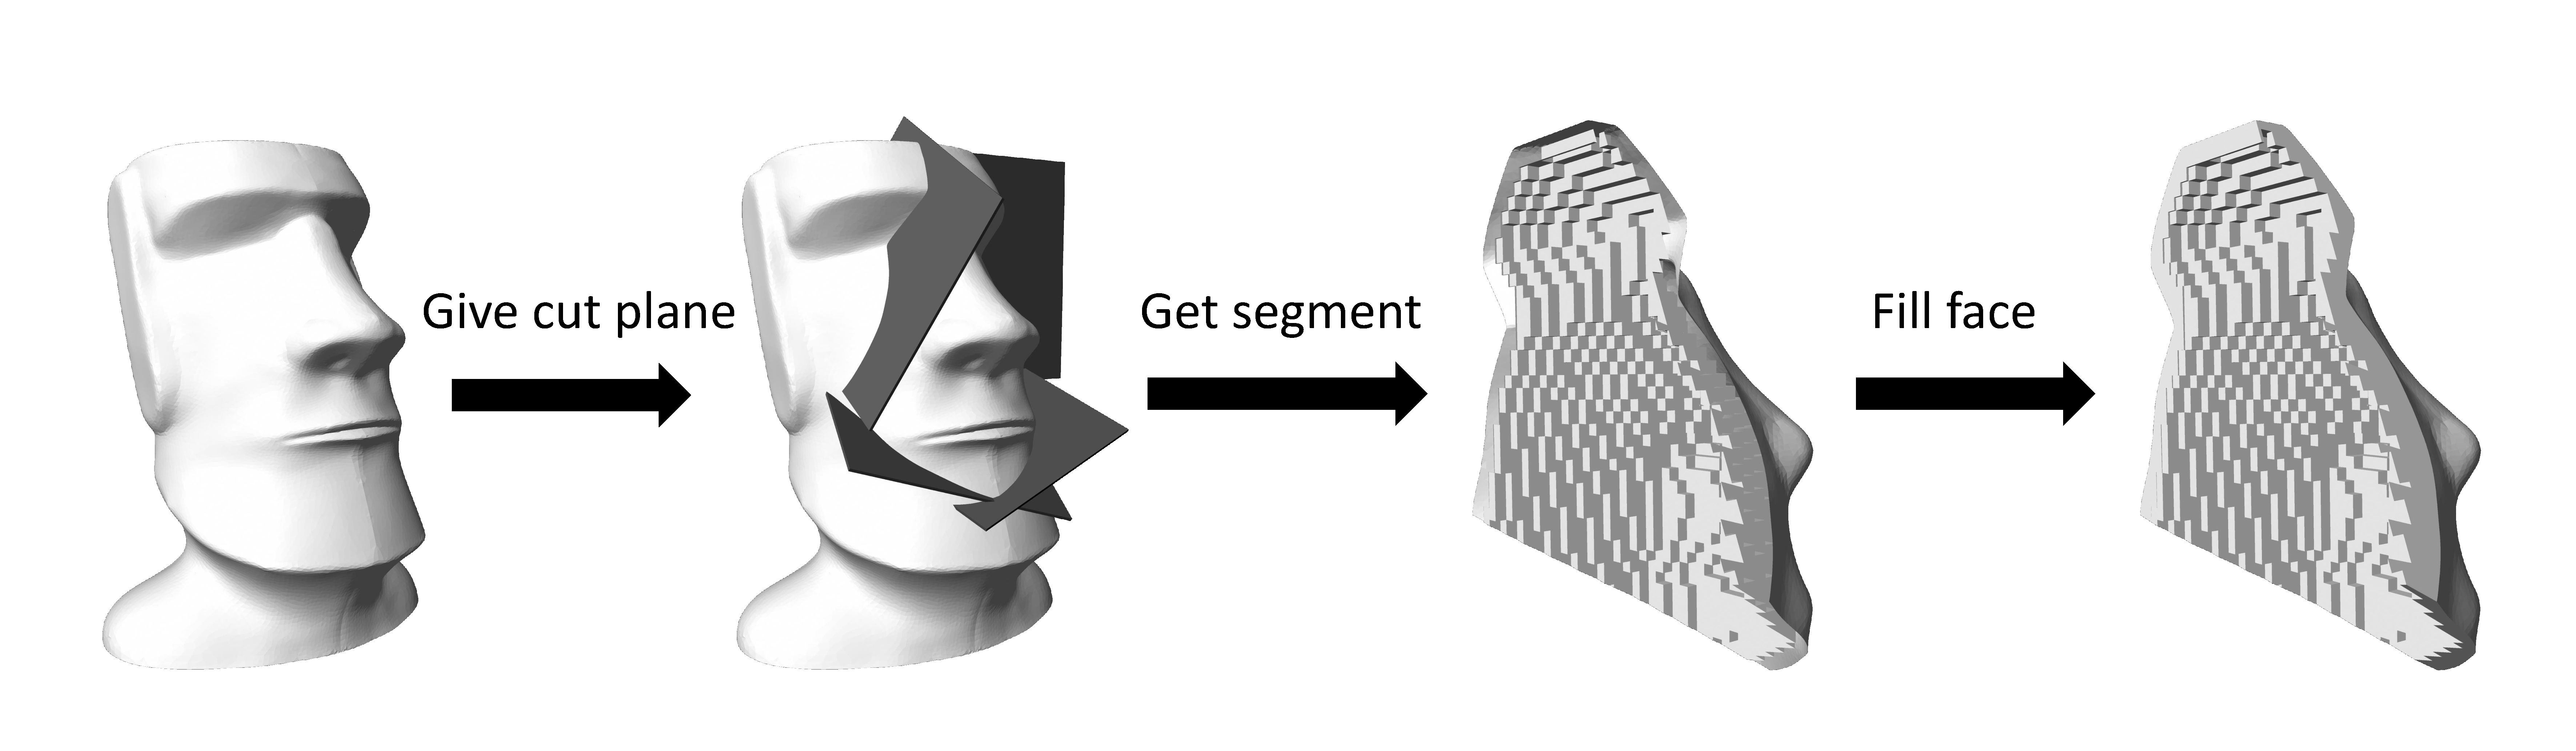
\includegraphics[width=1.0\linewidth]{figs/split.pdf} 
% \caption{Split mesh process.}
% \label{fig:split}
% \end{figure}
    
\subsection{Generate connector}
%After get the inner surface, we are able to use the partitioned results from graph cut to cut the surface into pieces. 
With the inner surface, we need to place connectors on it to connect between inner Zometool structure and outer shells.
% After get the split pieces, we need to connect the inner Zometool surface with these cutting pieces.
% But the pieces have to generate some connection to connect the inner Zometool structure. 
Two potential designs for building these connectors are:
\begin{enumerate}
\item Dig holes on the surface and use the Zometool rods to connect both inner and outer structure (\figname~\ref{fig:exp_connector} (a)).
\item  Grow Zometool tenons on the \chinky{inner} surface instead (\figname~\ref{fig:exp_connector} (b)).
\end{enumerate}
We will elaborate how we implement both designs and discuss the pros and cons of both designs in the following paragraph.
% The following context will discuss more detail.
% For example, the connection can dig some holes on the surface and use the Zometool rod to connect the structure.(in Fig 4 (a)). 
% The other method is grow Zometool tenons on the surface.(in Fig 4 (b)) 
\subsubsection{Dig holes}
As observed, naively digging holes on the inner surface is likely to break the outer surface.
Instead, we have to grow additional structure that replicate\chinky{s} Zome-ball, which is called ``virtual ball'' on the inner surface.
And we dig holes on this virtual ball to connect with \chinky{the} Zometool structure using \chireplace{z}{Z}ometool struts.
However, as the objects usually printed with support materials generated by 3D printer\chinky{s}, we observed that these support materials \chireplace{will greatly}{would hugely} reduce the quality of these holes.
The major reason is that the holes are filled with the support materials and it is \chireplace{really hard}{quite difficult} to \chireplace{clean}{remove} all of them.
As a result, the Zometool struts cannot be inserted well (\figname~\ref{fig:exp_connector} (a)).
To address this issue, practically we can change the printing directions, e.g.\chinky{,} place the holes face upward to the printing plate so that no support materials will be printed inside the holes.
However, this means that the outer surface is attached to the support materials, and the final printed appearance will be pretty poor.
The issue cannot be handled well given the limited precision of consumer-level 3D printer.
Hence, we propose an alternative connector design.
% If we want to dig some connecting holes on surface, we can't directly dig it because it might break the outer surface.
% To deal with it, the inner surface have to grow additional materials for digging. 
% We put a new Zome-ball called "virtual ball" on the inner surface which can have the additional materials for digging holes. 
% Then we can dig the holes on the virtual ball, thus the outer shell will not be broken. 
% The rods can use holes for connecting the main structure. 
% The downside of this approach is that shapes are usually printed with support materials, and the dug hole are usually filled with these materials. 
% If the support don't clean very well, the Zometool rods can't insert it. (see \figname~\ref{fig:exp_surface_dig}(b)) 
% In order to prevent the support material from generating in the holes during printing, we have to place the holes face upward to the printing plate. 
% The part which attaches the support materials always have worse quality. The holes face upward to the printing plate means that the outer surface is attached by the support materials, the final assembled result quality will be very poor.
% However, 3{D} printing can't print without the support material, the dig hole will fill with support material. 
% Due to the low precision issues for most of the consumer 3D printers, it is impractical to generate clean holes for Zometool tenon to plug in.
% Hence, we design an alternative approch to generate the connectors.
% If we don't clean the support clearly, the Zometool rod can't insert it. Beside, Zometool tenon is very small, the holes we dig are also small. The support material is very difficult to clean clearly. So we give up this method.
    
\subsubsection{Grow tenons on surface}
Zometool's tenon is a very small object, it fit perfectly on the Zome-ball and make\chinky{s} the structure pretty robust. 
However, the size of tenon is a strong challenge for the 3{D} printer due to it's limited precision. 
Beside, same object\chinky{s} will be printed differently under different orientations because the way of support printing.
In order to verify our 3{D} printer (Ultimaker 3 \footnote{https://ultimaker.com/en/products/ultimaker-3}) is able to print the tenons, we design an exhaustive experiment as follow:
we use Ultimaker 3 to print three different tenon of Zometool (rectangle, pentagon, triangle), each print in twenty-seven directions. 
As a result, we found out that even under the lowest precision (``fast print'' mode in Ultimaker 3), the printed tenons can still perfectly fit into the slots on the Zometool balls.
Compared to dig holes on \chinky{the inner} surface, it is also easier to \chireplace{clean}{remove} the printed support materials on the printed tenons.
Given it's easier \chireplace{clean up}{cleanup} and more robust structure, we use this design to connect the inner Zometool structure and outer shells (see \figname~\ref{fig:exp_connector} (b)). 

And we decide how many tenons on each outer shell with \chinky{the } following process:
We shoot rays from each slot on a single Zome-balls in the optimized Zometool structure $\mathbf{S}$, and record whether it intersect\chinky{s} with the surface.
We repeat this examination on all of the 62 slots on the Zome-balls, and we grow tenons on the surface along the direction with the most ray-surface intersections.
% Finally, we grow tenons on surface 
% We search the nearest node on inner Zometool structure on split piece by graph cut for each triangle. 
% There are sixty-two slots on the Zome-ball, it means we can get sixty-two directions to grow the tenons. 
% We choose the direction which can grow most tenons on the surface to make a strong connection on the inner Zometool structure.

% \subsubsection{Discussion}
% \textbf{Dig holes} and \textbf{Grow tenons on surface} are two different methods for generating connection to the main inner structure. Each of method has disadvantages. \textbf{Dig holes} has problems of cleaning support material and quality. \textbf{Grow tenons on surface} has a problem that sometimes the tenons are broken when user clean up the printing support. The reason is the connection place will get the weak structure during slicer for 3D printing if we just insert the tenons mesh on surface directly. In order to reinforce the structure, we use CSG operation to combine the surface and tenons structure. Then the combine results are very robust. Our method want to approach \textbf{generating easily} and \textbf{good quality}. The problem of \textbf{Dig holes} are opposite to our main goal. So, we choose \textbf{Grow tenons on surface} for our generating connection to the main inner structure. 
    
\begin{figure}[ht]
\centering
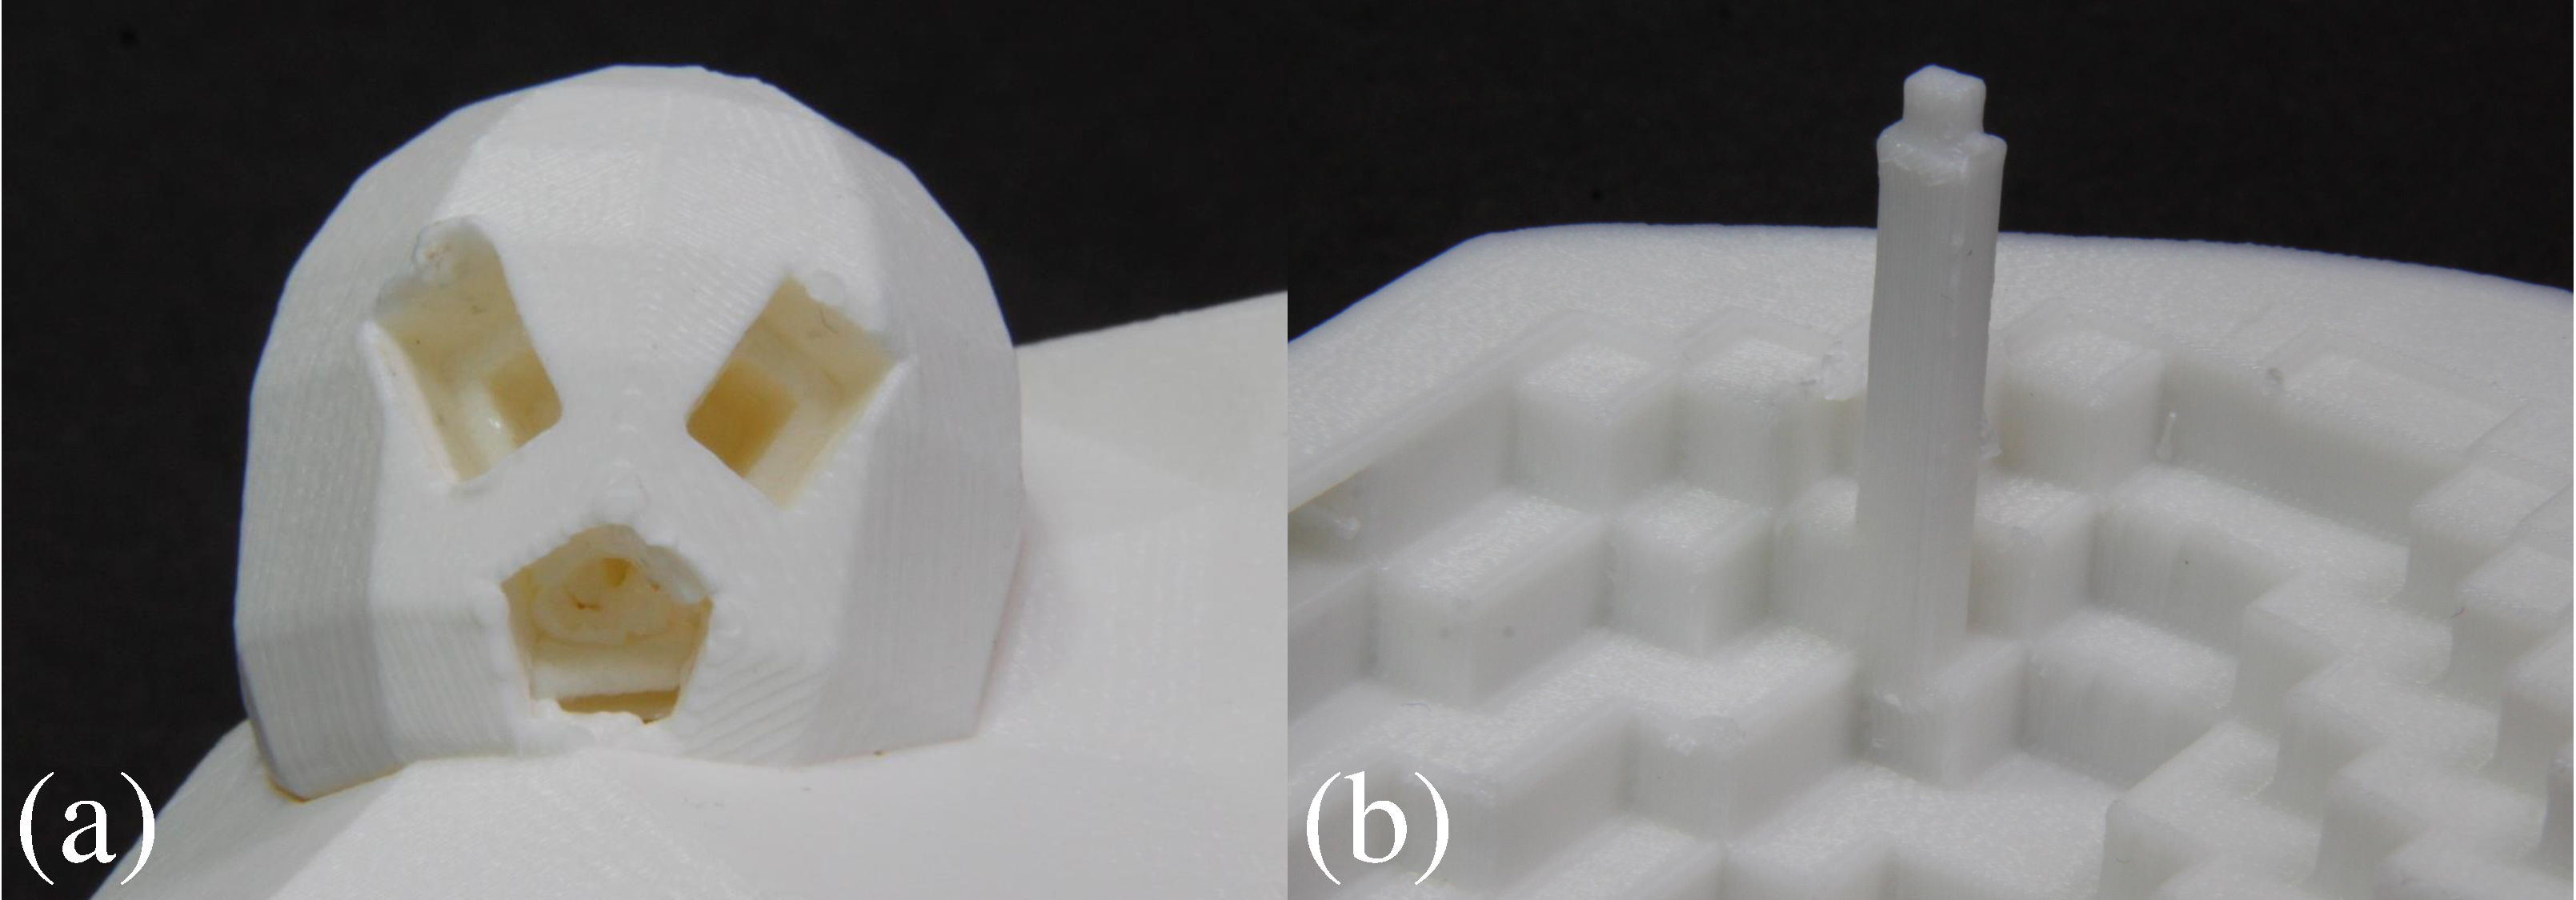
\includegraphics[width=1.0\linewidth]{figs/surface_connection.pdf} 
\caption{
Connector design : Dig holes on inner surface (a) and grow tenons on surface (b).
We can see that the materials in the digged hole can not be cleaned well in (a), so the Zometool struts can not be inserted well.
}
\label{fig:exp_connector}
\end{figure}

% \begin{figure}[ht]
% \centering
% 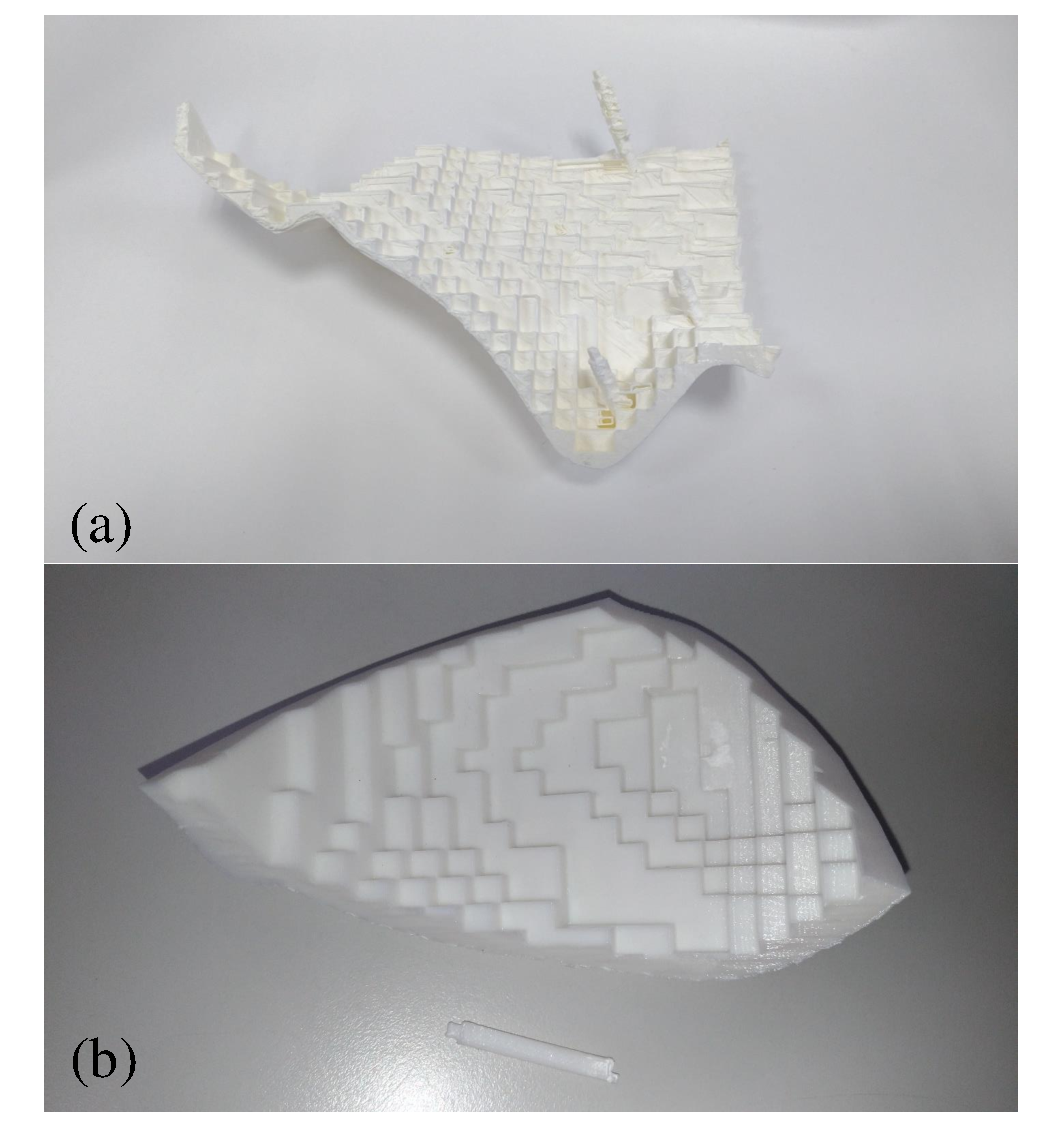
\includegraphics[width=1.0\linewidth]{figs/grow_tenon.pdf} 
% \caption{Experiment: Grow tenons on surface (a) result (b) tenons broken}
% \label{fig:exp_surface_tenon}
% \end{figure}

\section{Result}
\label{sec:result}

\subsection{Experiment environment}
We implement ZomeFab in C++ (most) and Python on desktop PC with 3.4GHz CPU and 16GB memory. 
The assembling processes are showed in Table \ref{tab:result_ZomeFab_real}. The inner structure is built by Zometool which can construct a strong structure easily. 
The outer surfaces are printed by Ultimaker 3, a low-cost FDM 3{D} printer with 0.2m x 0.2m x 0.2m printing volume and PLA material. The time it takes to assemble the fabricated parts for these mesh ranges from few minutes to around an hour, depending on the number of parts.

\subsection{Evaluation}
We evaluate the material cost and fabrication time between Zomefab and solid mesh with simple partition. We use CURA (version 2.7.0), a slicer software for 3{D} printing, to help us evaluate it. The software will evaluate the fabrication time and the a amount of materials if the volume of input mesh is printable. In Table \ref{tab:result_material} and Table \ref{tab:result_time}, we demonstrate four experiments for each mesh, print hollowed with 20\% infill and print solid by Zomefab and baseline that partitions a solid object into 3D printable parts. \\
The experiment assumes two conditions: 
\begin{enumerate}
\item Baseline is that it prints input mesh as pieces and use 3D printer only. (We use octree for segmentation)
\item In multiple 3{D} printer experiment, we have enough  3D printers like the maker’s studio that we can print all pieces simultaneously. 
\end{enumerate}
The following context will discuss the material cost and the printing time.

\subsubsection{Material cost}
Material cost sets printing material: 0.56 USD/meter (Ultimaker official PLA material from official online shop, 90 meters sell 50 USD), Zometool rod: 0.19 USD/rod (from Zometool official online shop, 100 rods sell 19 USD) and Zome-ball: 0.29 USD/ball (from Zometool official online shop, 100 Zome-balls sell 29 USD) for our experiments. In Table \ref{tab:result_material}, all of experiments show that our method cost less material than baseline. Even if we print the result in 20\% fill rate, we also saved about 25\% of the material cost.

\subsubsection{Printing time}
In Table \ref{tab:result_time}, we demonstrate the statistical comparison of printing time between single 3{D} printer and multiple 3{D} printers. In single 3{D} printer, the fabrication time is more than baseline in 20\% infill rate. We propose that our mesh's complexity is higher than baseline testing mesh. In multiple 3{D} printers, we assume that we have enough 3{D} printers, so our method just has to wait the piece which has the most printing time. The statistics show that our method printing time is absolutely faster than baseline in different fill rate by multiple 3{D} printers. It demonstrates that our method's printing time will decrease if user can use more 3{D} printers. (See \figname~\ref{fig:multi_printer}) If the user just has single 3{D} printer and wants to get a exquisite result, our method can also get lower cost and fabrication time.

\subsection{Zometool Use}
Table \ref{tab:result_Zometool} shows the quantity of Zometool rods and balls about each result. In \secname~\ref{sec:Zometool}, we use smallest blue rods to make the zome-cube for the simple repeated structure in order to make the best-fit initial structure. The bigger structure will use more smallest blue rods (${b_0}$). Also, Zometool is created by unique math model, it has some special conditions: 
\begin{enumerate}
\item The blue rods and yellow rods are more compatible than the blue rods and red rods. 
\item  The longest rod only can be replaced by one shortest and middle rod in same color.
\end{enumerate}

So the number of smallest
yellow rods will increase if we use more smallest blue rods. Except the smallest yellow and blue rods, the other rods are used few or none in our simulated annealing rule.

%The red rods, middle rods and long rods in all colors used few or none in our simulated annealing rule.

\begin{table*}[ht]
\centering
\resizebox{1.\linewidth}{!} {
\begin{tabular}{|c|c|c|c c c|c|} \hline
 \multirow{2}*{Mesh} & \multirow{2}*{Infill Method} & \multirow{2}*{Fabrication Method} & \multicolumn{3}{c|}{Material Cost (USD)} & Efficiency (Saved)\\\cline{4-7} 
 & & & 3D printing & Zometool & Overall (sum) & Material \\ \hline
 
 \multirow{4}*{Moai} & \multirow{2}*{Hollow} & Zomefab & 82.56 & 70.57 & 153.13  & \multirow{2}*{58.36\%} \\ 
 &  & Baseline & 367.78 &  & 367.78 &\\\cline{2-7}
 & \multirow{2}*{Solid} & Zomefab & 170.9 & 70.57 & 241.47  & \multirow{2}*{82.60\%} \\
 &  & Baseline & 1387.92 & & 1387.92 &\\ \hline
  
 \multirow{4}*{Squirrel} & \multirow{2}*{Hollow} & Zomefab & 100.38 & 77.55 & 177.93 & \multirow{2}*{64.67\%} \\ 
 &  & Baseline & 503.56 & & 503.56  &\\\cline{2-7}
 & \multirow{2}*{Solid} & Zomefab & 213.96 & 77.55 & 291.51  & \multirow{2}*{85.42\%}\\
 &  & Baseline & 2000.00 & & 2000.00 &\\ \hline
 
 \multirow{4}*{Doraemon} & \multirow{2}*{Hollow} & Zomefab & 101.38 & 76.34 & 177.72 & \multirow{2}*{24.43\%}\\ 
 &  & Baseline & 235.16 & & 235.16 &\\\cline{2-7}
 & \multirow{2}*{Solid} & Zomefab & 227.78 & 76.34 & 304.12 &  \multirow{2}*{68.24\%}\\
 &  & Baseline & 957.42 & & 957.42 &\\ \hline
 
\multirow{4}*{Totoro} & \multirow{2}*{Hollow} & Zomefab & 72.32 & 61.48 & 133.80 & \multirow{2}*{27.84\%}\\ 
 &  & Baseline & 185.41 & & 185.41 &\\\cline{2-7}
 & \multirow{2}*{Solid} & Zomefab & 148.26 & 61.48 & 209.74 &  \multirow{2}*{71.17\%} \\
 &  & Baseline & 727.51 & & 727.51 &\\ \hline
 
\multirow{4}*{Iron Man} & \multirow{2}*{Hollow} & Zomefab & 73.99 & 57.76 & 131.75 & \multirow{2}*{32.45\%} \\ 
 &  & Baseline & 195.04 & & 195.04 &\\\cline{2-7}
 & \multirow{2}*{Solid} & Zomefab & 149.67 & 57.76 & 207.43 &  \multirow{2}*{76.50\%} \\
 &  & Baseline & 829.88 & & 829.88 &\\ \hline
 
\end{tabular}
}
\caption{ZomeFab's performance on saving material as compared to a baseline method.}
\label{tab:result_material}
\end{table*}

\begin{table*}[ht]
\centering
\resizebox{1.\linewidth}{!} {
\begin{tabular}{|c|c|c|c c c| c c c|c | c|} \hline
 \multirow{2}*{Mesh} & \multirow{2}*{Infill Method} & \multirow{2}*{Fabrication Method} & \multicolumn{3}{c|}{Single 3{D} Printer Fabrication Time (hours)} & \multicolumn{3}{c|}{Multiple 3{D} Printer Fabrication Time (hours)} & \multicolumn{2}{c|}{Efficiency (Saved)}\\\cline{4-11} 
 & & & 3D printing & Zometool & Overall (sum) & 3D printing & Zometool & Overall (max) & Single & Multiple\\ \hline
 
 \multirow{4}*{Moai} & \multirow{2}*{Hollow} & Zomefab & 293.97 & 2.5 & 296.47 & 72.58 & 2.5 & 75.08 & \multirow{2}*{-34.23\%} & \multirow{2}*{67.14\%}\\ 
 &  & Baseline & 220.86 &  & 220.86 & 220.86 &  & 220.86 & &\\\cline{2-11}
 & \multirow{2}*{Solid} & Zomefab & 523.20 & 2.5 & 525.70 & 108.13 & 2.5 & 110.63 & \multirow{2}*{58.87\%} & \multirow{2}*{91.34\%}\\
 &  & Baseline & 1278.00 & & 1278.00 & 1278.00 & & 1278.00 & &\\ \hline
  
 \multirow{4}*{Squirrel} & \multirow{2}*{Hollow} & Zomefab & 355.05 & 3.0 & 358.05 & 53.82 & 3.0 & 56.82 & \multirow{2}*{-32.78\%} & \multirow{2}*{78.93\%}\\ 
 &  & Baseline & 269.66 & & 269.66 & 269.66 & & 269.66 & &\\\cline{2-11}
 & \multirow{2}*{Solid} & Zomefab & 643.65 & 3.0 & 646.65 & 93.97 & 3.0 & 96.97 & \multirow{2}*{52.19\%} & \multirow{2}*{92.83\%}\\
 &  & Baseline & 1352.42 & & 1352.42 & 1352.42 & & 1352.42 & &\\ \hline
 
 \multirow{4}*{Doraemon} & \multirow{2}*{Hollow} & Zomefab & 356.60 & 4.0 & 360.60 & 53.83 & 4.0 & 57.83 & \multirow{2}*{-48.71\%} & \multirow{2}*{75.88\%}\\ 
 &  & Baseline & 239.8 & & 239.8 & 239.8 & & 239.8 & &\\\cline{2-11}
 & \multirow{2}*{Solid} & Zomefab & 643.65 & 4.0 & 647.65 & 93.97 & 4.0 & 97.97 & \multirow{2}*{67.48\%} & \multirow{2}*{95.08\%}\\
 &  & Baseline & 1991.7 & & 1991.7 & 1991.7 & & 1991.7 & &\\ \hline
 
\multirow{4}*{Totoro} & \multirow{2}*{Hollow} & Zomefab & 273.68 & 3.0 & 276.68 & 29.37 & 3.0 & 32.37 & \multirow{2}*{-46.26\%} & \multirow{2}*{82.89\%}\\ 
 &  & Baseline & 189.17 & & 189.17 & 189.17 & & 189.17 & &\\\cline{2-11}
 & \multirow{2}*{Solid} & Zomefab & 468.82 & 3.0 & 471.82 & 51.67 & 3.0 & 54.67 & \multirow{2}*{68.68\%} & \multirow{2}*{96.37\%}\\
 &  & Baseline & 1506.34 & & 1506.34 & 1506.34 & & 1506.34 & &\\ \hline
 
\multirow{4}*{Iron Man} & \multirow{2}*{Hollow} & Zomefab & 282.30 & 2.0 & 284.30 & 47.57 & 2.0 & 49.57 & \multirow{2}*{-39.37\%} & \multirow{2}*{75.53\%}\\ 
 &  & Baseline & 202.56 & & 202.56 & 202.56 & & 202.56 & &\\\cline{2-11}
 & \multirow{2}*{Solid} & Zomefab & 477.03 & 2.0 & 479.03 & 72.12 & 2.0 & 74.12 & \multirow{2}*{68.37\%} & \multirow{2}*{95.12\%}\\
 &  & Baseline & 1514.70 & & 1514.70 & 1514.70 & & 1514.70 & &\\ \hline
 
\end{tabular}
}
\caption{ZomeFab's performance on time as compared to a baseline method.}
\label{tab:result_time}
\end{table*}

\begin{figure*}[ht]
\centering
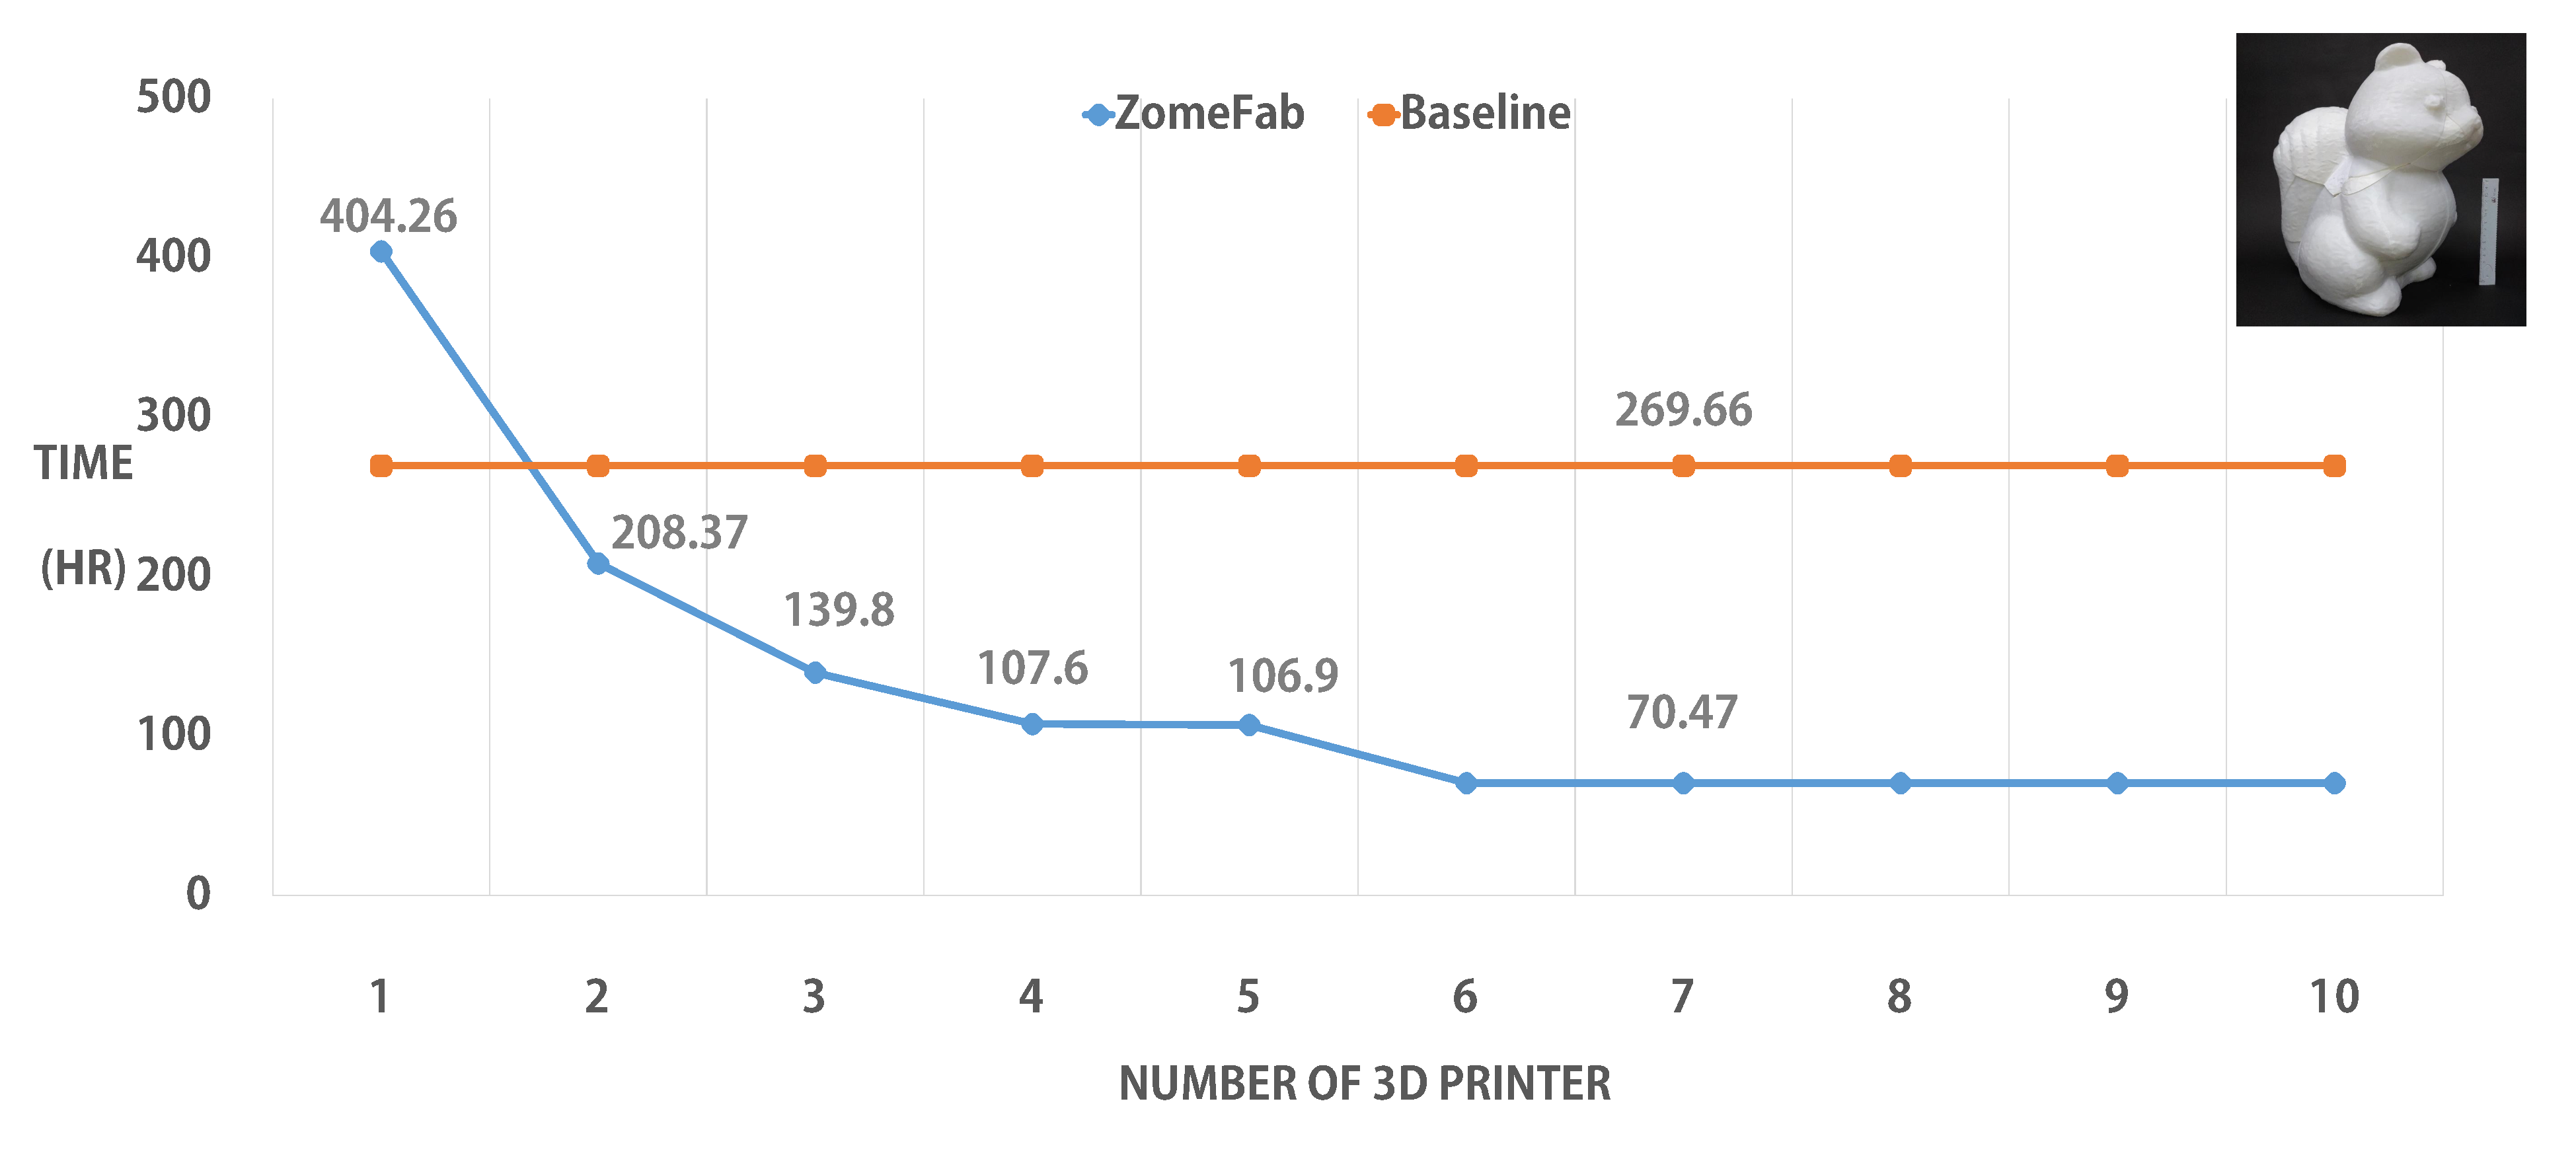
\includegraphics[width=1.0\linewidth]{figs/multi_printer.pdf} 
\caption{Printing time of Squirrel with different number of printers. If user use single 3D printer to print the result, our method's printing time will be more than baseline. The chart shows if the number of 3D printers are more than 2, the printing time will lower than baseline. If user has more than 6 3D printers, the printing time only has to wait the pieces which has the longest printing time.
}
\label{fig:multi_printer}
\end{figure*}

\begin{table*}[ht]
\centering
\resizebox{0.7\linewidth}{!} {
\begin{tabular}{|c|c|c|c|c|c|c|c|c|c|c|c|} \hline
\multirow{3}*{Mesh} & \multicolumn{10}{c|}{Zometool} & \multirow{3}*{Printing pieces}\\\cline{2-11} 
& \multicolumn{3}{c|}{Blue} & \multicolumn{3}{c|}{Red} & \multicolumn{3}{c|}{Yellow} & \multirow{2}*{Ball} & \\\cline{2-10} 
& S & M & L & S & M & L & S & M & L & & \\ \hline
Moai & 112 & 0 & 0 & 0 & 0 & 0 & 140 & 0 & 0 & 73 & 8 \\ \hline
Squirrel & 144 & 22 & 0 & 8 & 4 & 0 & 119 & 3 & 1 & 85 & 13 \\ \hline
Doraemon & 143 & 26 & 1 & 2 & 5 & 1 & 89 & 1 & 1 & 87 & 15 \\ \hline
Totoro & 95 & 0 & 0 & 0 & 0 & 0 & 137 & 0 & 0 & 60 & 18 \\ \hline
Iron Man & 93 & 0 & 0 & 0 & 0 & 0 & 124 & 0 & 0 & 57 & 10 \\ \hline
Owl & 115 & 0 & 0 & 0 & 0 & 0 & 159 & 0 & 0 & 70 & 15 \\ \hline
Pig & 61 & 12 & 0 & 10 & 8 & 0 & 53 & 6 & 0 & 47 & 10 \\ \hline
Slime & 132 & 0 & 0 & 0 & 0 & 0 & 182 & 0 & 0 & 80 & 14 \\ \hline
Lion & 78 & 0 & 0 & 0 & 0 & 0 & 101 & 0 & 0 & 50 & 8 \\ \hline
Bunny & 215 & 0 & 0 & 0 & 0 & 0 & 266 & 0 & 0 & 126 & 10 \\ \hline
\end{tabular}
}
\caption{Material usage for each result. Including Zometool and printing pieces.}
\label{tab:result_Zometool}
\end{table*}

% \begin{table*}[ht]
% \centering
% \resizebox{0.95\linewidth}{!} {
% \begin{tabular}{c} 
% 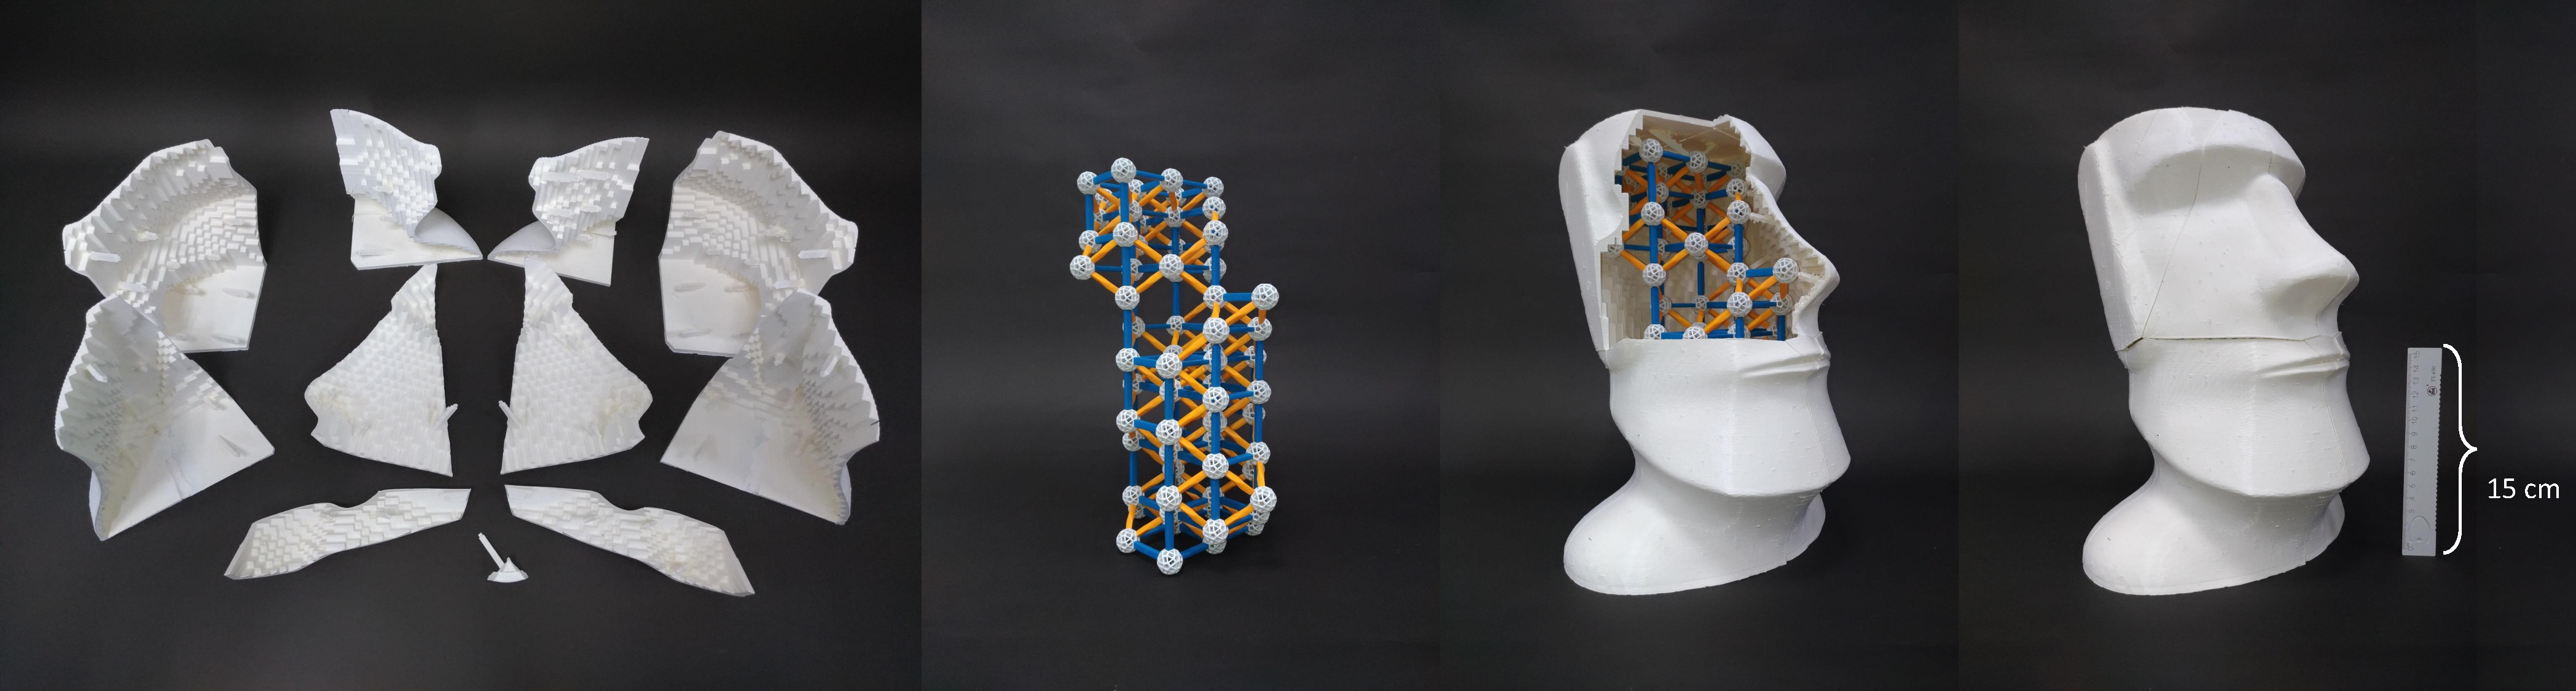
\includegraphics{figs/MOAI_real2.pdf} \\
% 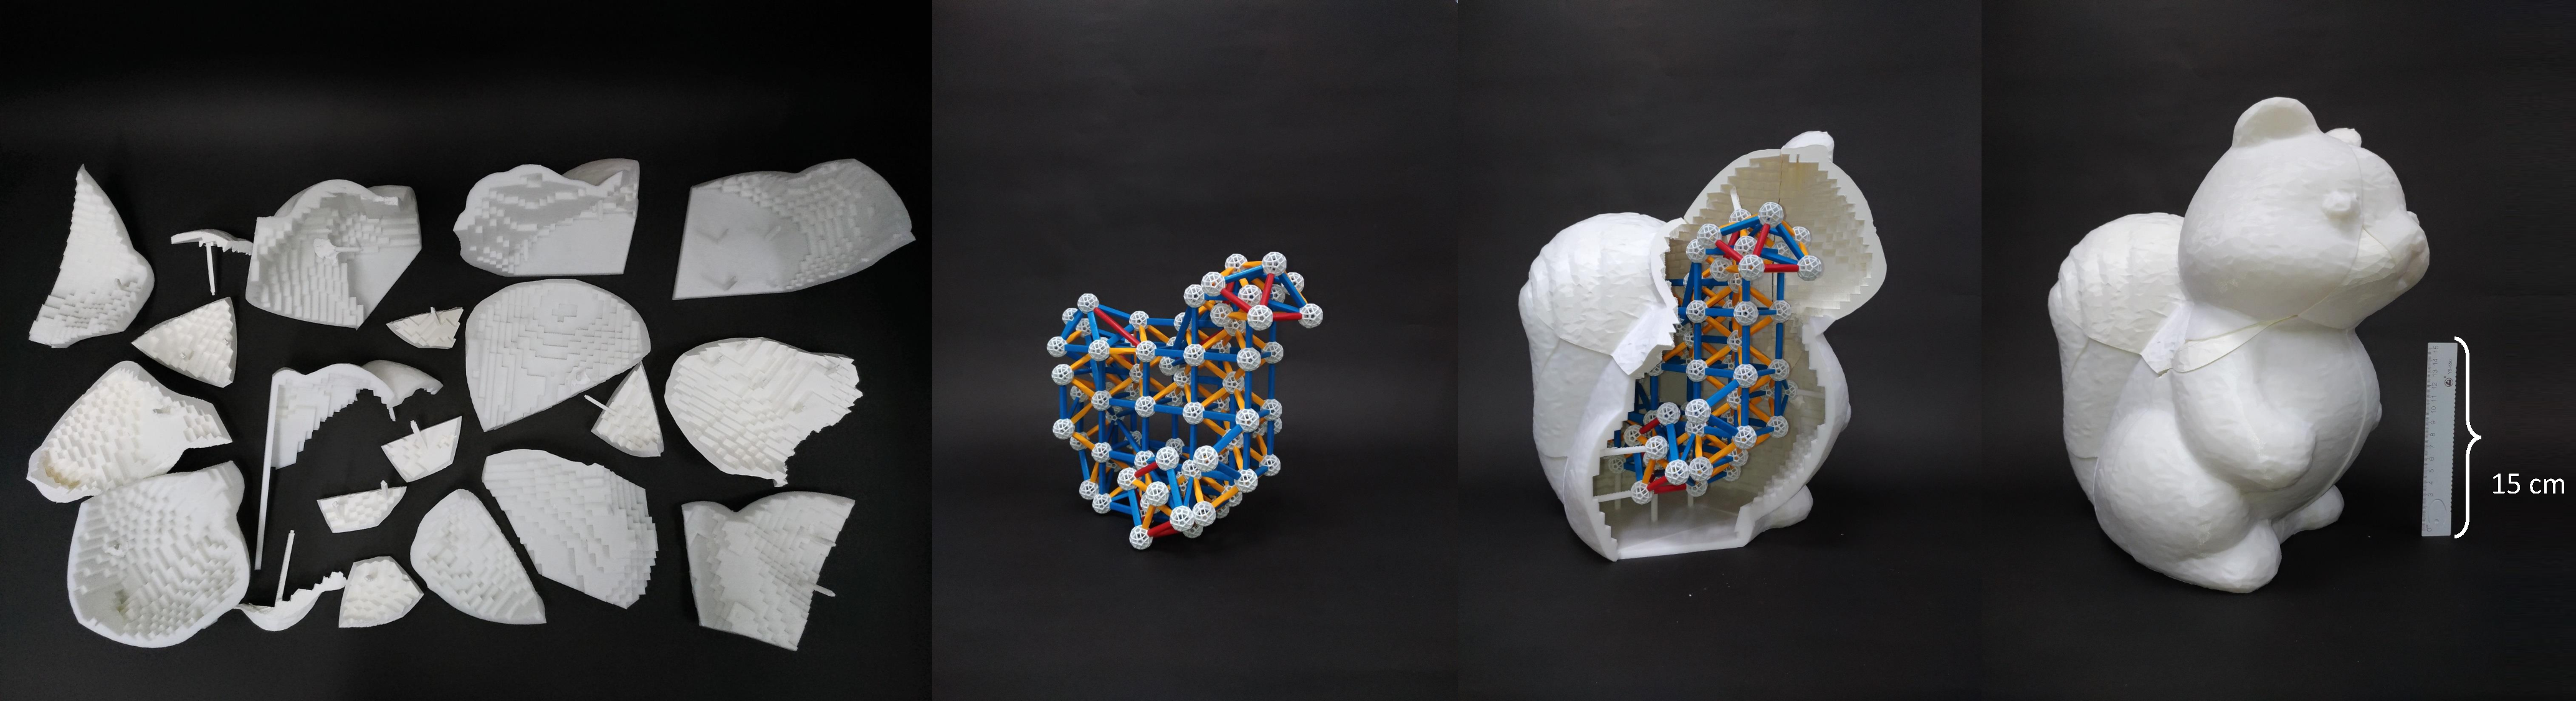
\includegraphics{figs/Squirrel_real2.pdf}\\
% 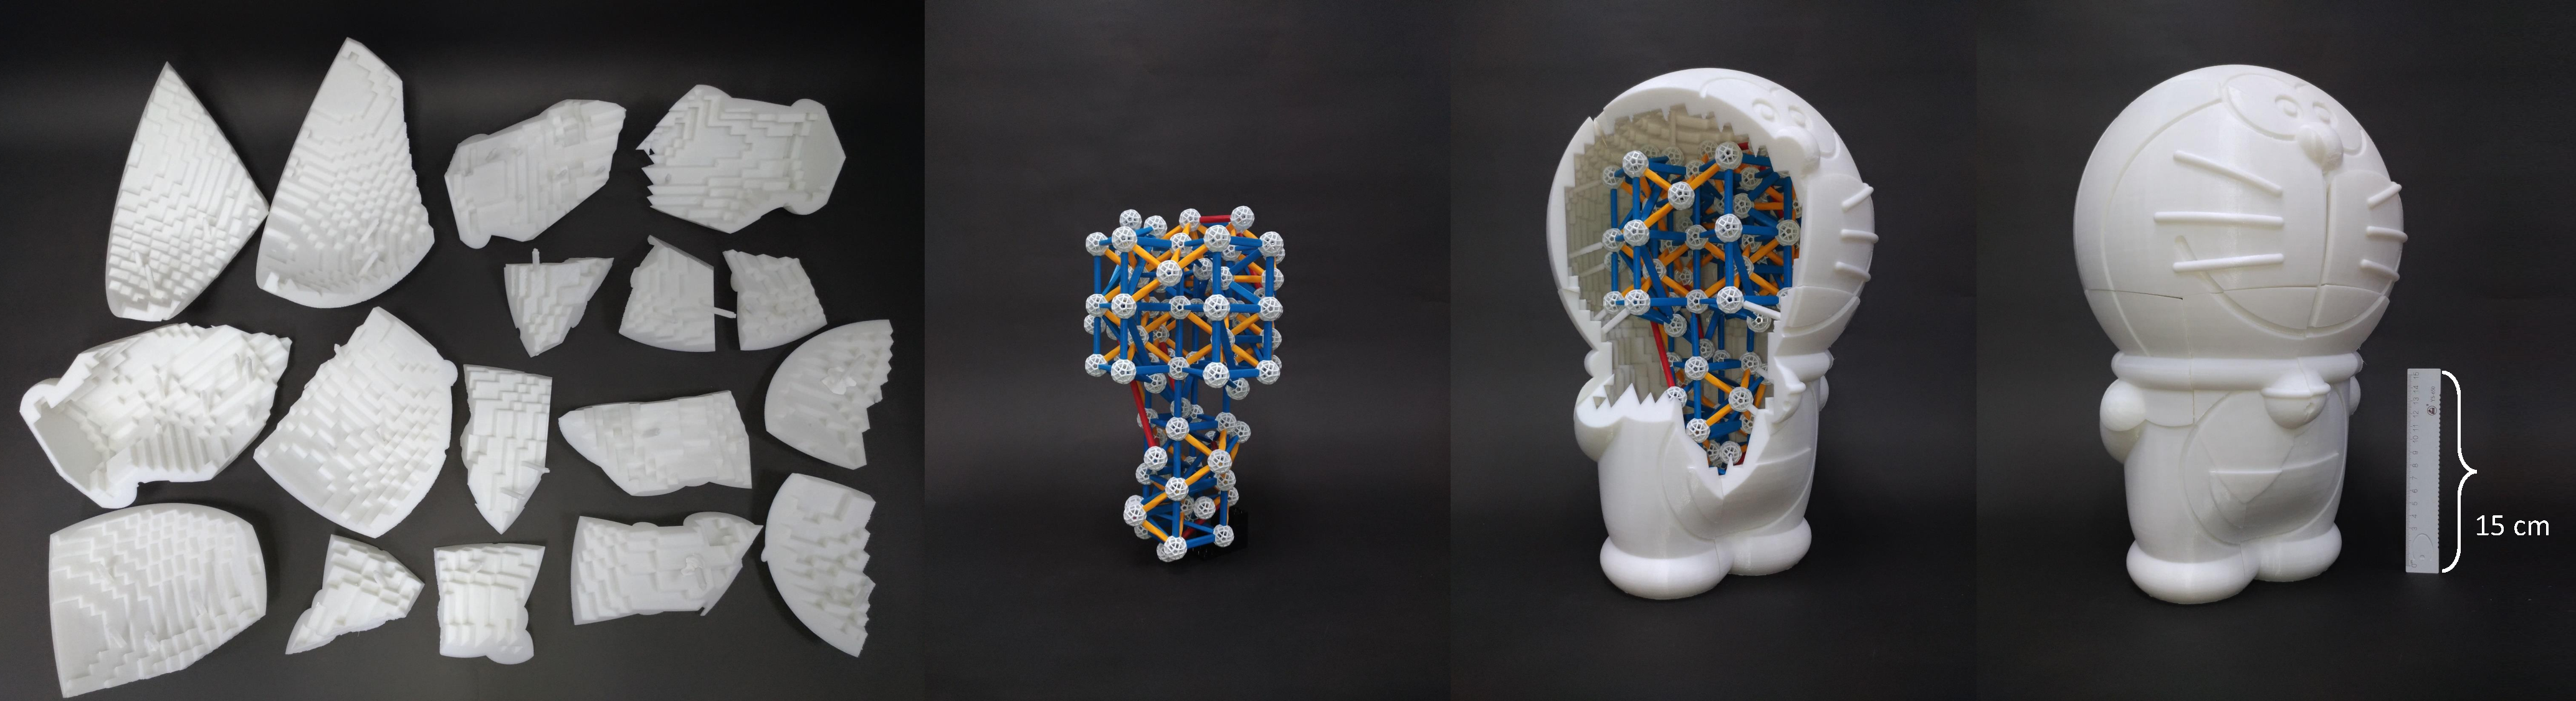
\includegraphics{figs/doraemon_real2.pdf}\\
% 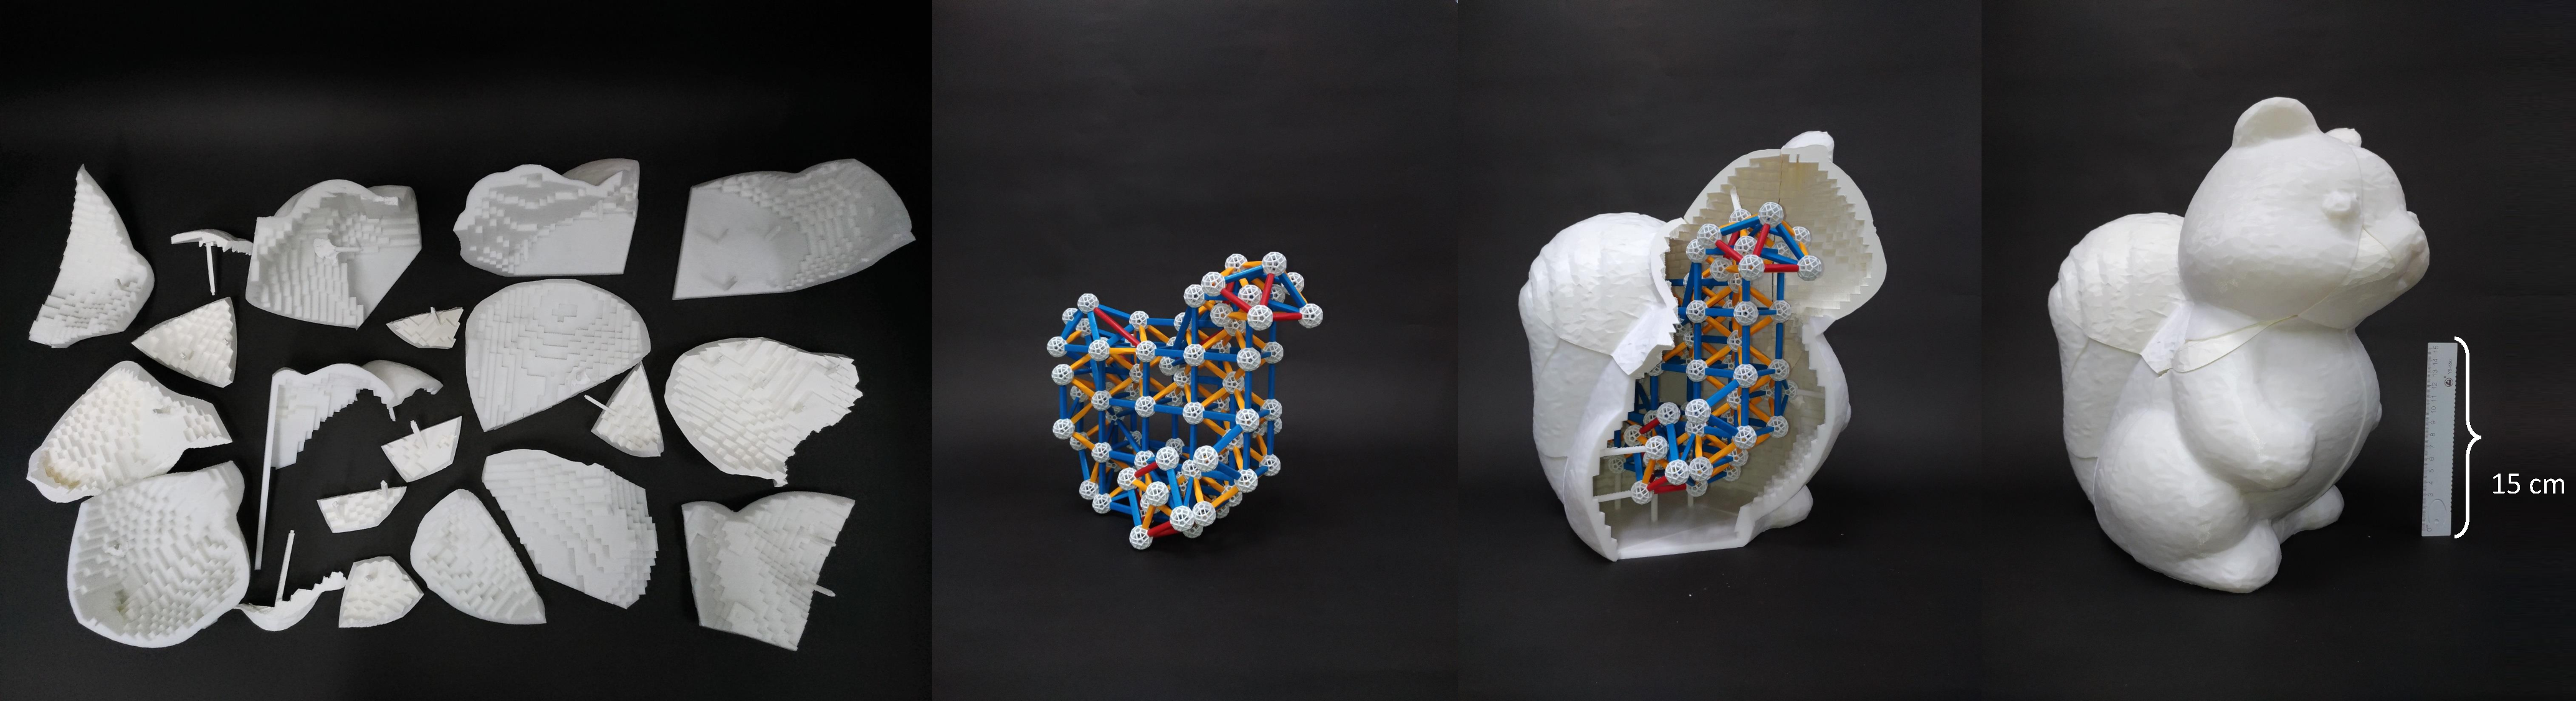
\includegraphics{figs/Squirrel_real2.pdf}\\
% 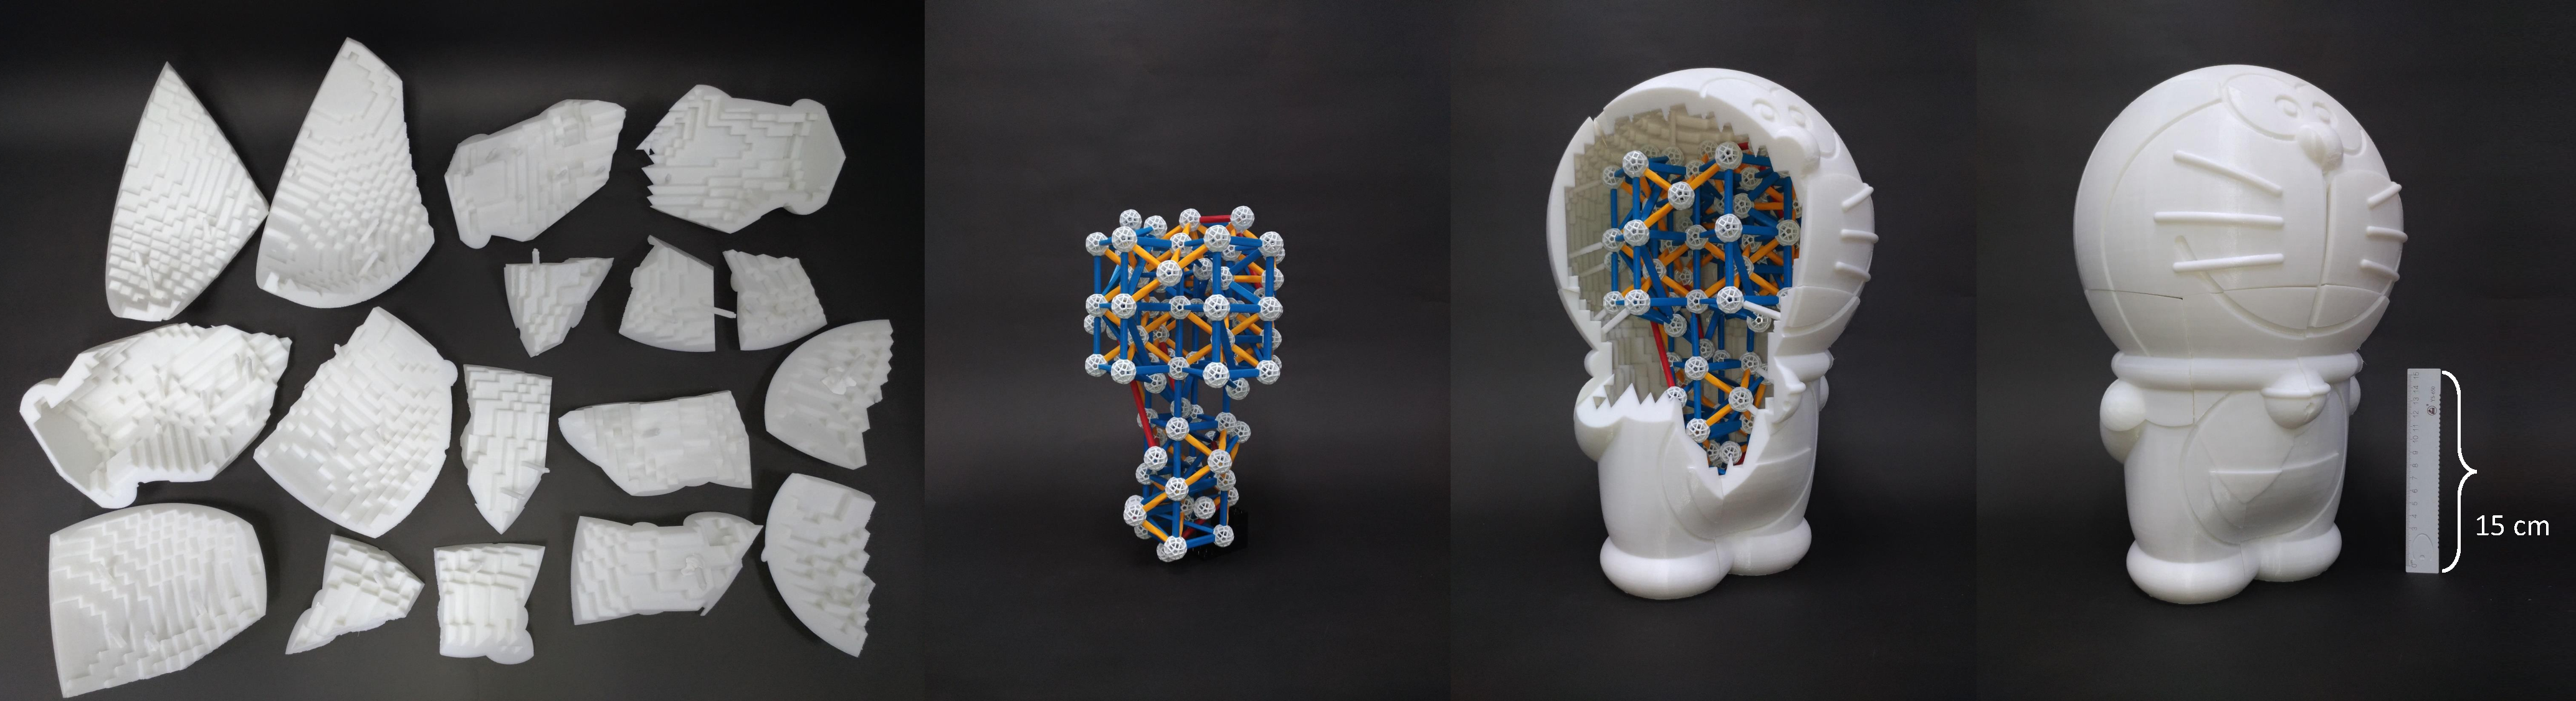
\includegraphics{figs/doraemon_real2.pdf}\\
% \end{tabular}
% }
% \caption{}
% \label{tab:result_ZomeFab_real}
% \end{table*}

\begin{table*}[ht]
\centering
\resizebox{0.965\linewidth}{!} {
\begin{tabular}{c} 
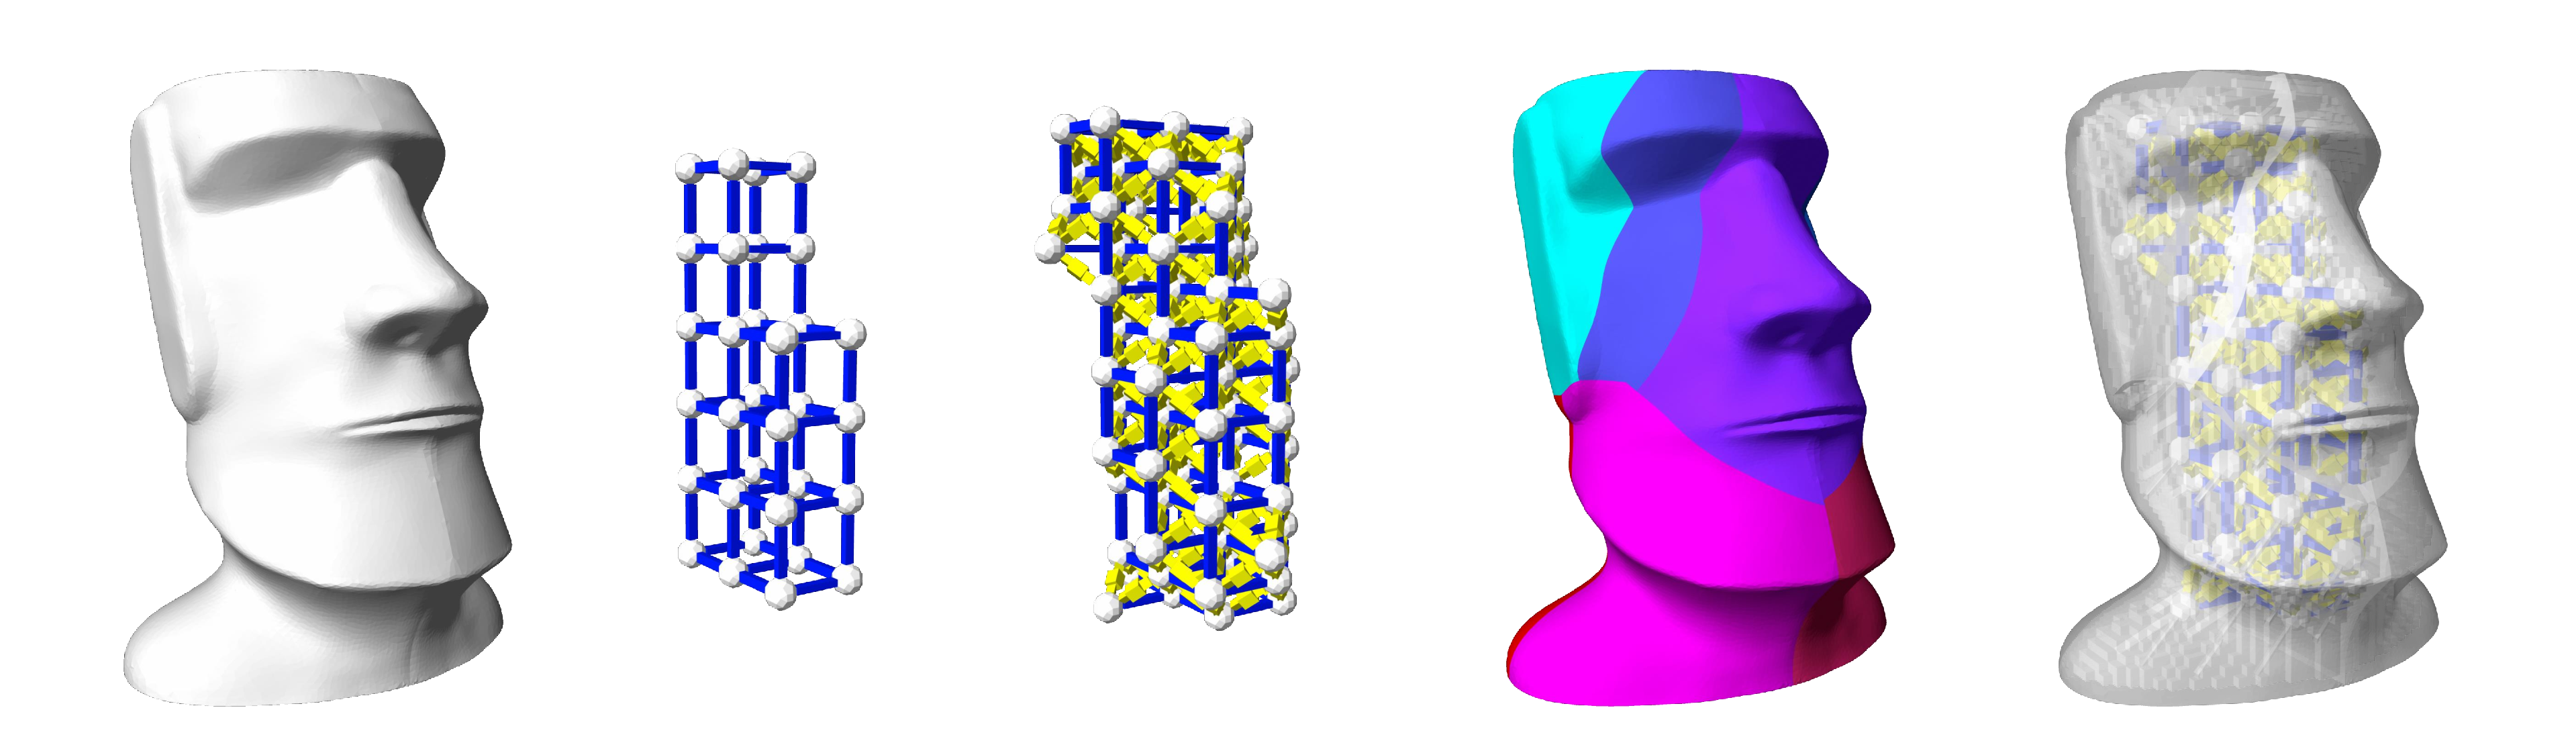
\includegraphics{figs/MOAI.pdf} \\
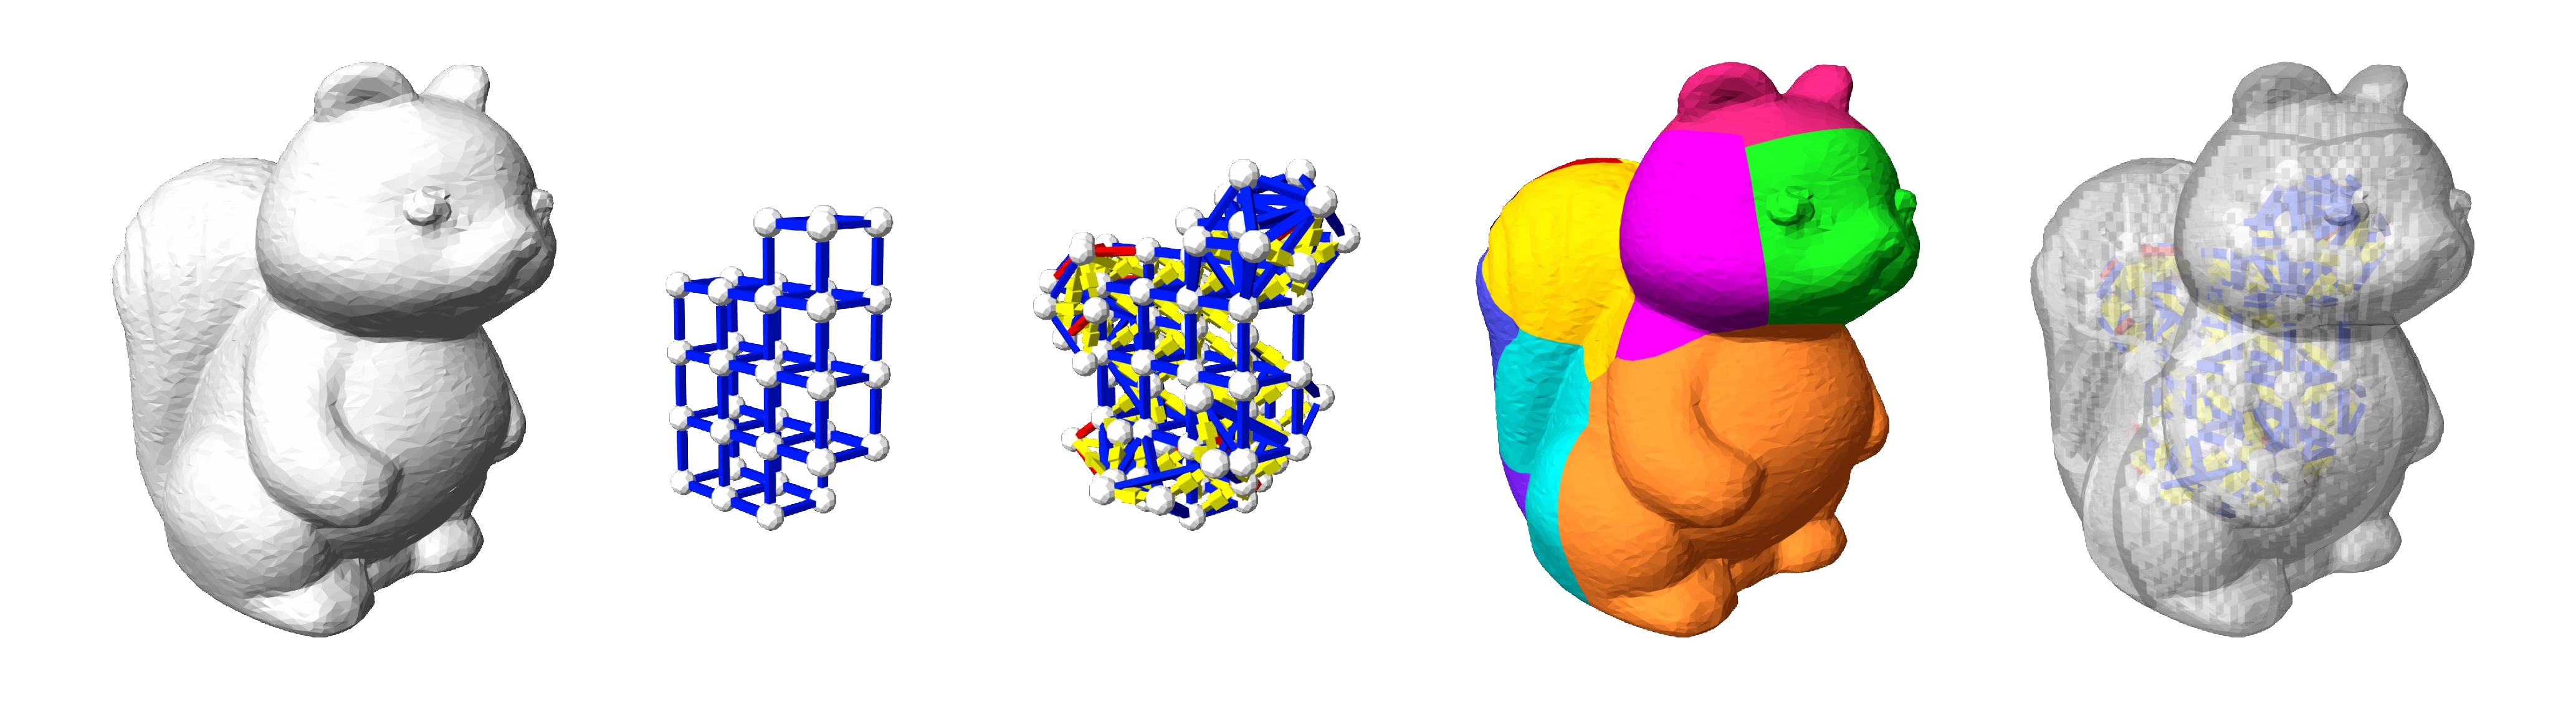
\includegraphics{figs/Squirrel.pdf}\\
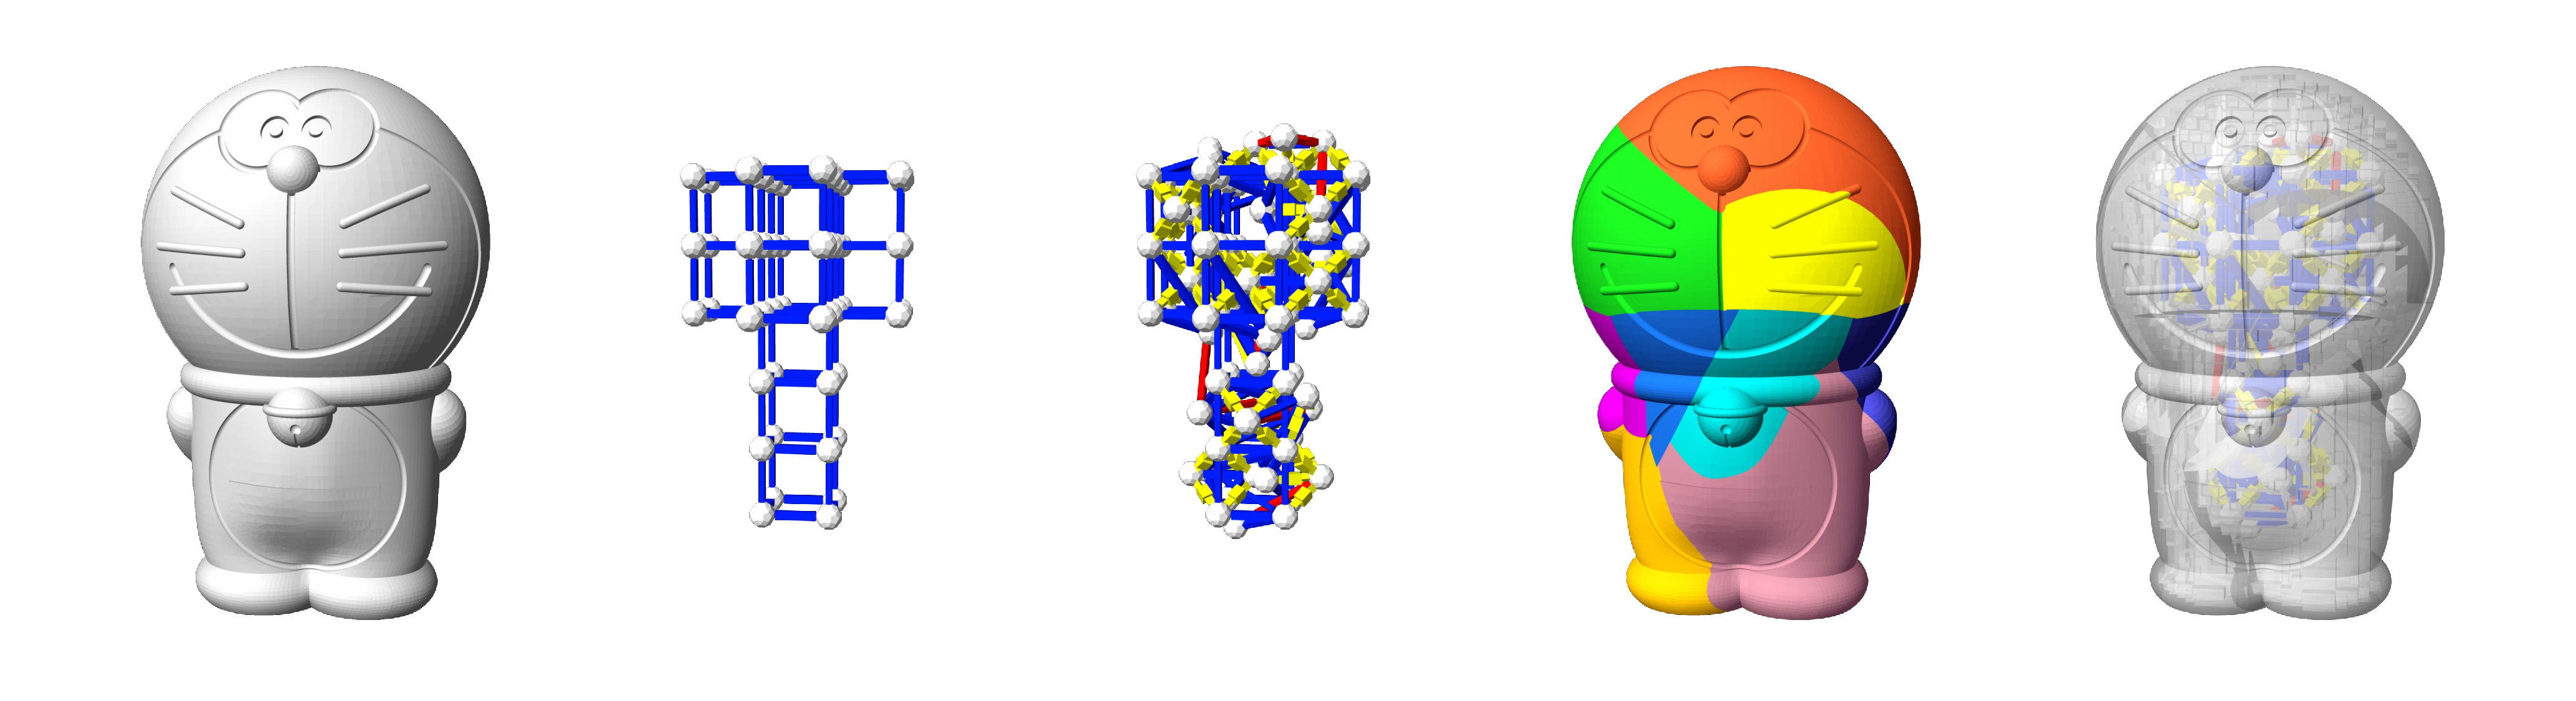
\includegraphics{figs/doraemon.pdf} \\
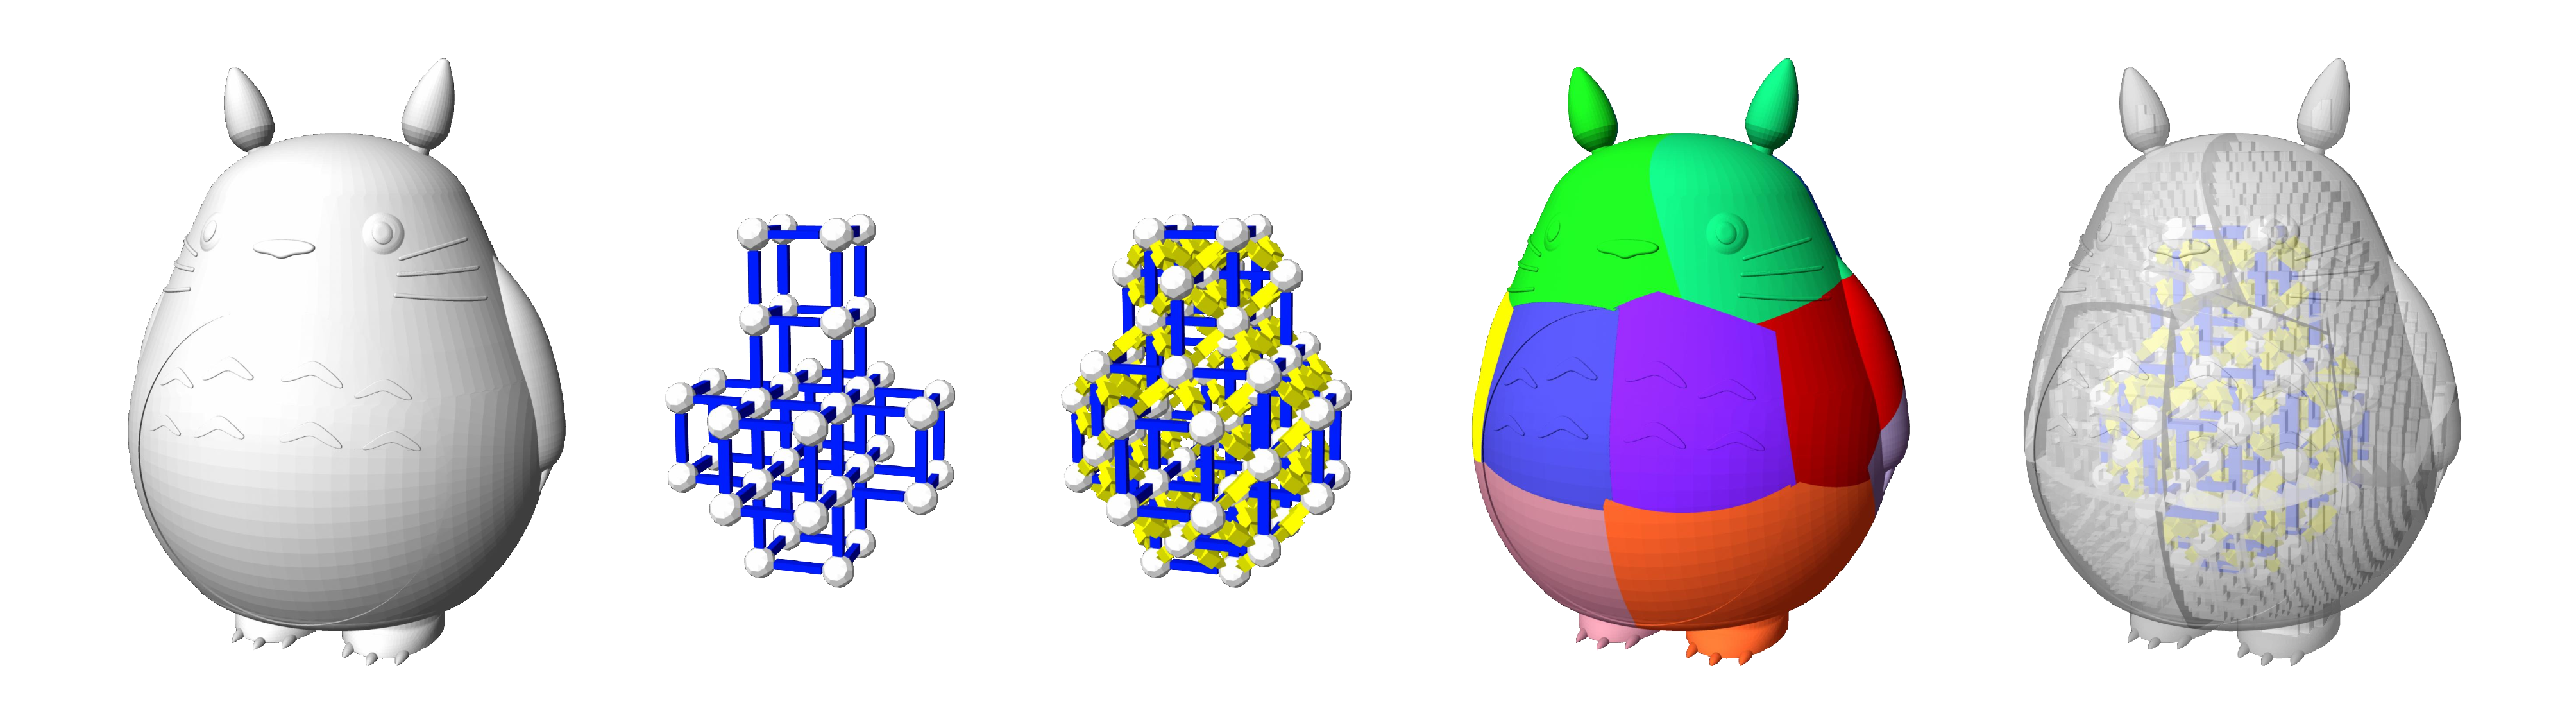
\includegraphics{figs/totoro.pdf}\\
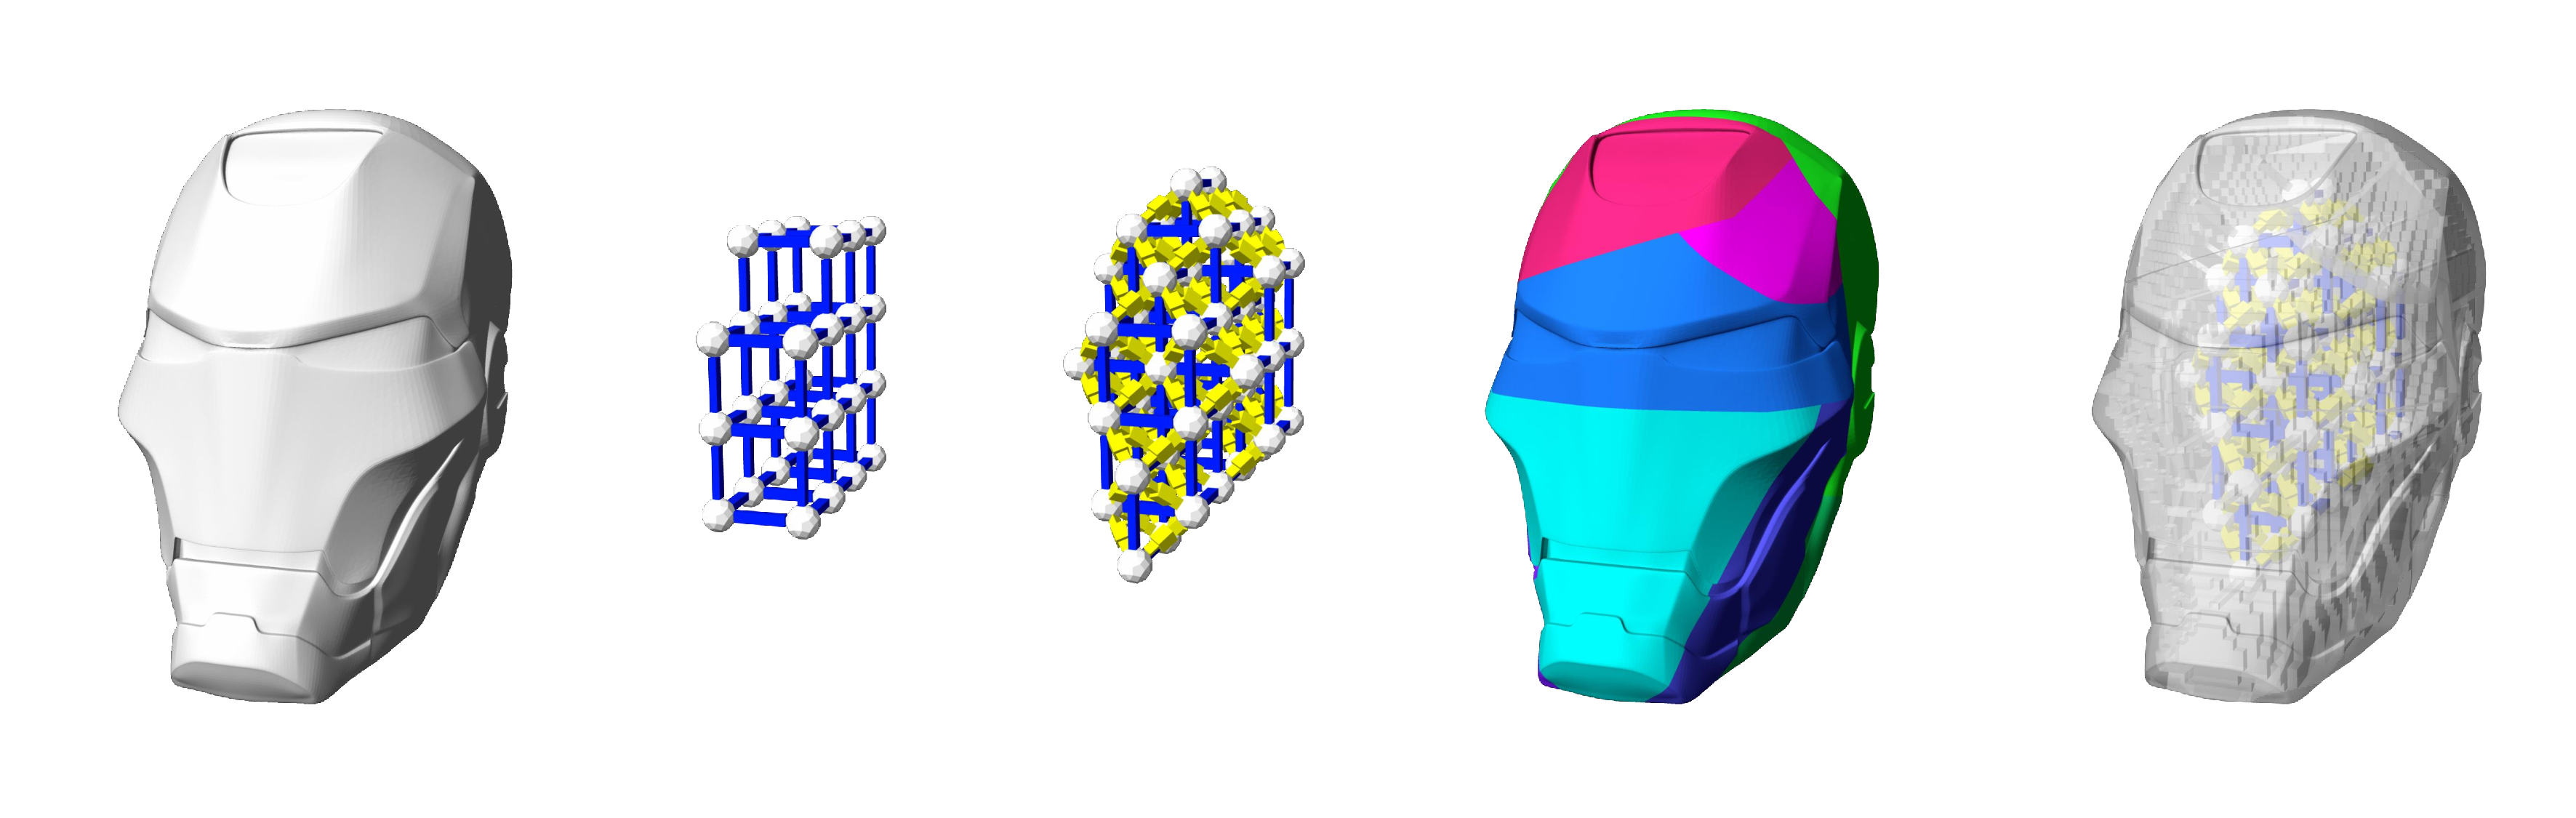
\includegraphics{figs/iron.pdf}\\
\end{tabular}
}
\caption{}
\label{tab:result_ZomeFab_file_1}
\end{table*}

\begin{table*}[ht]
\centering
\resizebox{1.\linewidth}{!} {
\begin{tabular}{c} 
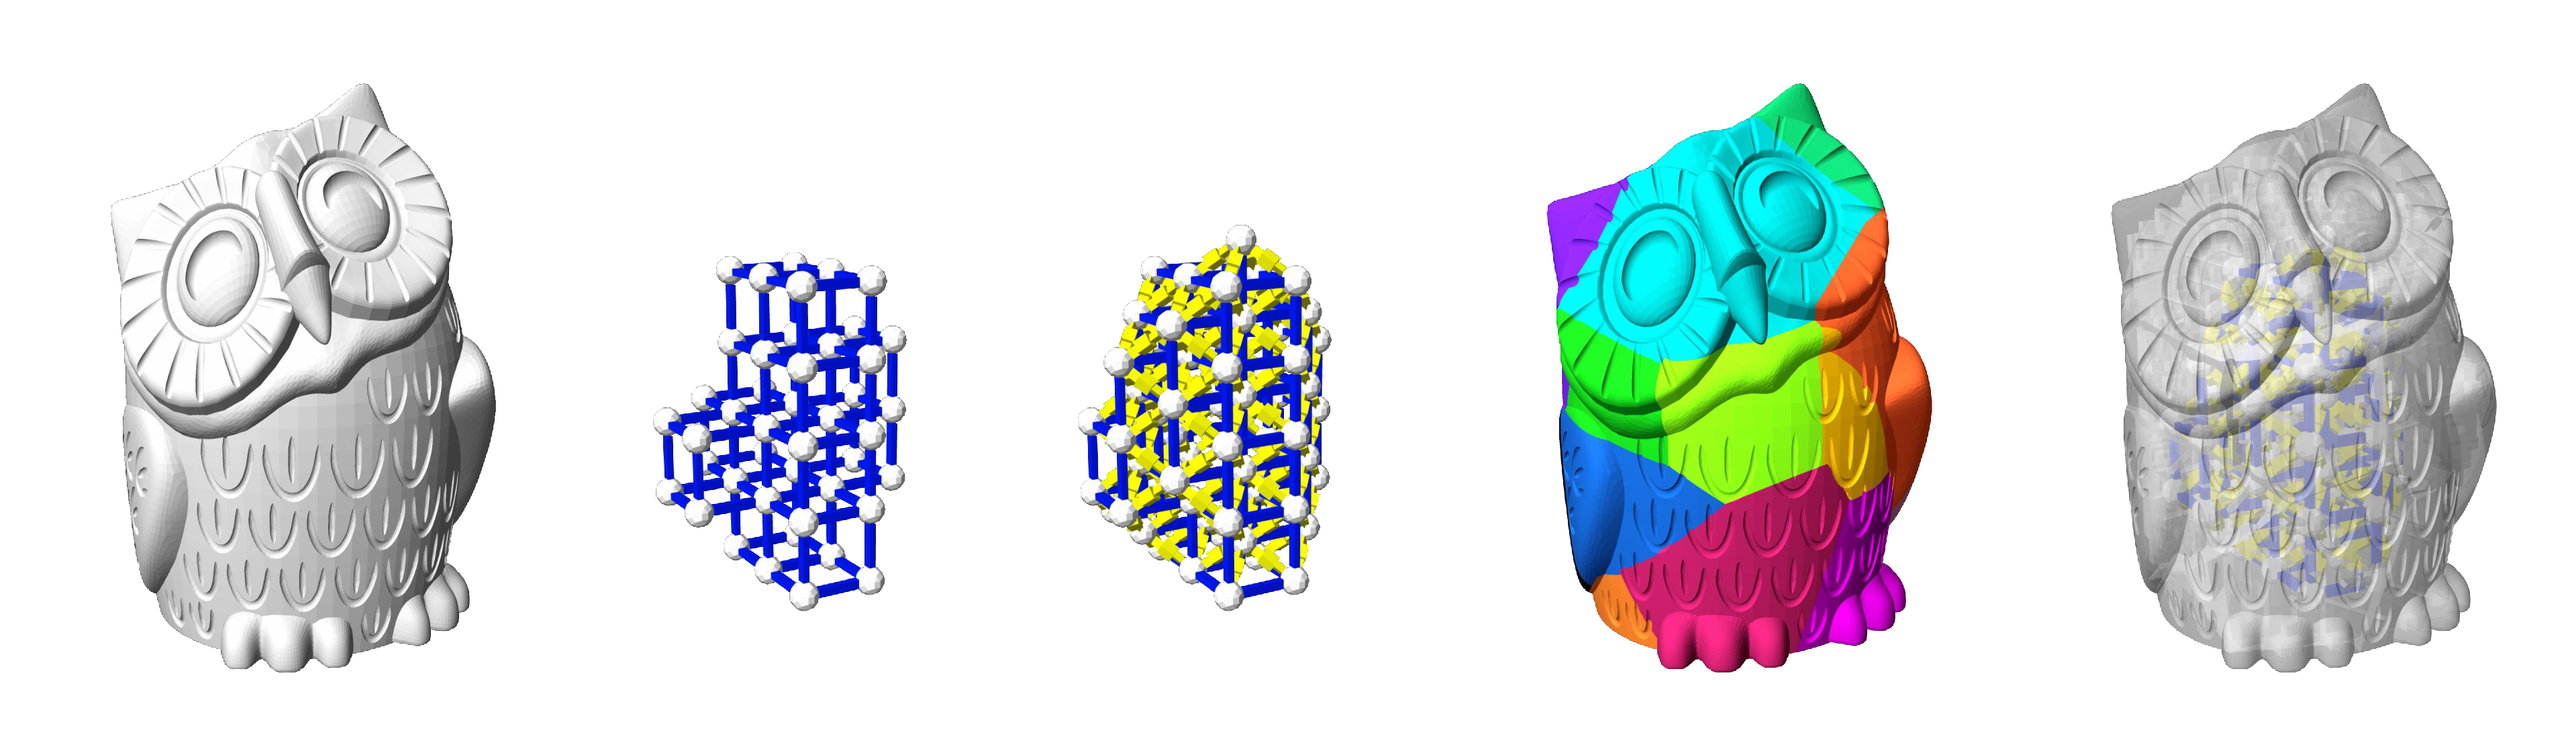
\includegraphics{figs/owl.pdf}\\
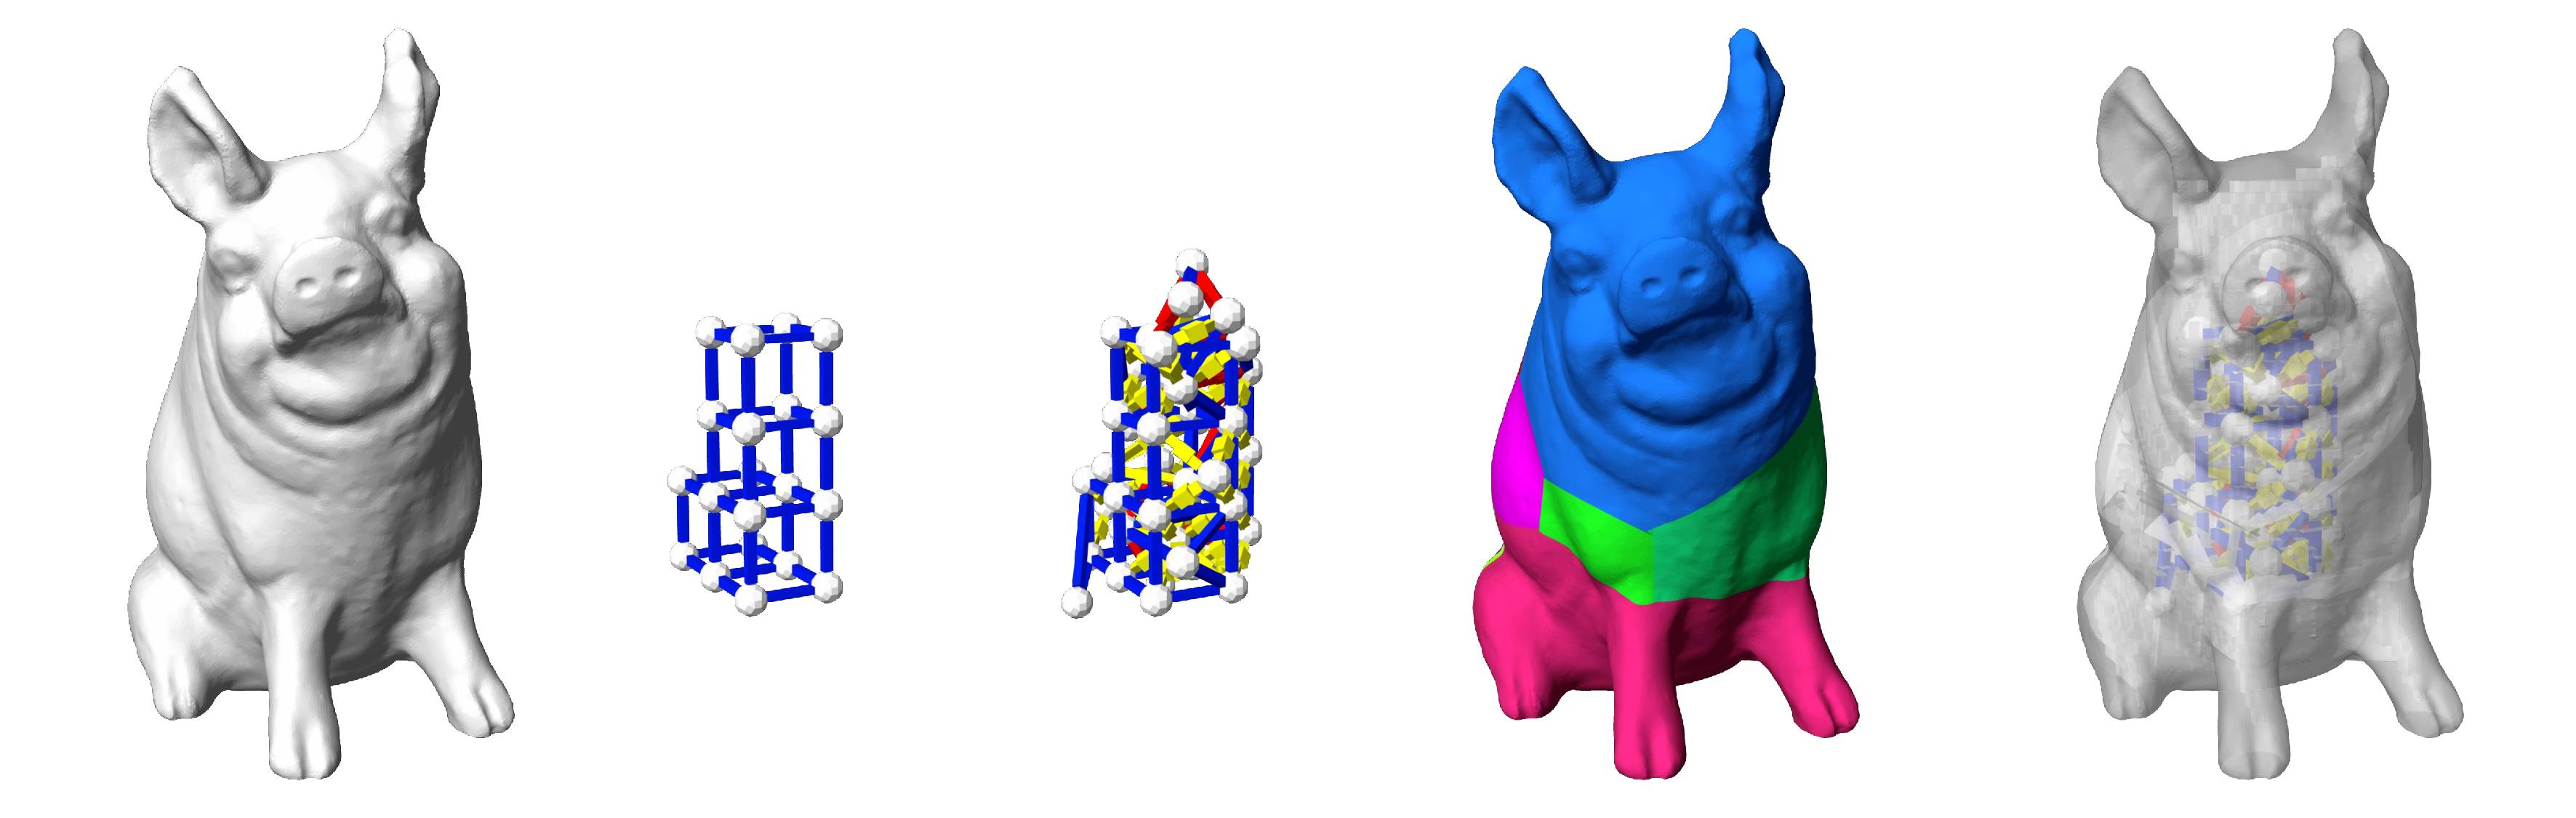
\includegraphics{figs/pig.pdf} \\
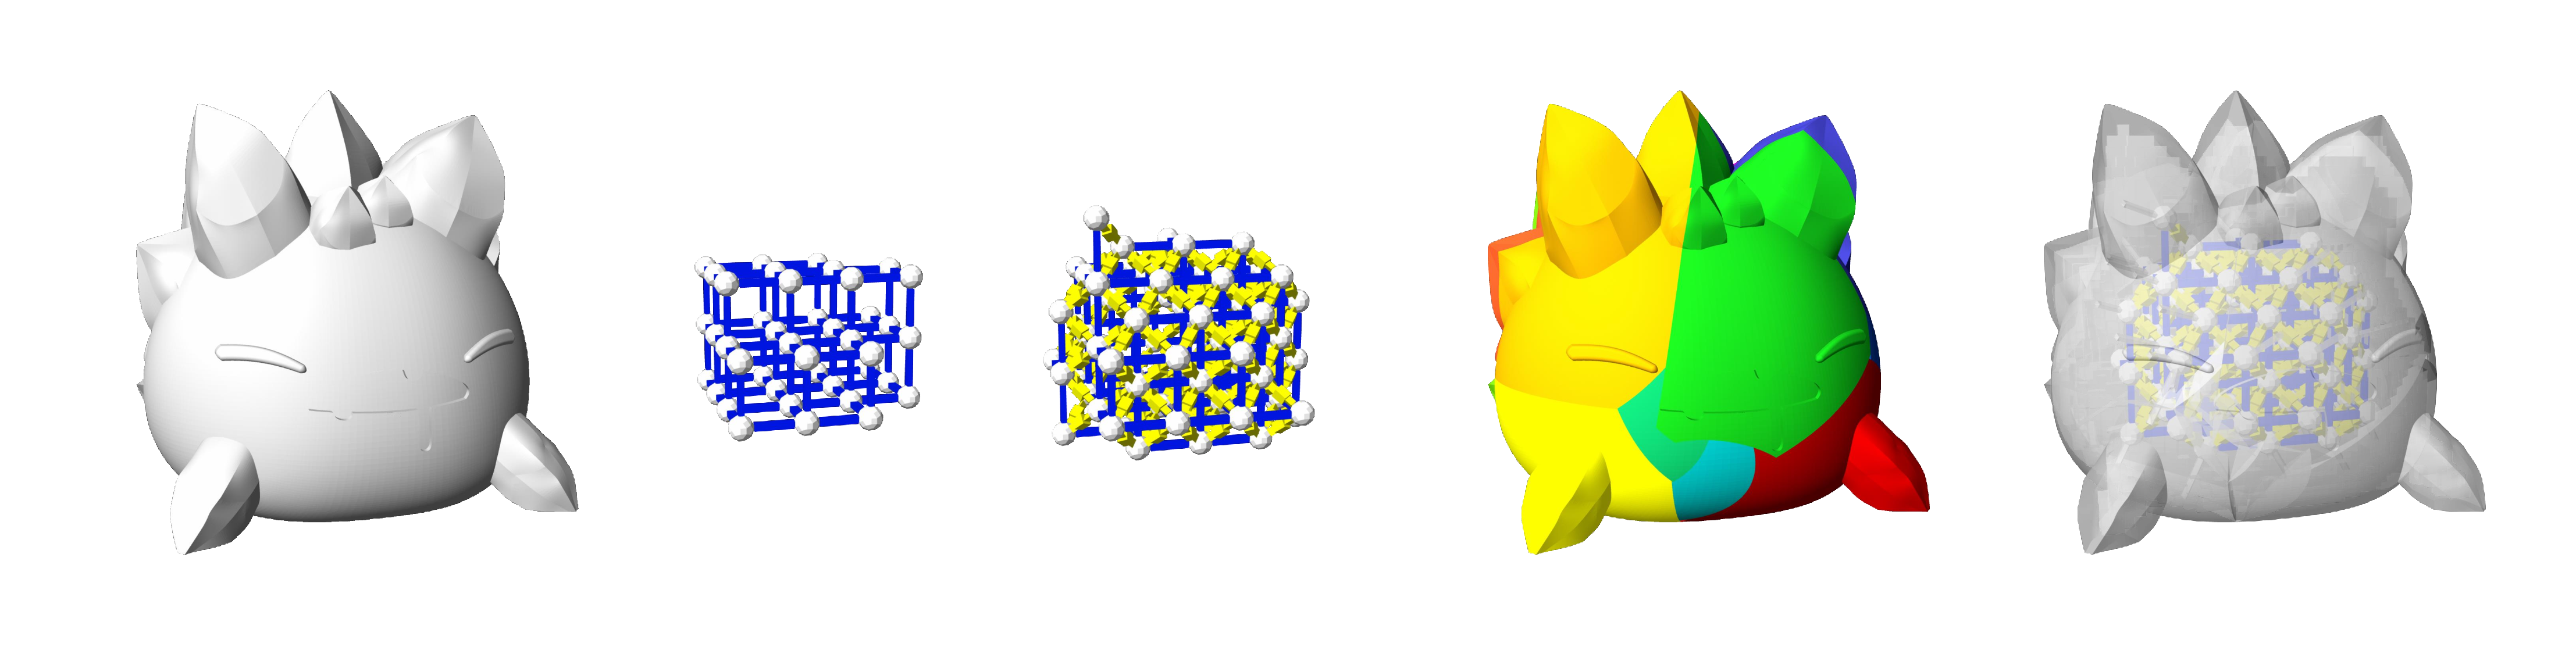
\includegraphics{figs/slime_high.pdf}\\
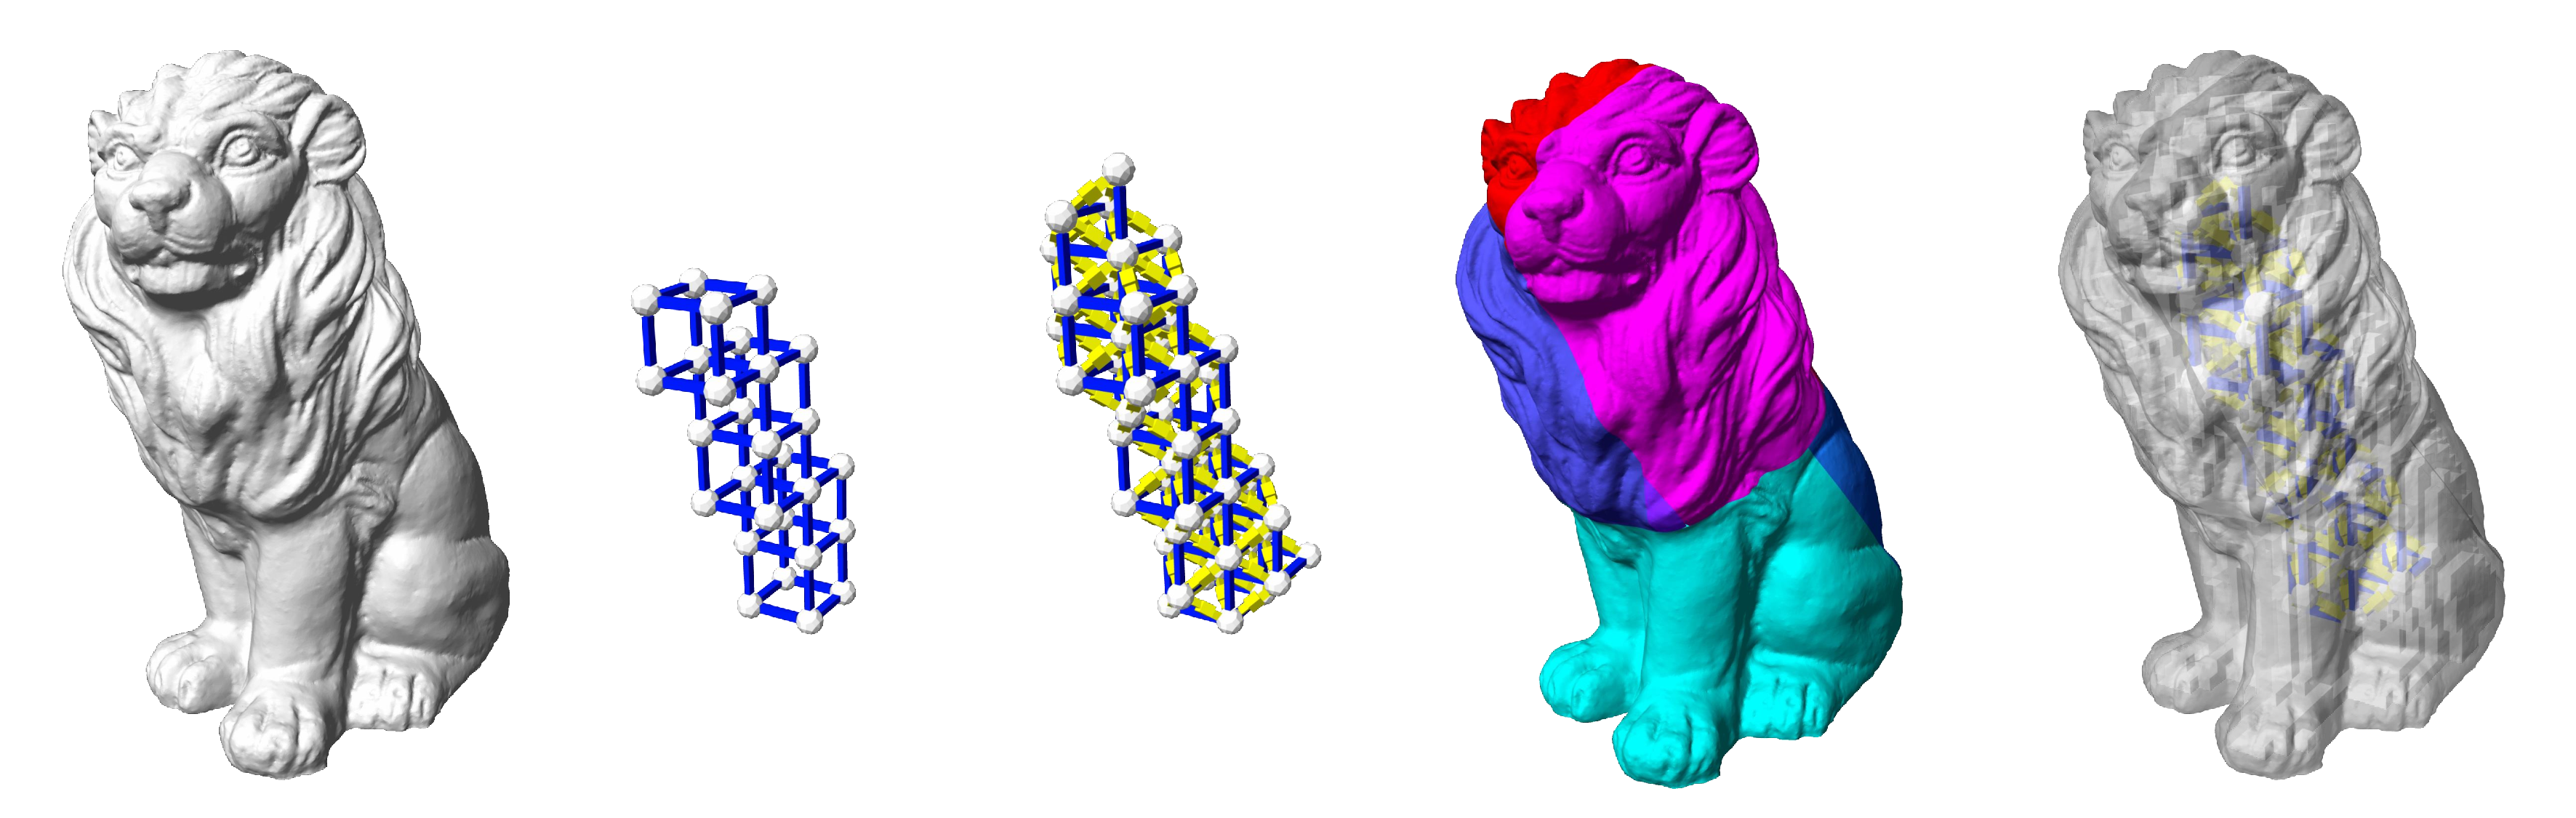
\includegraphics{figs/lion.pdf}\\
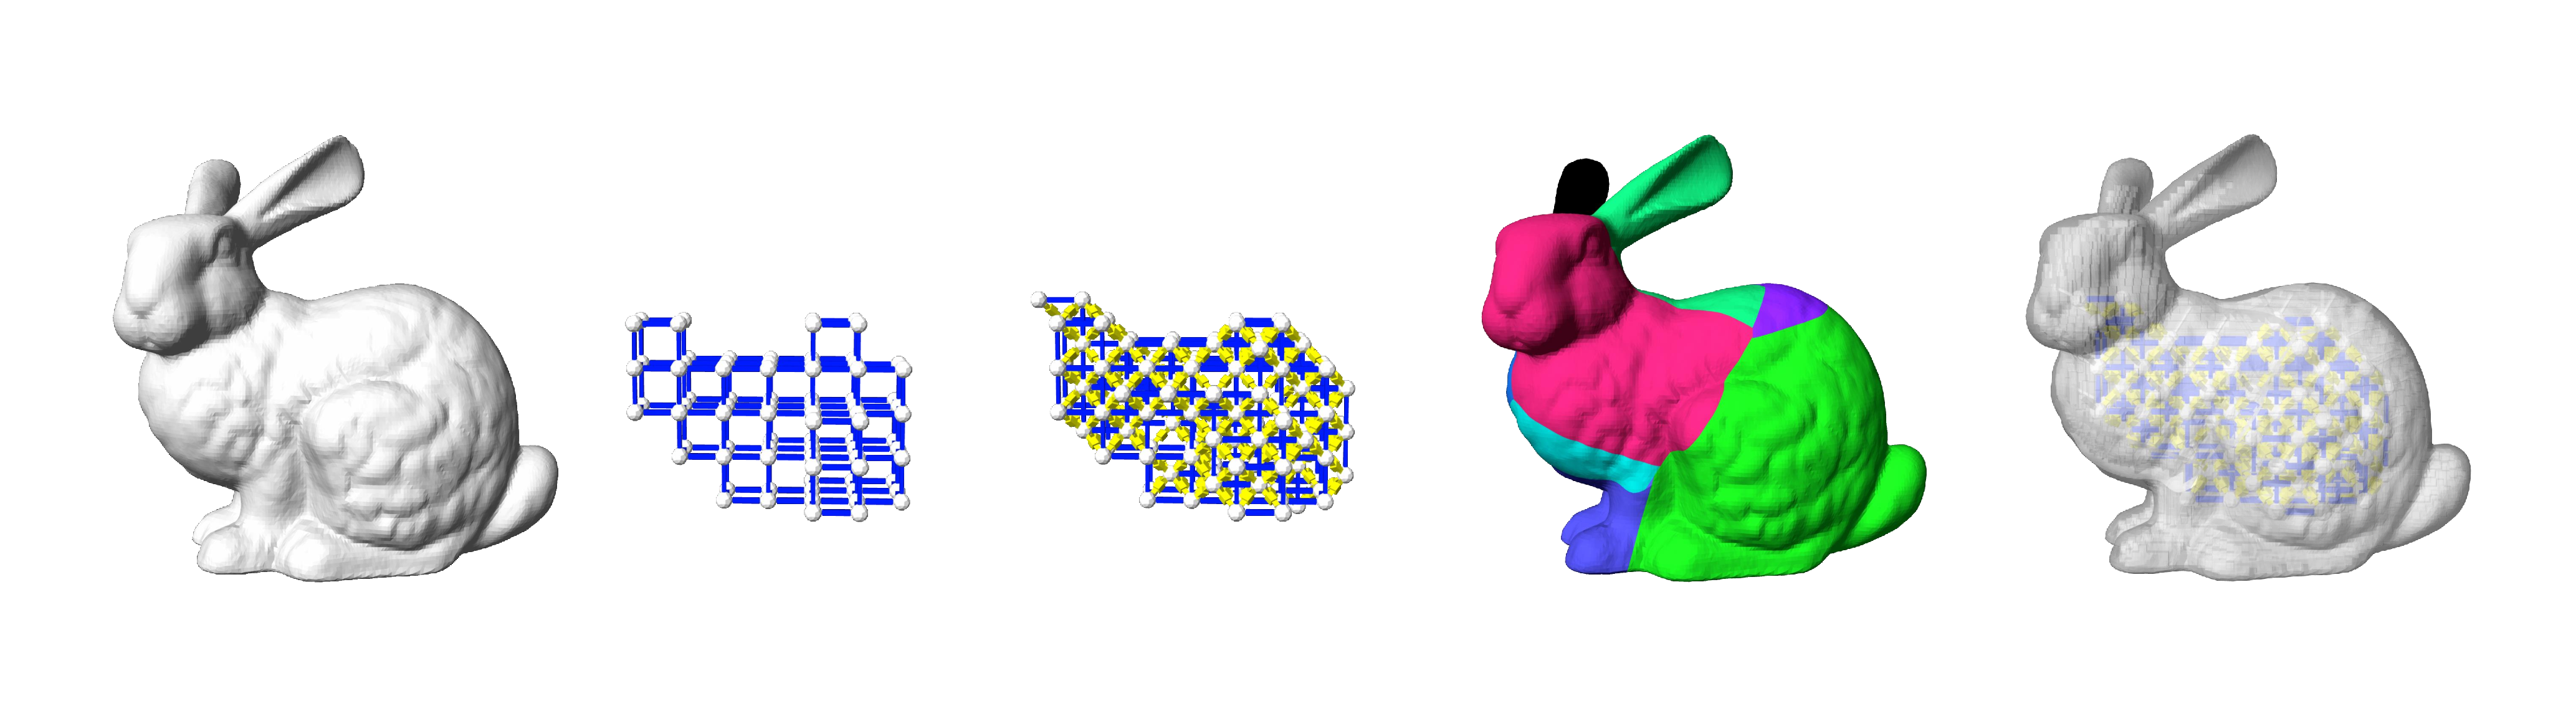
\includegraphics{figs/bunny_150.pdf}\\
\end{tabular}
}
\caption{}
\label{tab:result_ZomeFab_file_2}
\end{table*}

%\begin{figure*}[ht]
%\centering
%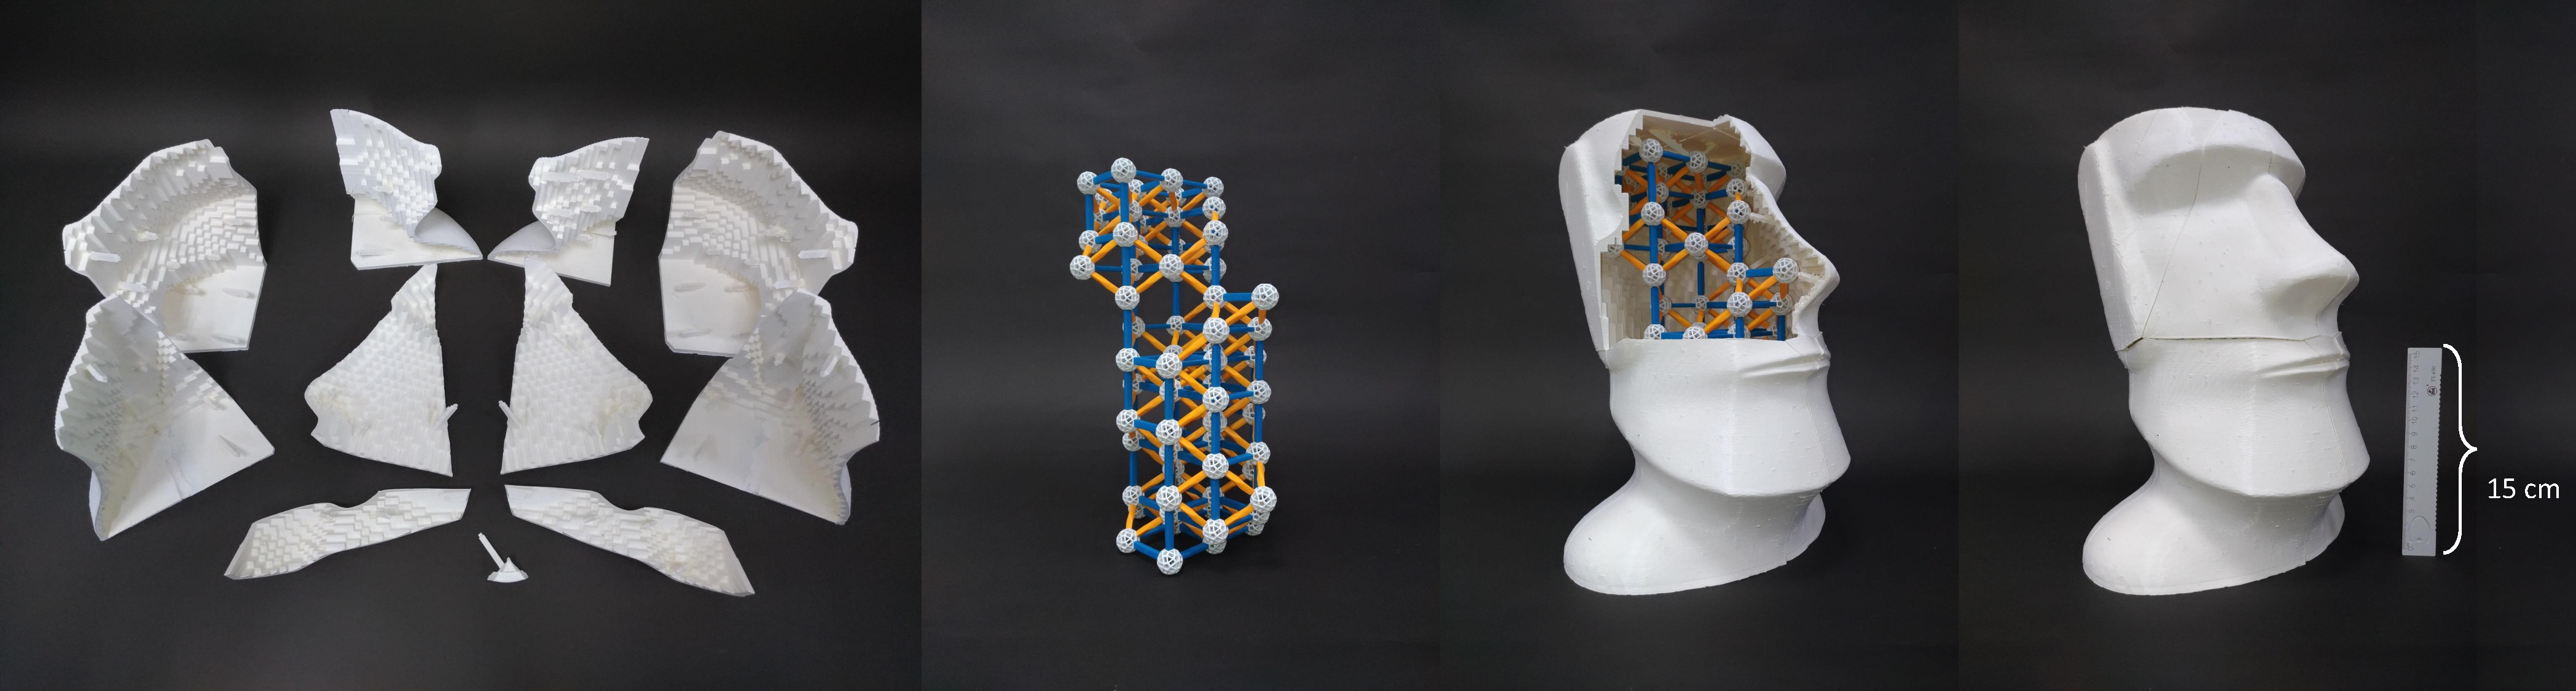
\includegraphics[width=1.0\linewidth]{figs/MOAI_real2.pdf}
%\caption{Result fabricated and assembly : Moai}
%\label{fig:result-assembly_Moai_real}
%\end{figure*}

%\begin{figure*}[ht]
%\centering
%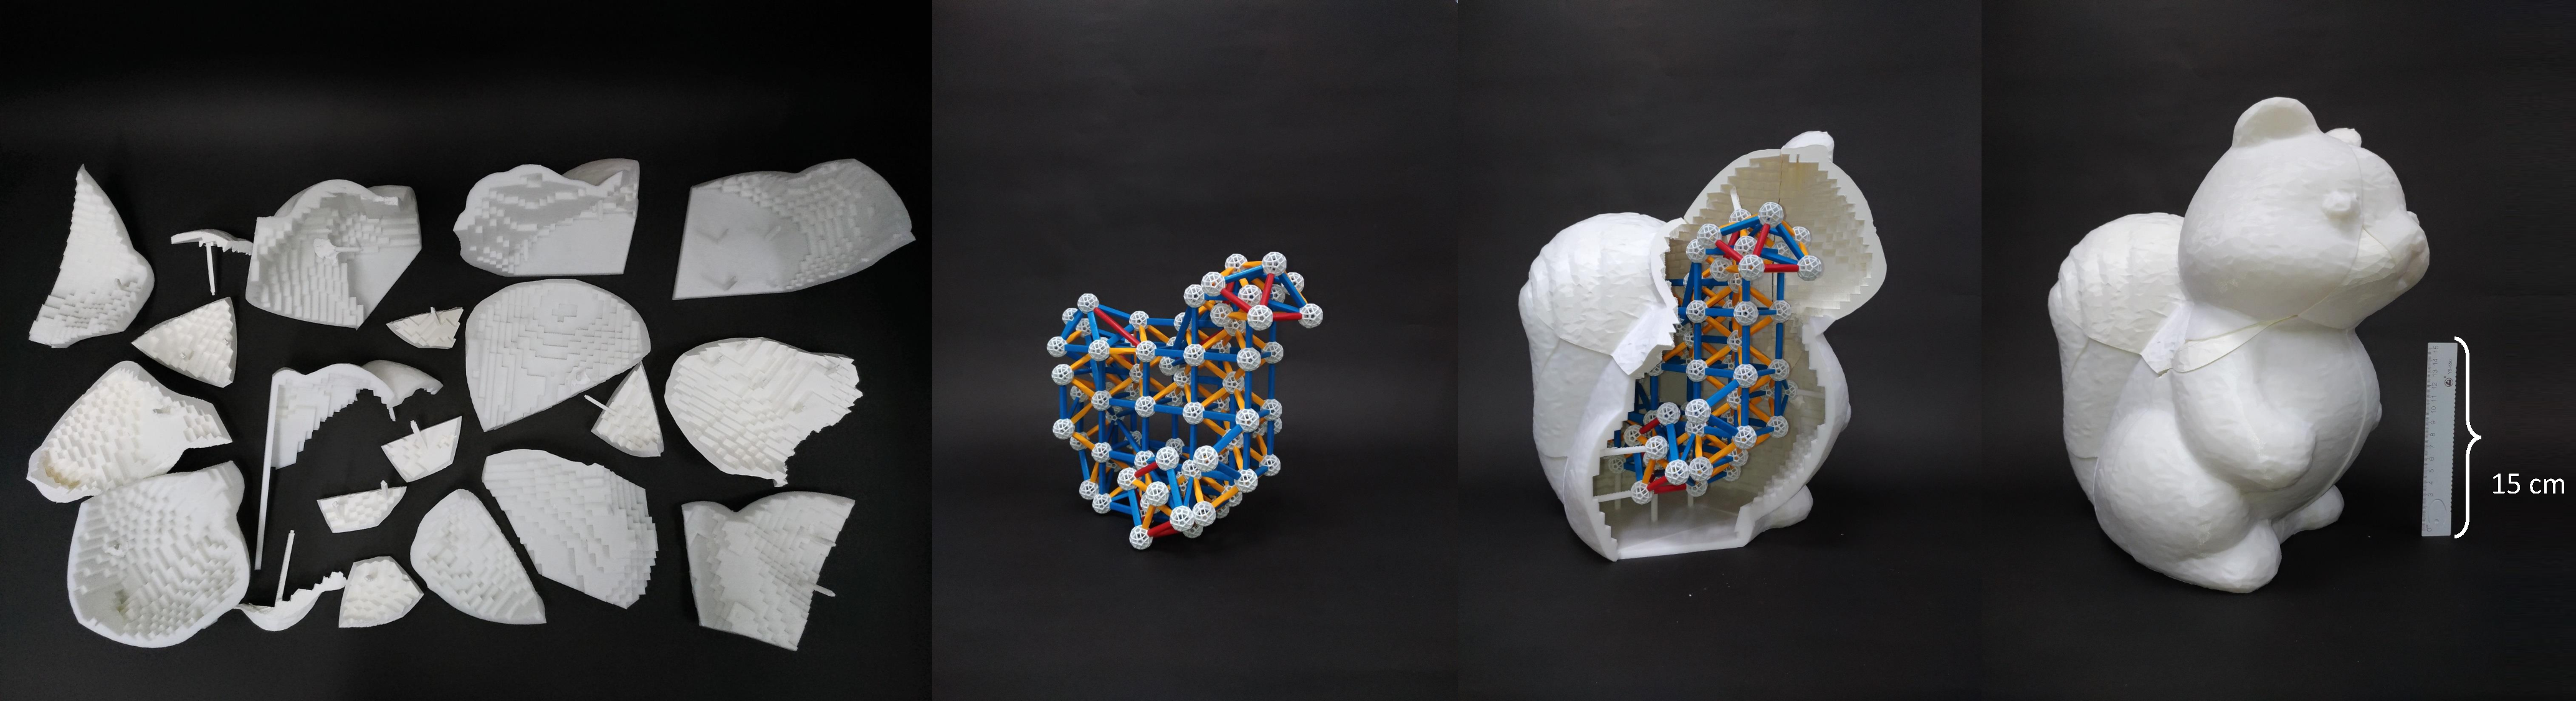
\includegraphics[width=1.0\linewidth]{figs/Squirrel_real2.pdf} 
%\caption{Result fabricated and assembly : Squirrel}
%\label{fig:result-assembly_Squirrel_real}
%\end{figure*}

%\begin{figure*}[ht]
%\centering
%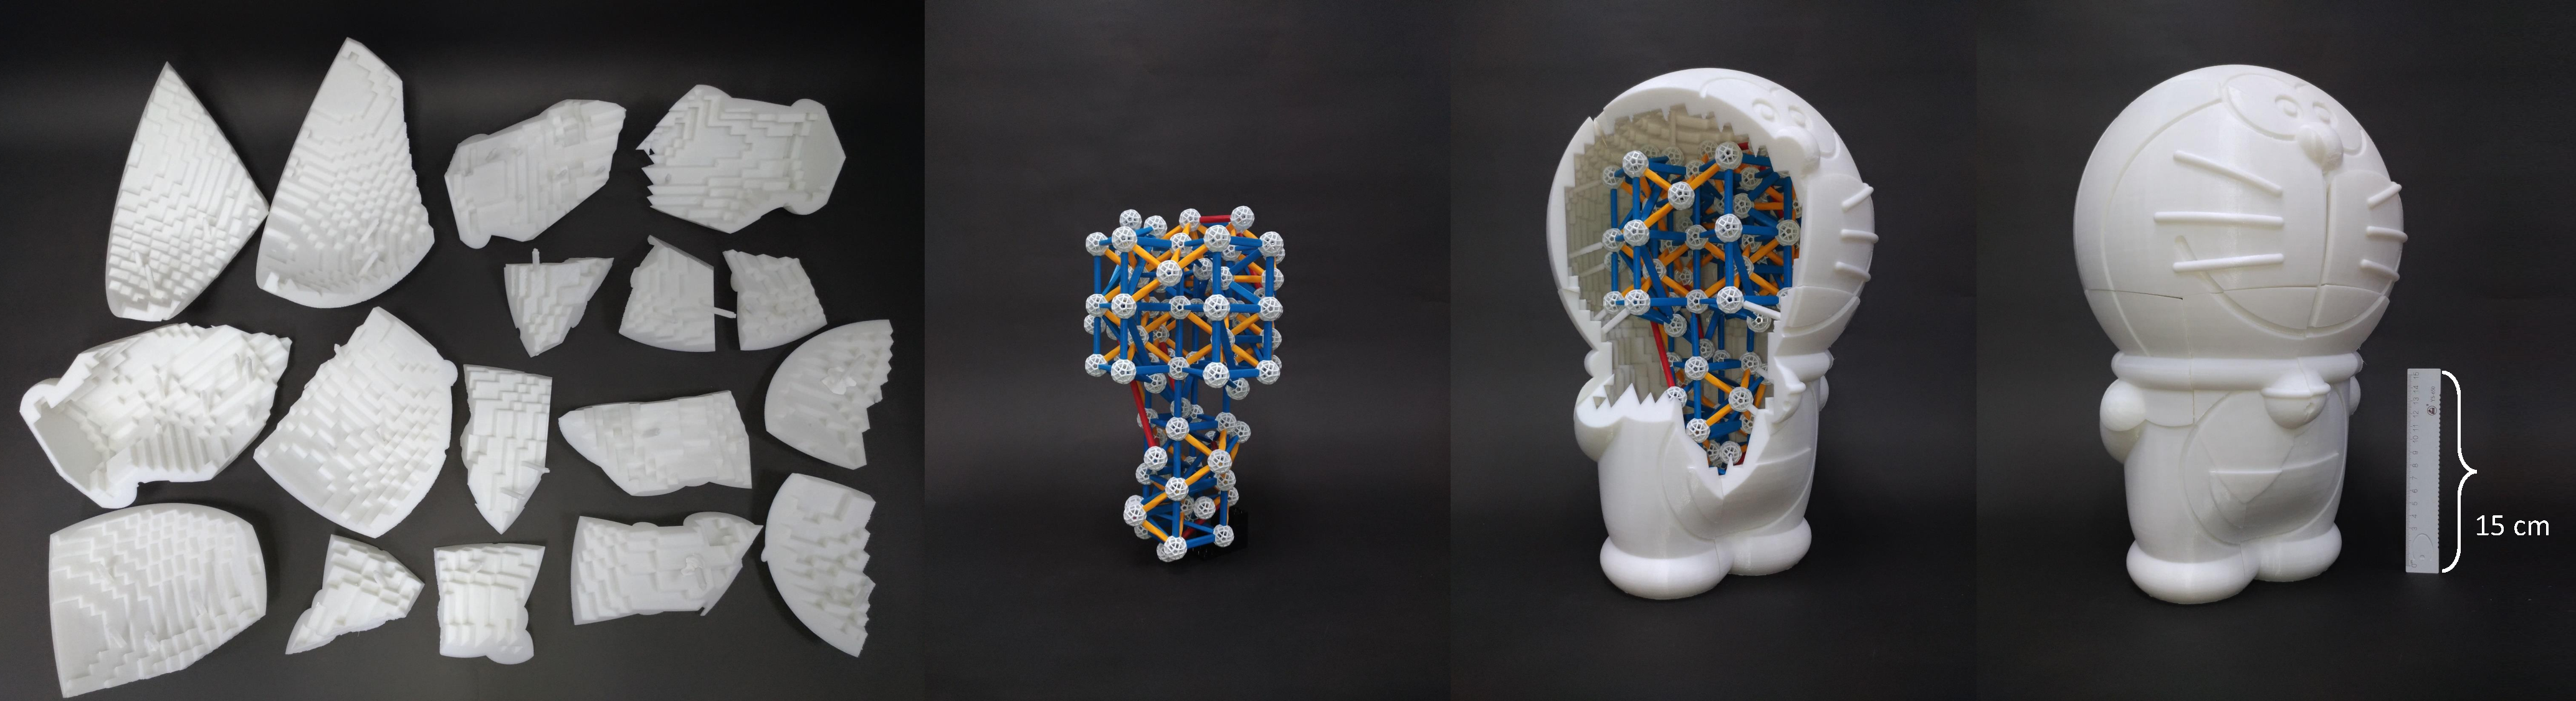
\includegraphics[width=1.0\linewidth]{figs/doraemon_real2.pdf} 
%\caption{Result fabricated and assembly : Doraemon}
%\label{fig:result-assembly_doraemon_real}
%\end{figure*}

%\begin{figure*}[ht]
%\centering
%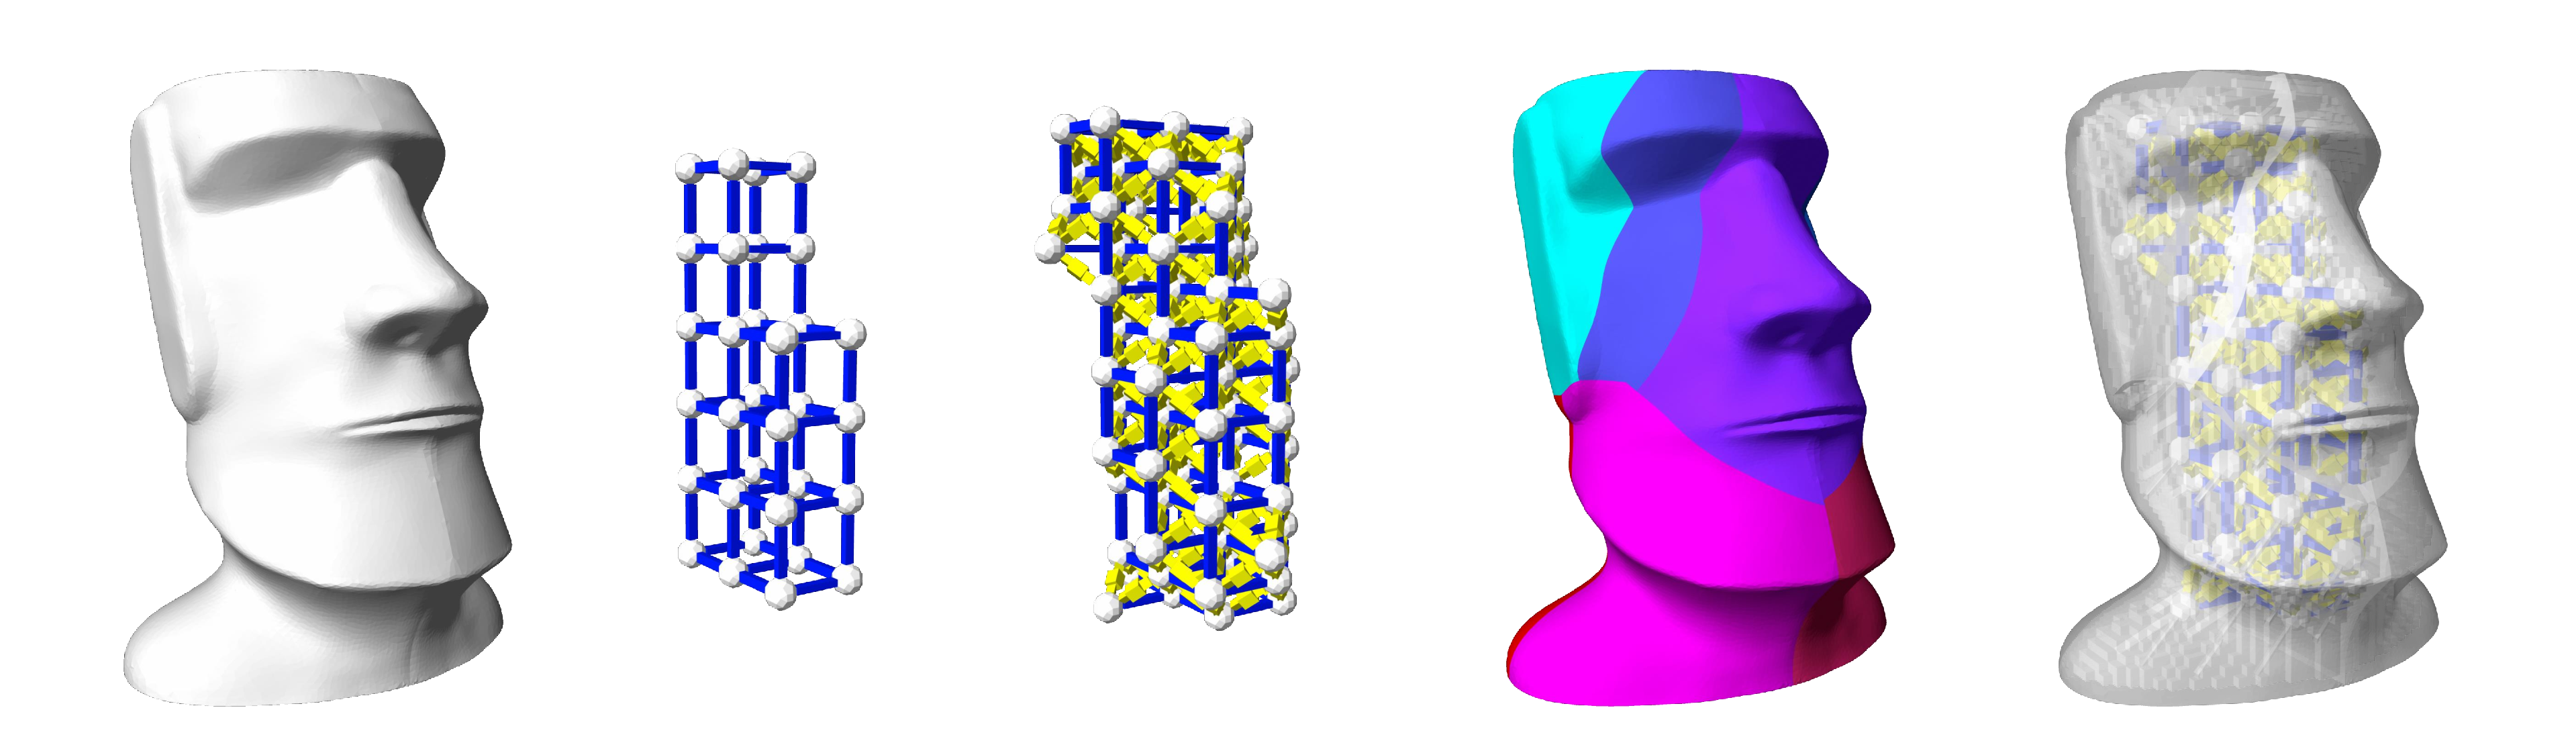
\includegraphics[width=1.0\linewidth]{figs/MOAI.pdf} 
%\caption{Result : MOAI}
%\label{fig:result-assembly_MOAI}
%\end{figure*}

%\begin{figure*}[ht]
%\centering
%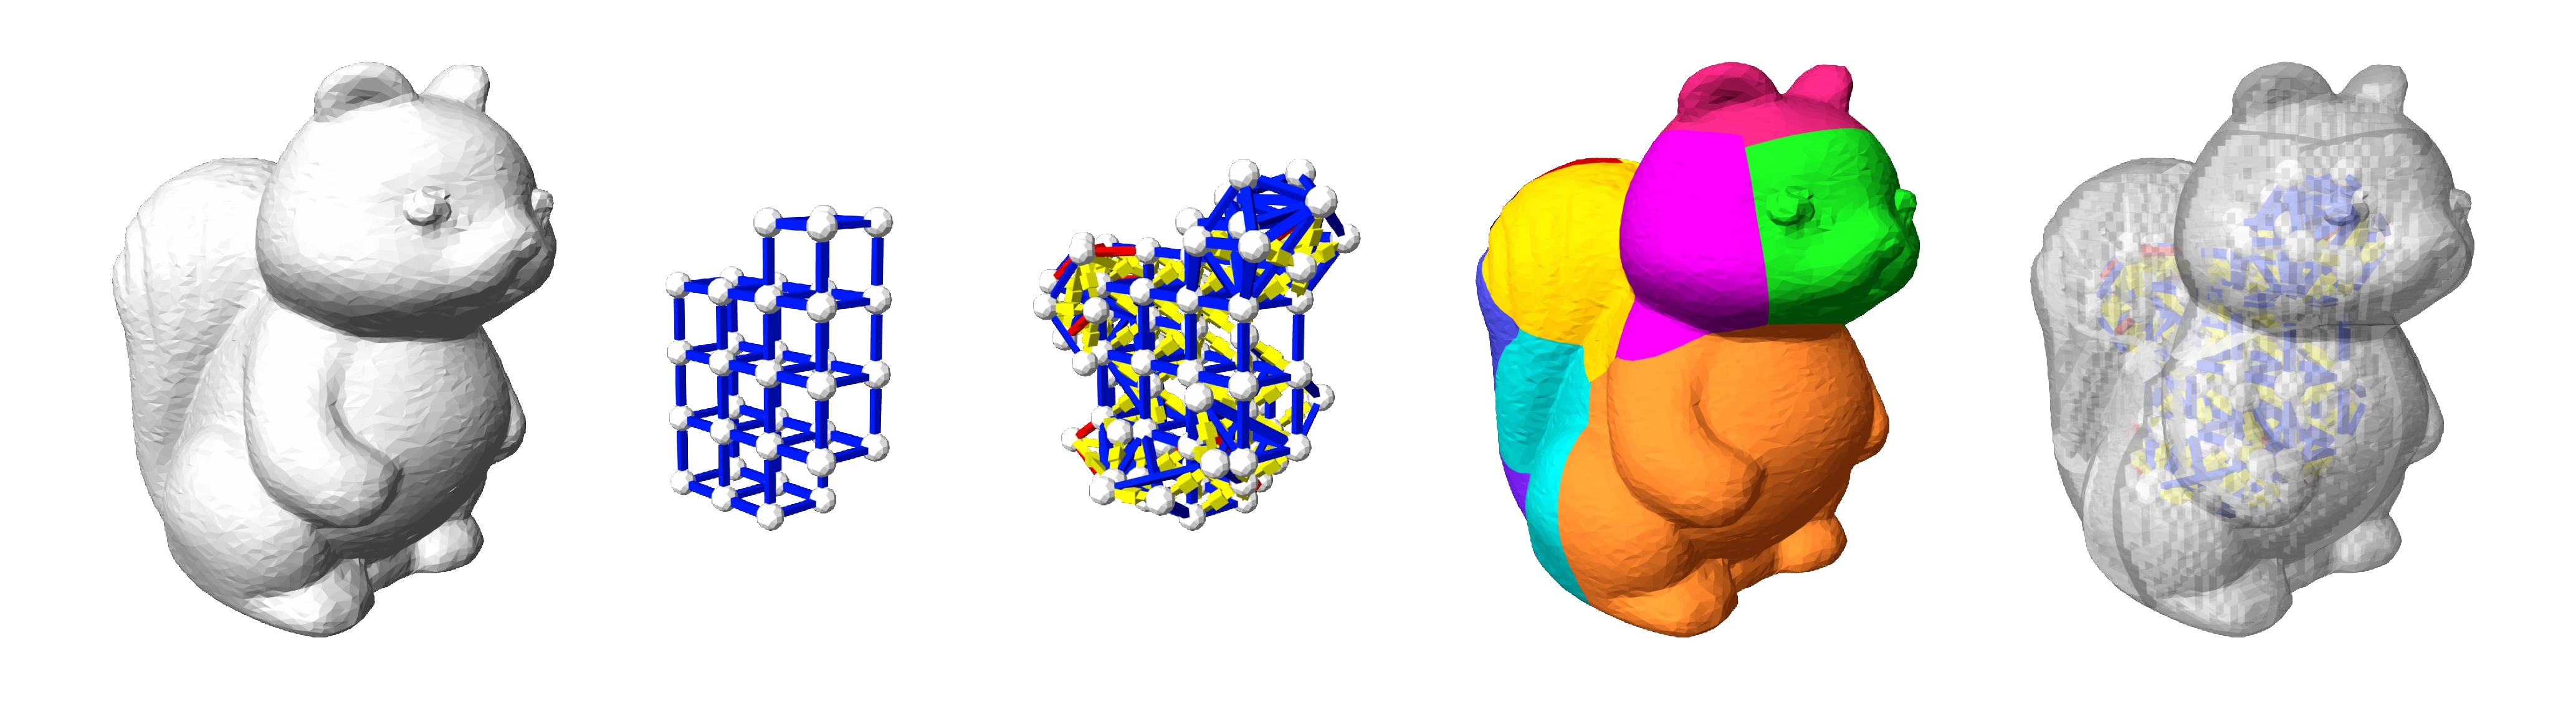
\includegraphics[width=1.0\linewidth]{figs/Squirrel.pdf} 
%\caption{Result : Squirrel}
%\label{fig:result-assembly_Squirrel}
%\end{figure*}

%\begin{figure*}[ht]
%\centering
%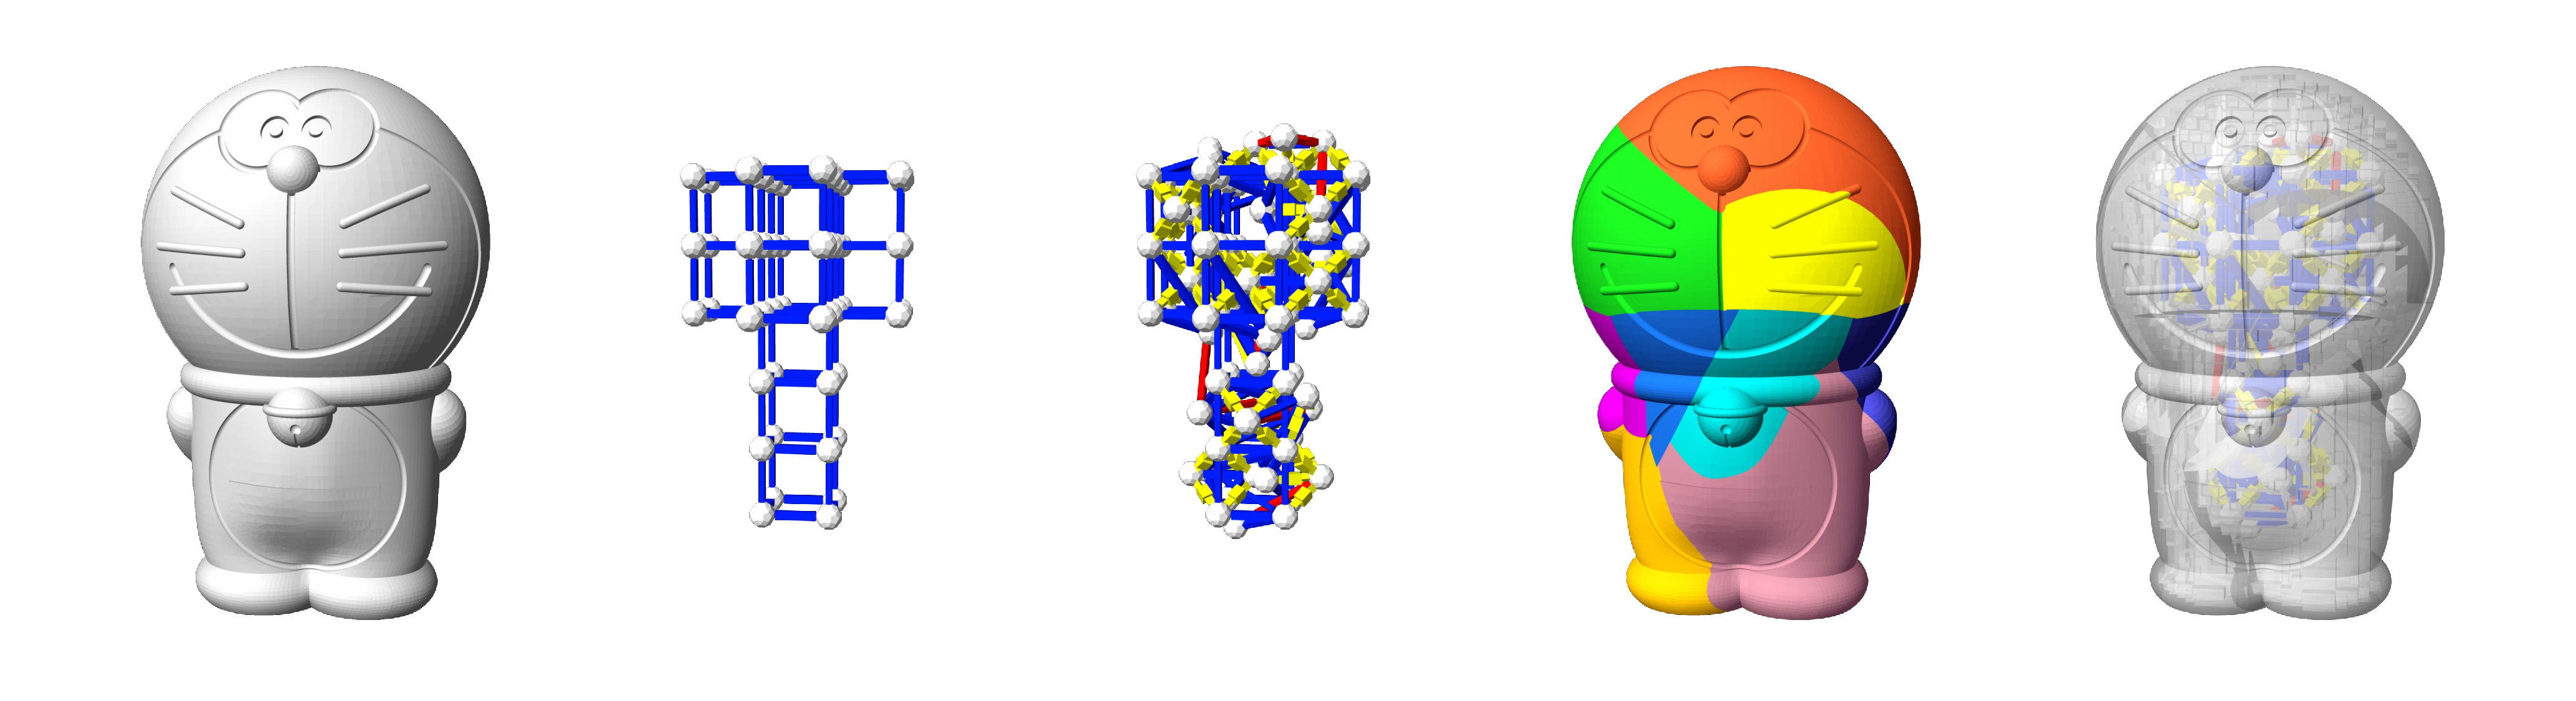
\includegraphics[width=1.0\linewidth]{figs/doraemon.pdf} 
%\caption{Result : Doraemon}
%\label{fig:result-assembly_doraemon}
%\end{figure*}

%\begin{figure*}[ht]
%\centering
%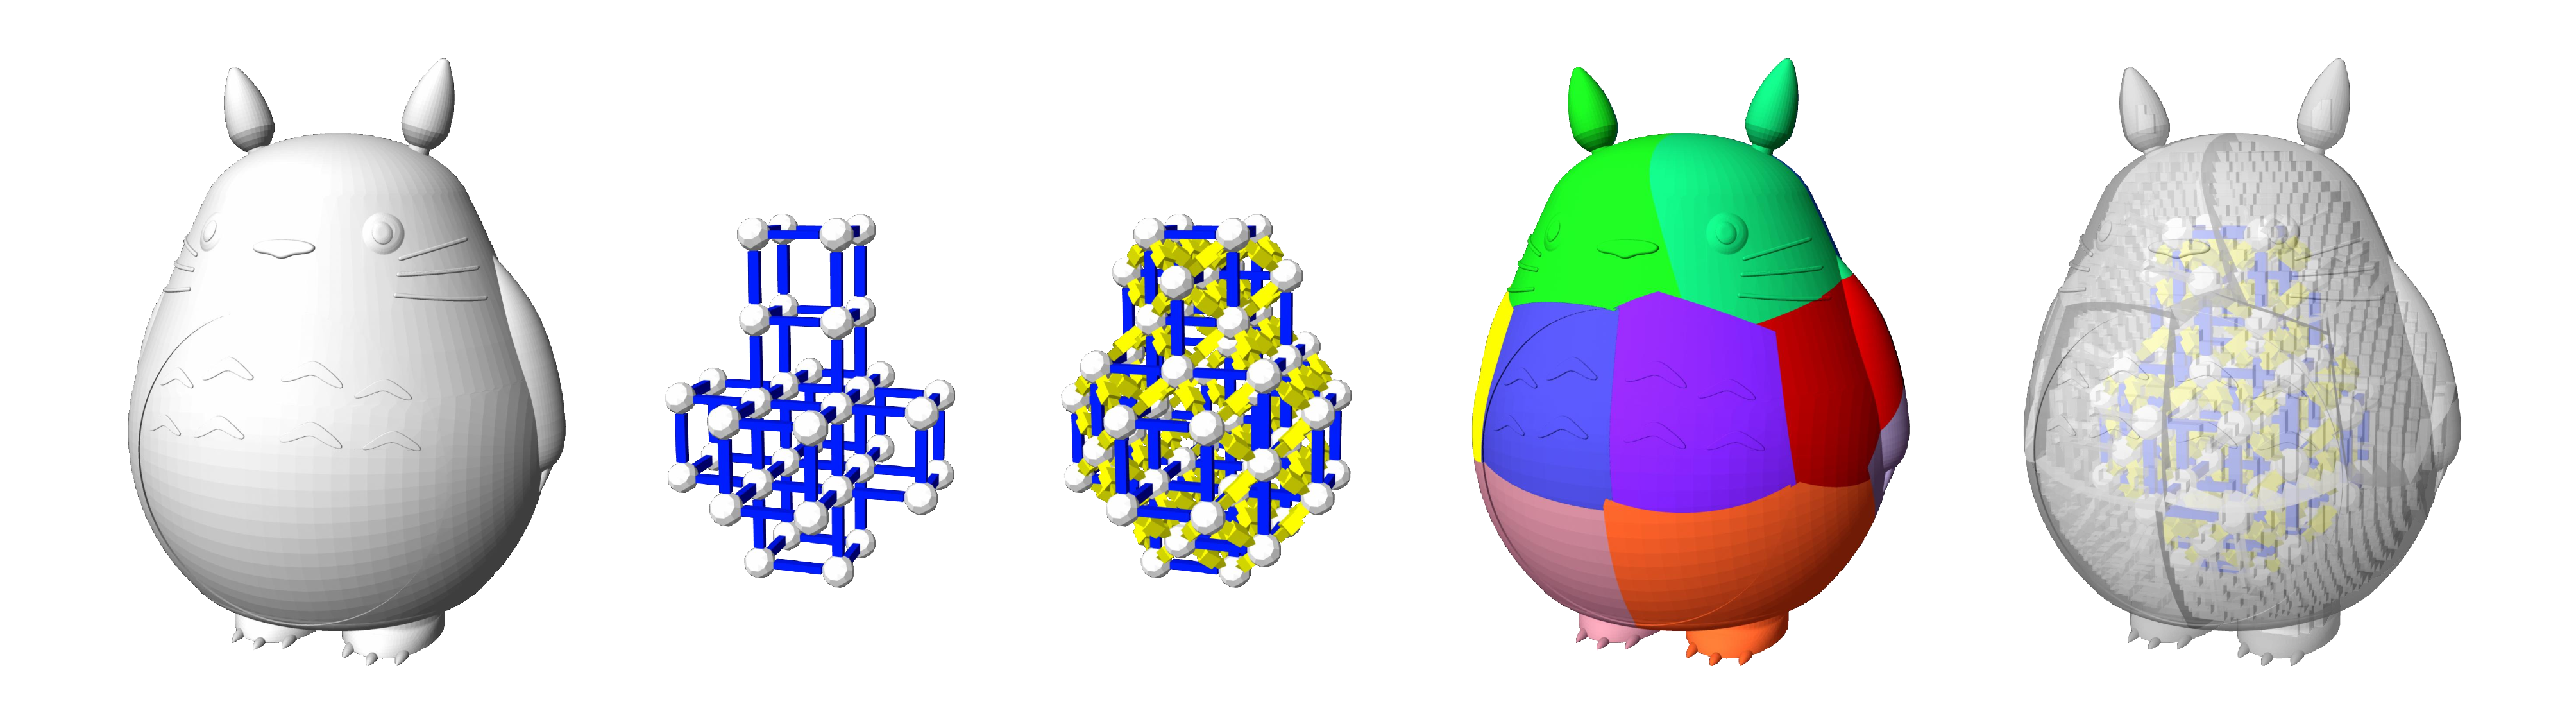
\includegraphics[width=1.0\linewidth]{figs/totoro.pdf} 
%\caption{Result : Totoro}
%\label{fig:result-assembly_totoro}
%\end{figure*}

%\begin{figure*}[ht]
%\centering
%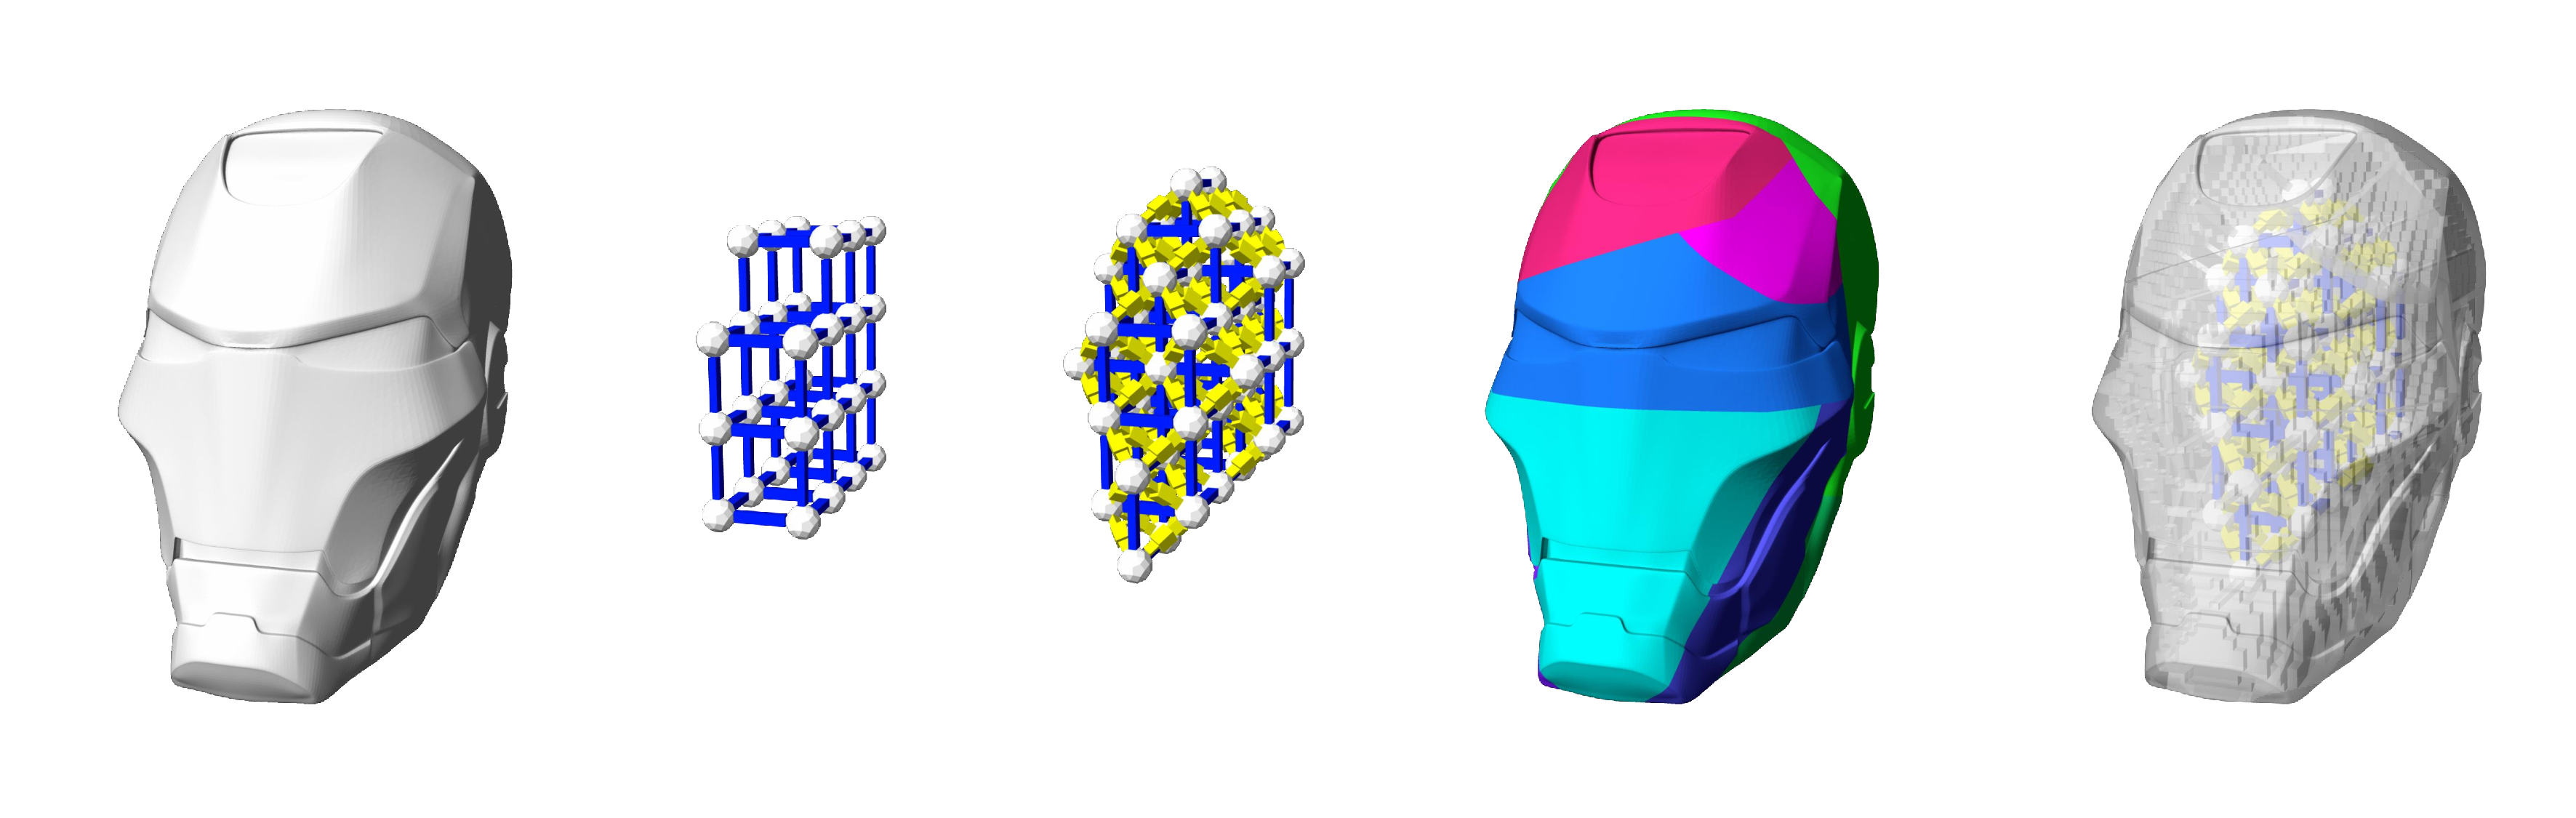
\includegraphics[width=1.0\linewidth]{figs/iron.pdf} 
%\caption{Result : Iron Man}
%\label{fig:result-assembly_iron}
%\end{figure*}

%\begin{figure*}[ht]
%\centering
%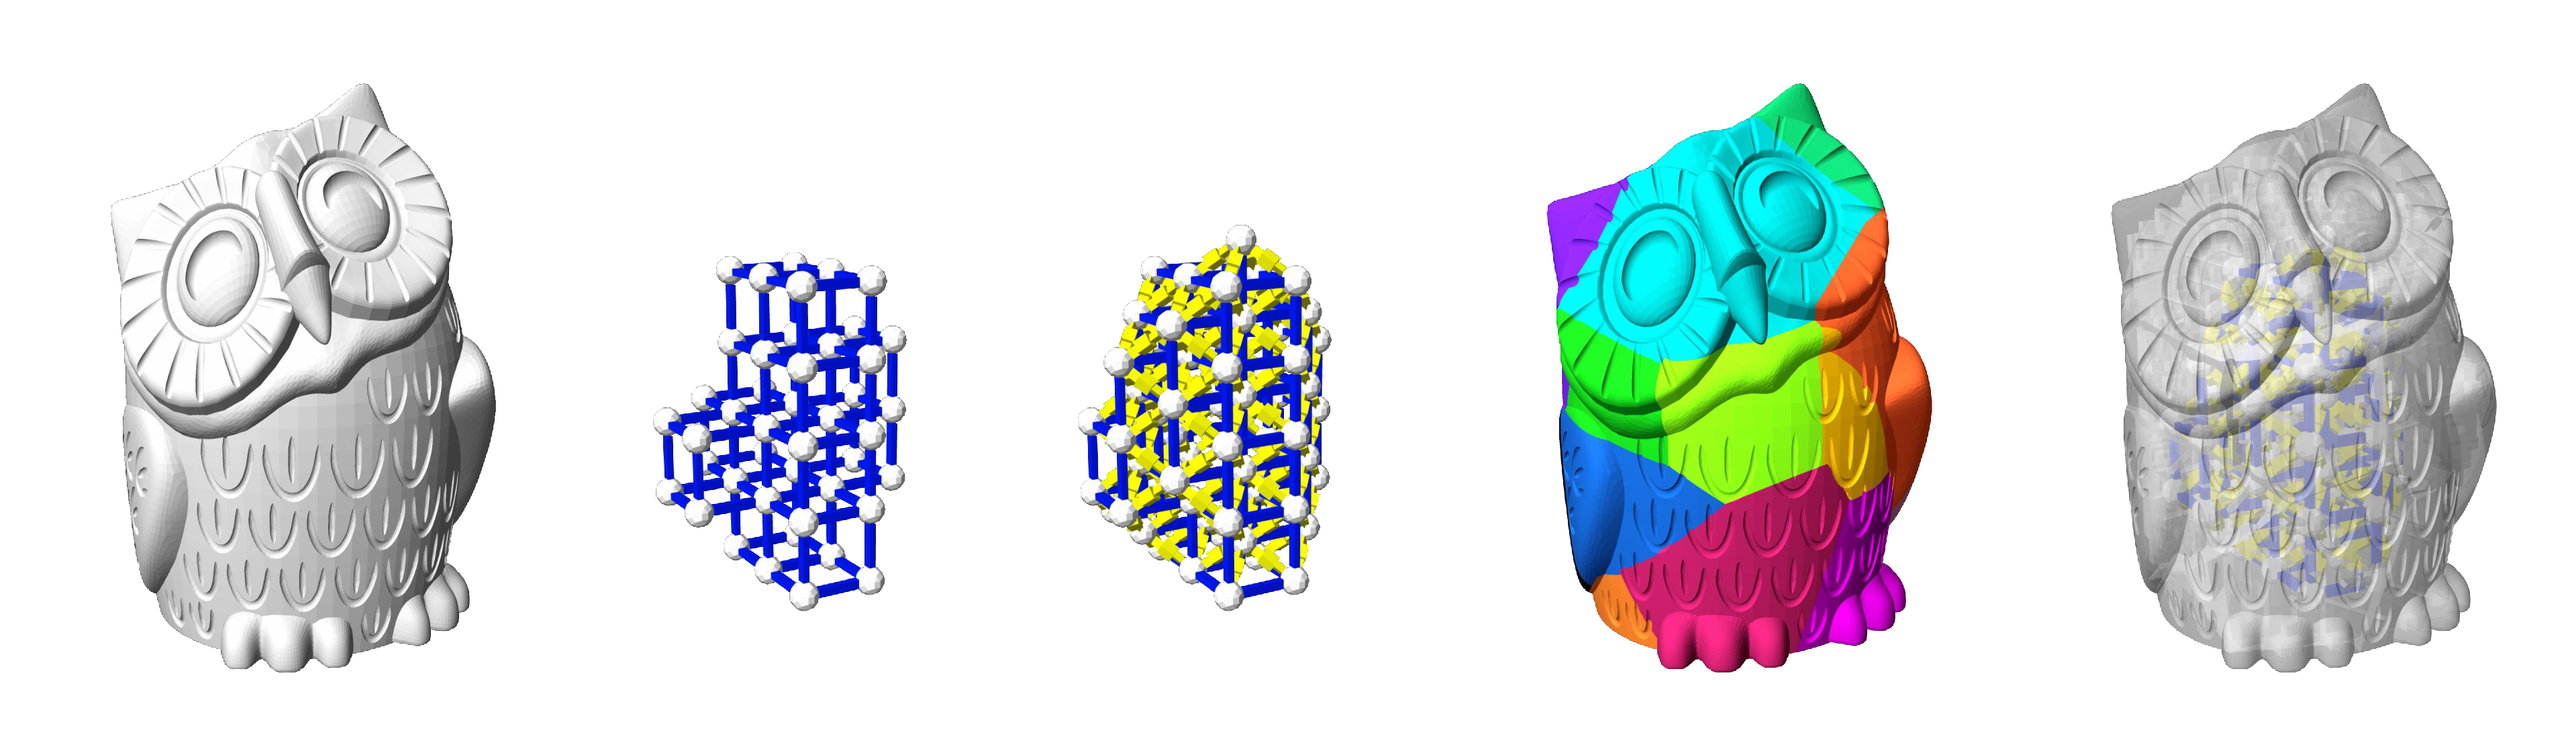
\includegraphics[width=1.0\linewidth]{figs/owl.pdf} 
%\caption{Result : Owl}
%\label{fig:result-assembly_owl}
%\end{figure*}

%\begin{figure*}[ht]
%\centering
%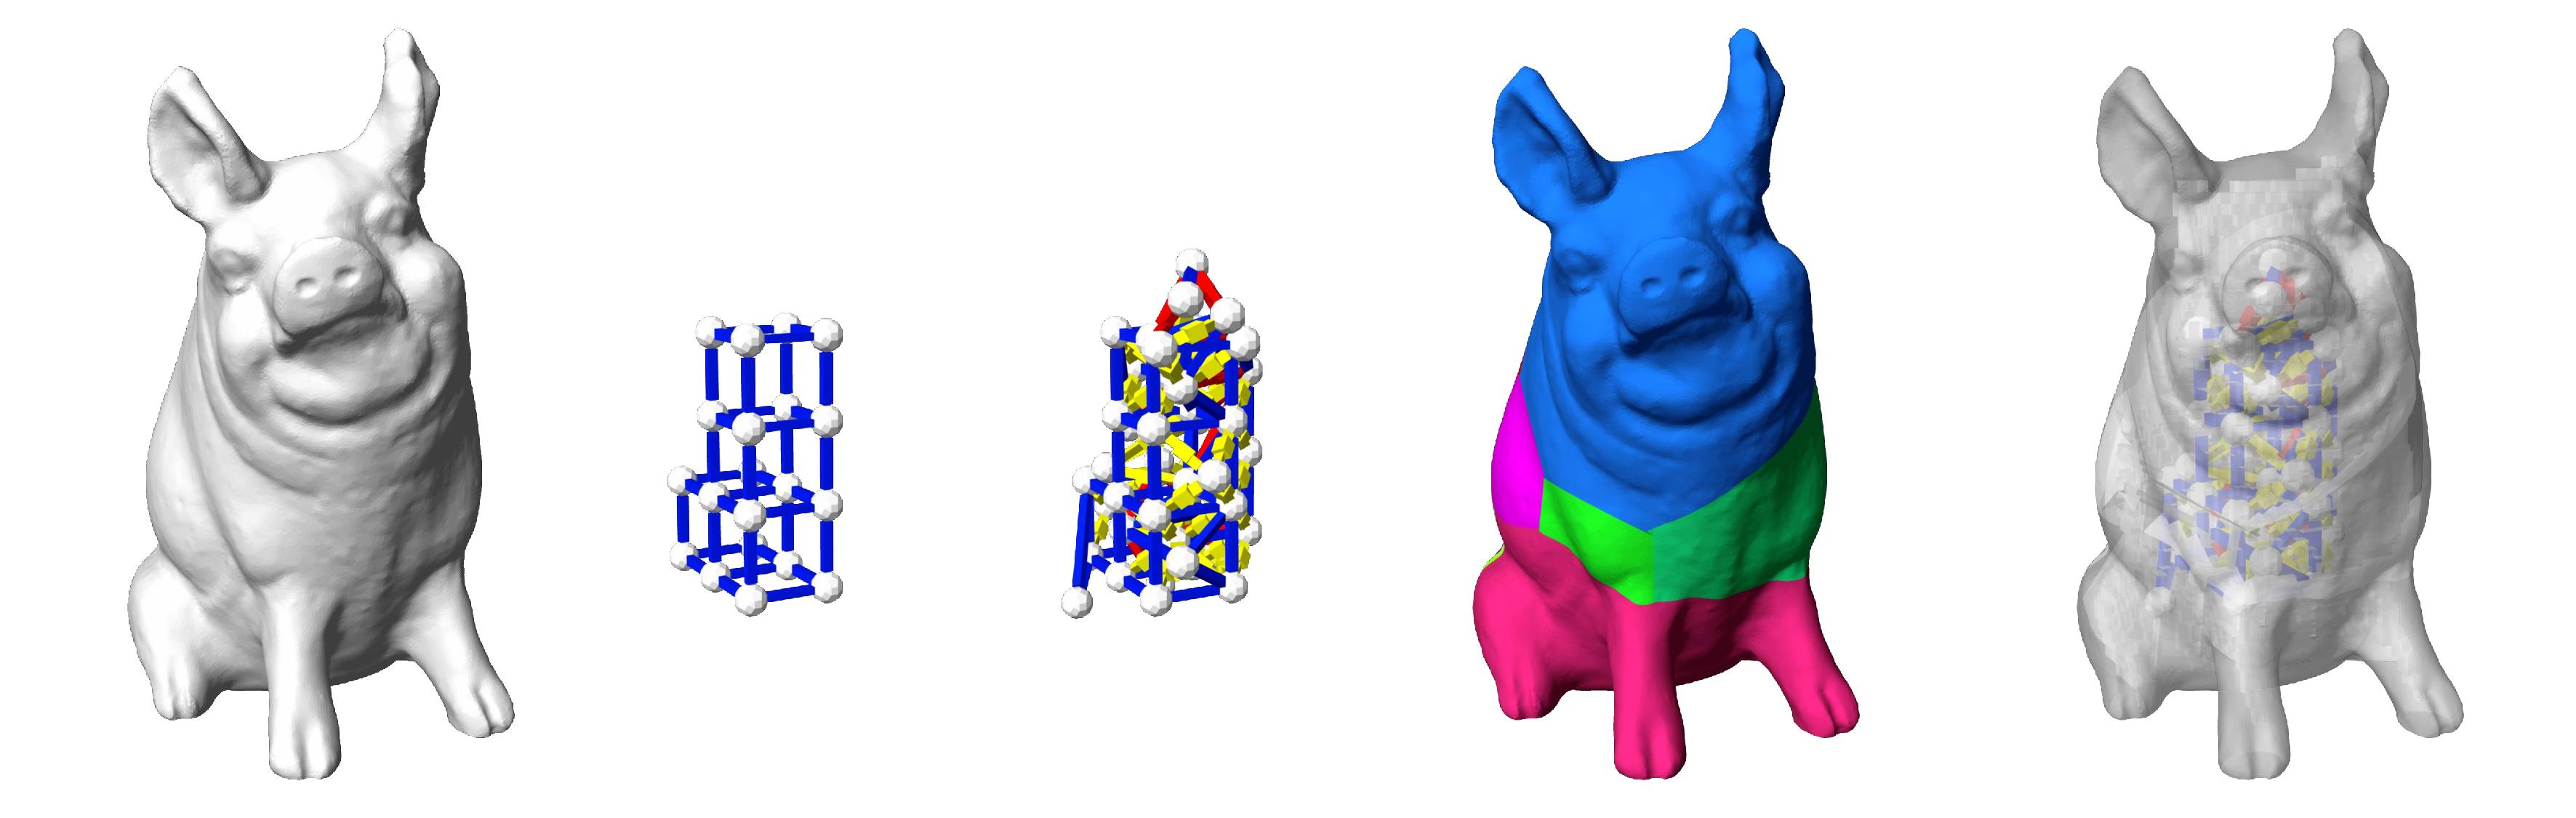
\includegraphics[width=1.0\linewidth]{figs/pig.pdf} 
%\caption{Result : Pig}
%\label{fig:result-assembly_pig}
%\end{figure*}

%\begin{figure*}[ht]
%\centering
%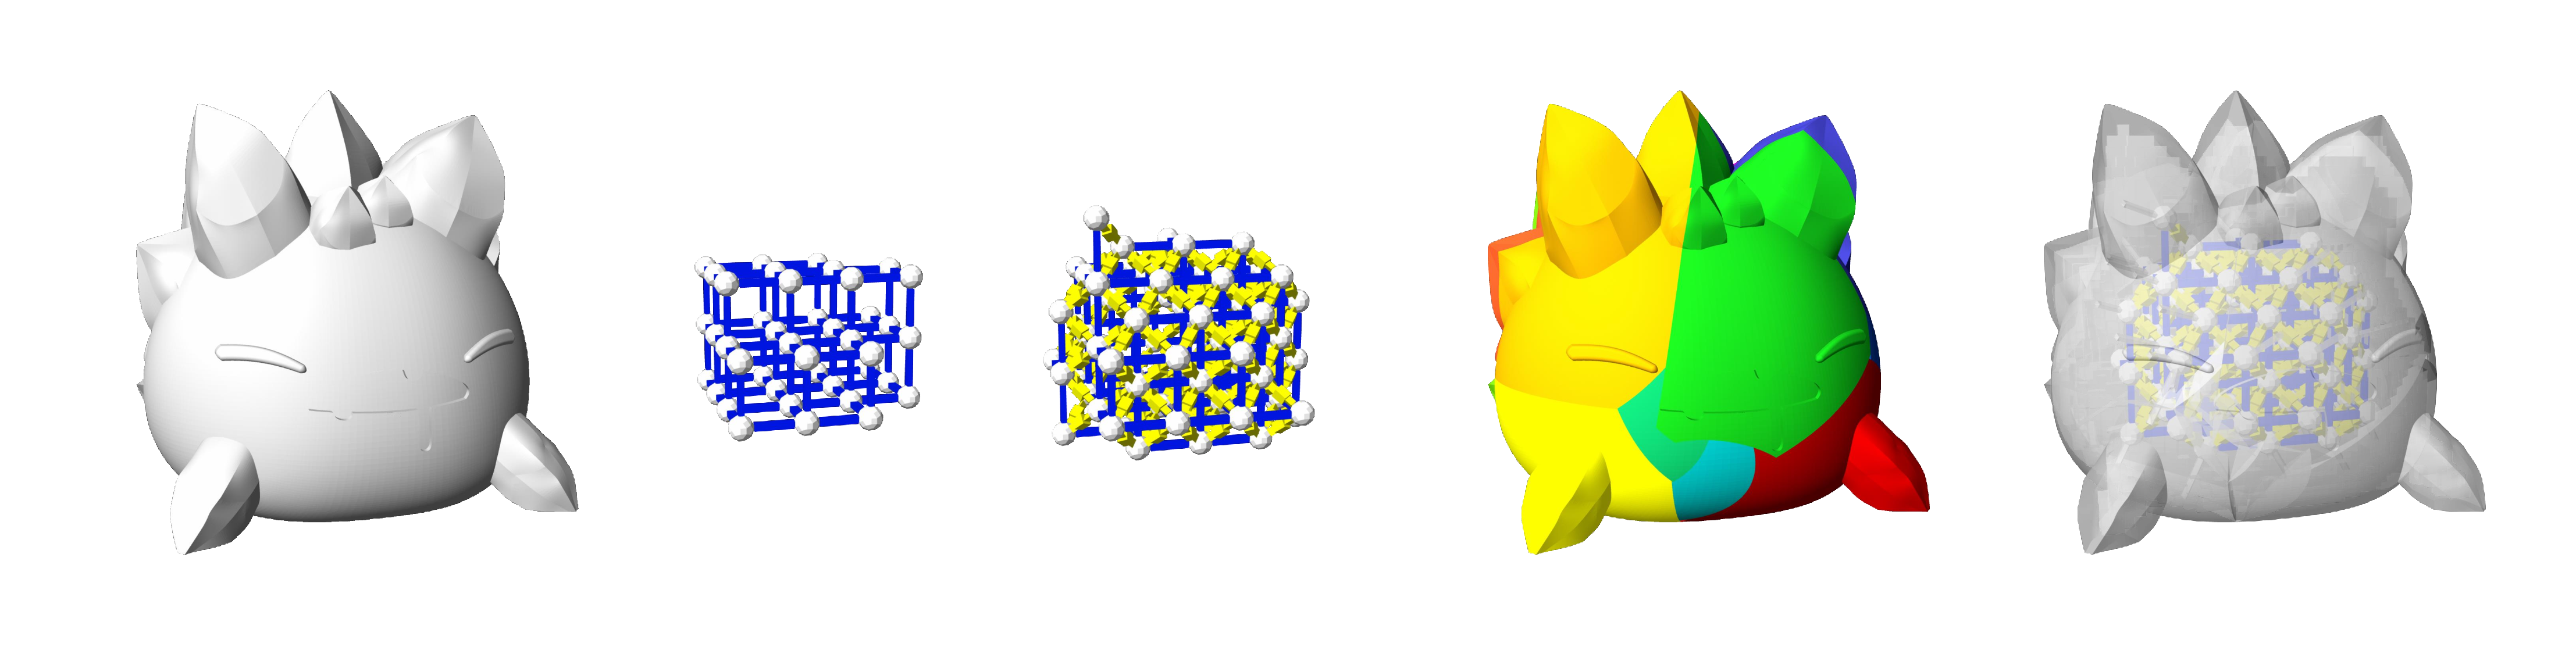
\includegraphics[width=1.0\linewidth]{figs/slime_high.pdf}
%\caption{Result : Slime}
%\label{fig:result-assembly_slime}
%\end{figure*}

%\begin{figure*}[ht]
%\centering
%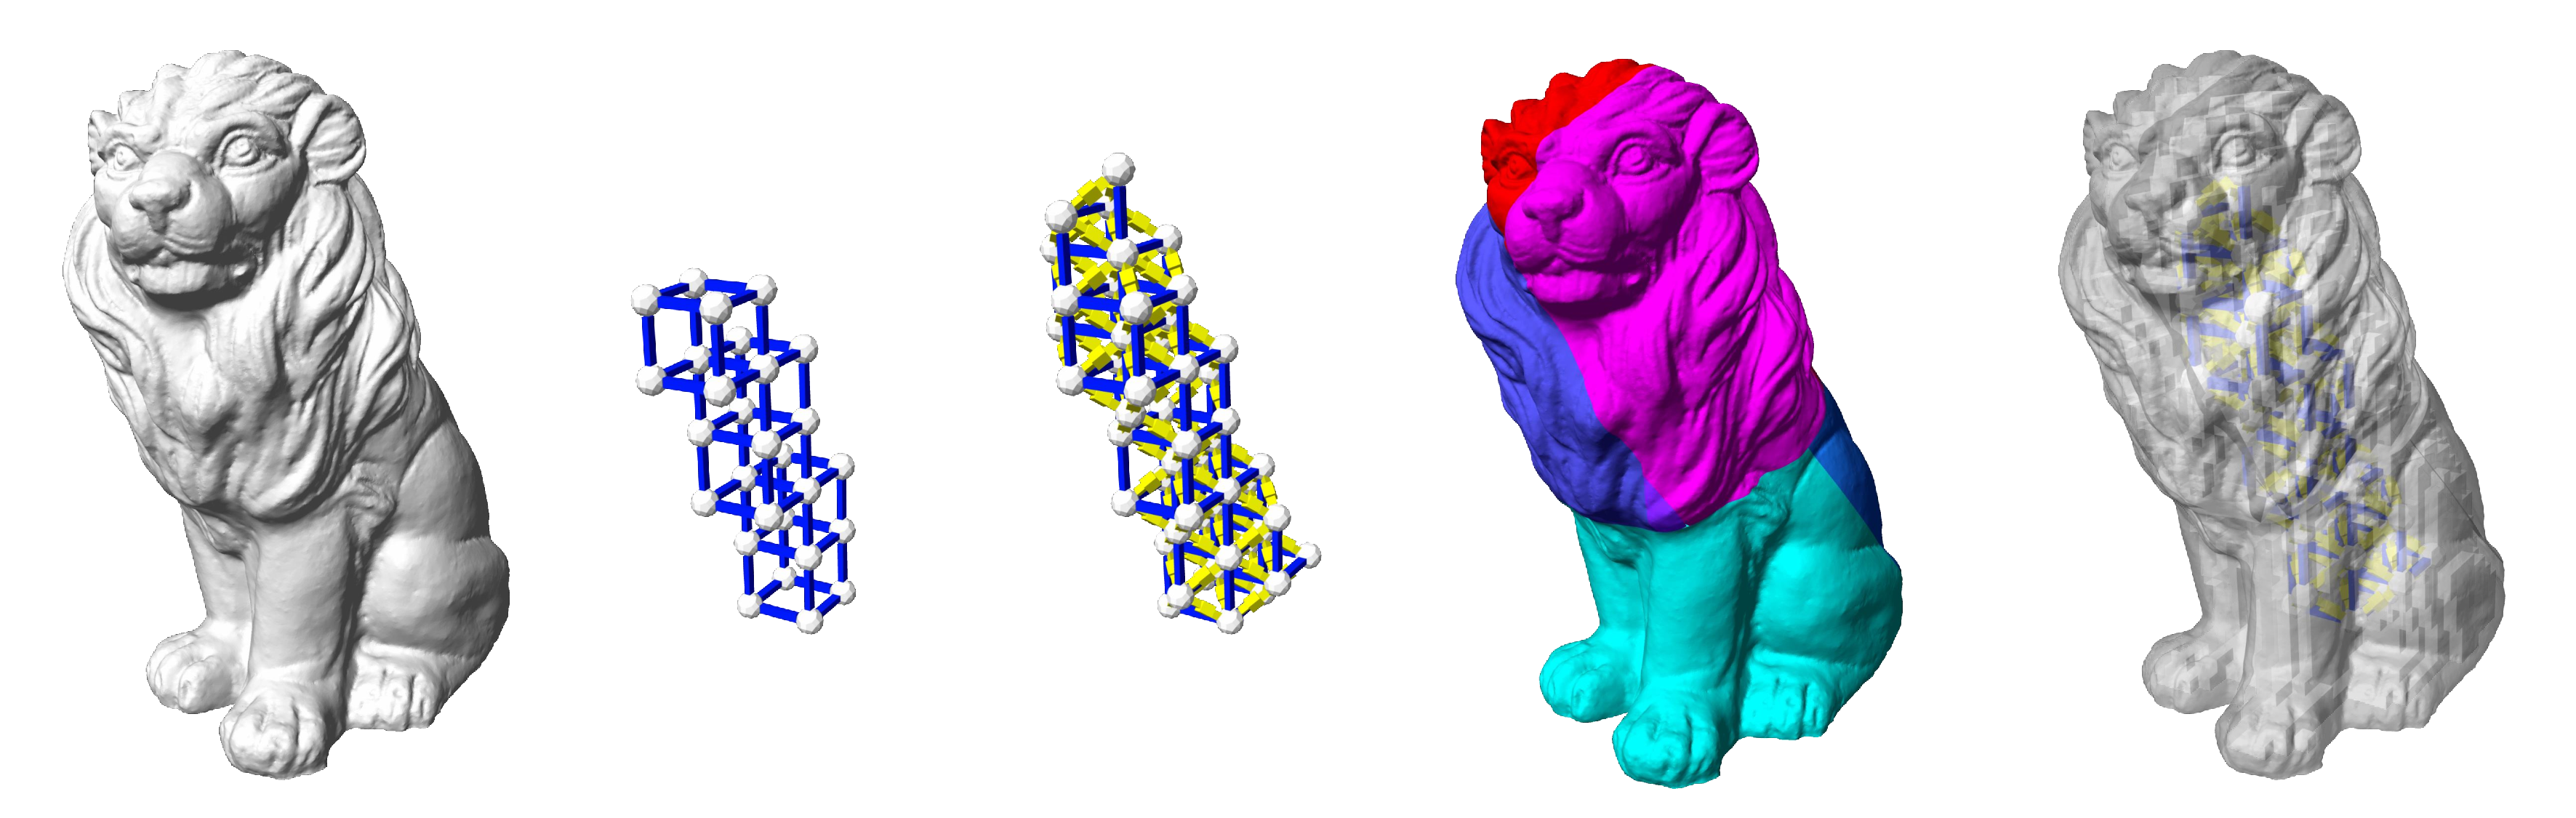
\includegraphics[width=1.0\linewidth]{figs/lion.pdf} 
%\caption{Result : Lion}
%\label{fig:result-assembly_lion}
%\end{figure*}

%\begin{figure*}[ht]
%\centering
%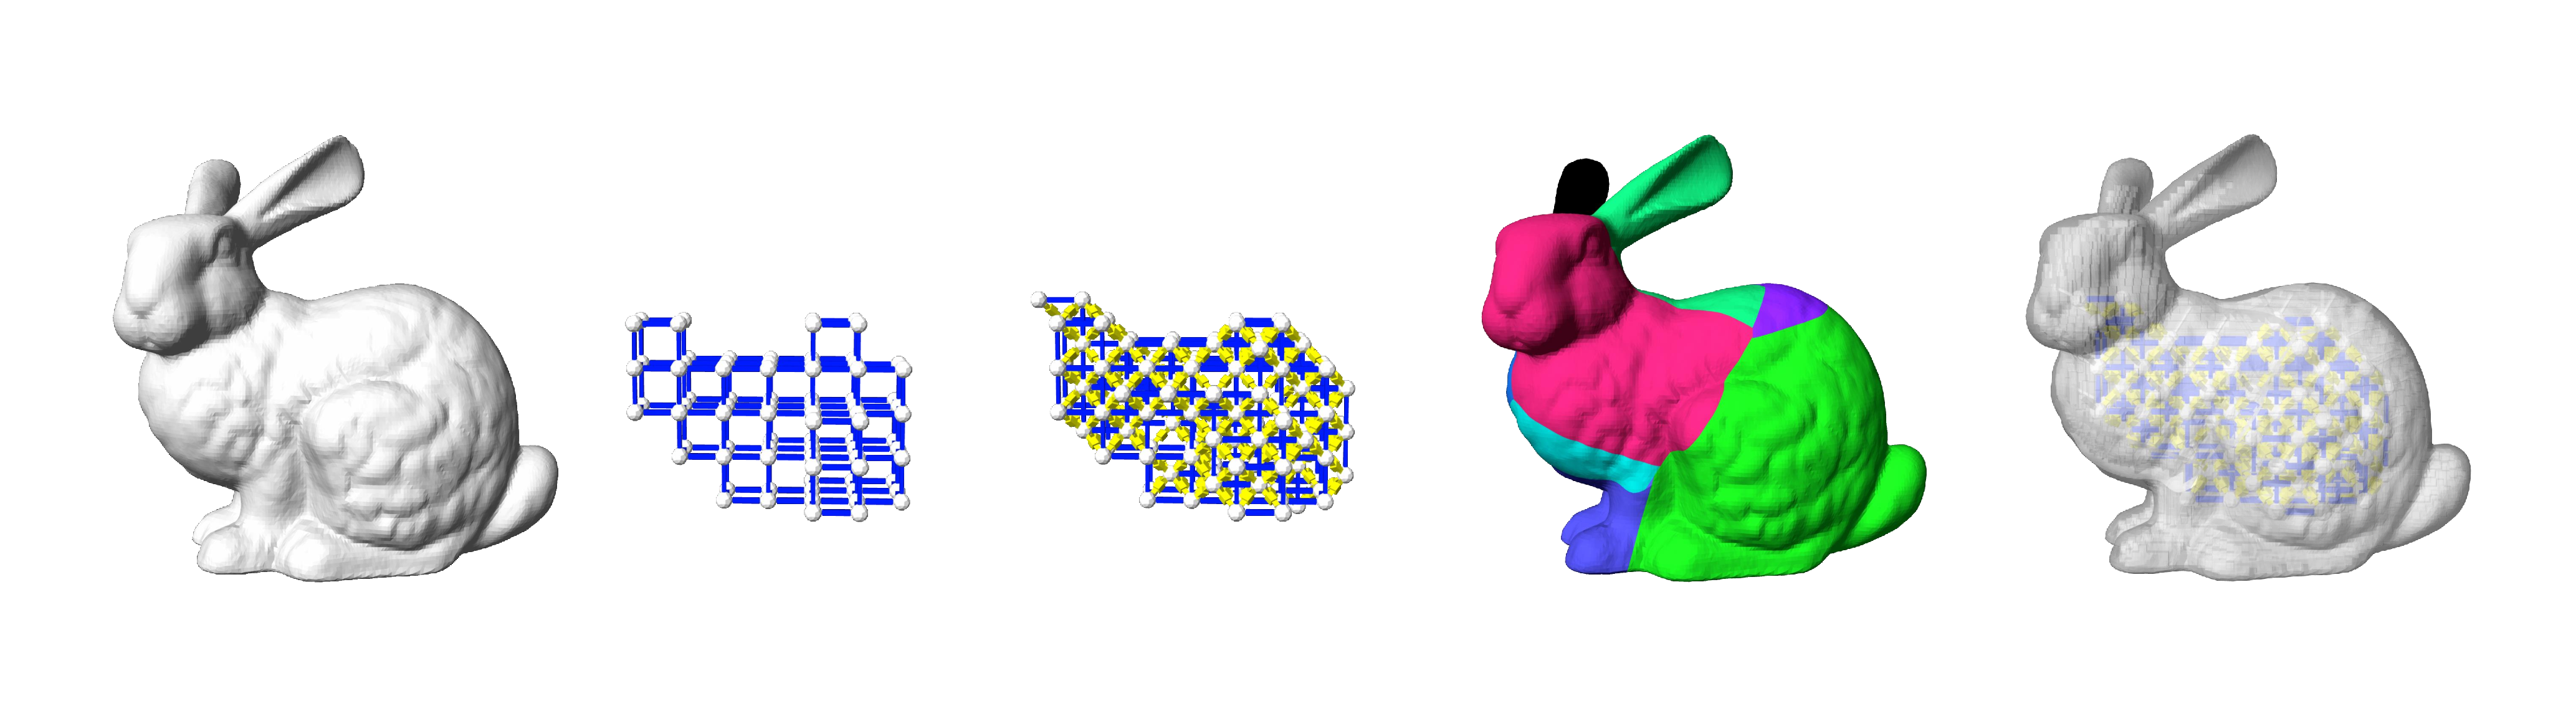
\includegraphics[width=1.0\linewidth]{figs/bunny_150.pdf} 
%\caption{Result : Bunny}
%\label{fig:result-assembly_Bunny}
%\end{figure*}

\section{Conclusion}
\label{sec:conclusion}

ZomeFab is method which combines Zometool and 3{D} printing to fabricate a large-scale 3{D} objects. In this approach, we aimed to represent an input 3D mesh by a inner structure and pieces of outer surfaces. Compare with print partitioned input mesh directly, the inner structure greatly saves the cost of 3D printing. The outer surfaces still remain the fine geometric characteristic of 3D printer. Thanks to the reusability of Zometool, the long-term cost of fabrication quite decreased. However, Zometool is a complex geometric system which can build thousands of structures. Our method generate a Zometool result which can simply build and also fit in well for outer surface. User can get the pretty well result by using Zomefab.

\subsection{Limitation}
%Zomefab relied on the input mesh which have the large inner volume and using Zometool as inner structure. The smallest Zometool cube (4.7cm x 4.7cm x 4.7cm) is limited. Therefore, in order to get the initial structure have to make sure input mesh's inner volume must larger than one unit cube. In the future, we can change the unit cube into different and smaller shape to get better structure fitting inside the mesh.

Though Zomefab can provide a method for user to design the large prototype with 3{D} printing and Zometool. But our method still has some limitations. As three conditions: 

\subsubsection{Big inner volume} 
Our initial structure, Zometool-cube, is a 4.7cm x 4.7cm x 4.7cm repeat structure. Therefore, in order to get the initial structure, we have to make sure that the input mesh's inner volume must larger than one unit cube. %(\figname~\ref{fig:limitation}(a))

\subsubsection{Multiple part of initial structure} 
Although Zometool have thousands of construct methods, it still has a mathematical model. It means that the construct method is finite. Multiple part of initial structure maybe can't find a Zometool connection path. It will make the balance of structure very dangerous. So we recommend user's input mesh just has single main structure. 
%(\figname~\ref{fig:limitation}(b))

\subsubsection{Thin part of input mesh} 
Our method doesn't have the analysis of balance. 
%Although the input mesh have a very large inner volume, if the mesh have to rely on the thin part lay on the surface, our system can't ensure the result whether can put on the surface perfectly. 
Even if the input mesh has a very large inner volume and have to rely on the thin parts which contact on the surface, our method don't have the balance analysis and can't ensure whether the result can put on the surface perfectly. 

%(\figname~\ref{fig:limitation}(a))
%\begin{figure*}[ht]
%\centering
%\includegraphics[width=1.0\linewidth]{figs/limitation.pdf} 
%\caption{Our method's limitations. (a) The mesh's inner volume is too small or the %mesh has the thin parts (b) Have multiple parts of initial structure}
%\label{fig:limitation}
%\end{figure*}

\subsection{Future work}
In order to handle our method's limitations, we have some following changes for our method:

\subsubsection{Change the smaller unit shape} 
Current repeated structure is a little bit bigger for common mesh. To let structure fit inside the mesh better, we have to think if there is another structure that is smaller and better than Zometool-cube.

\subsubsection{Handle multiple part of initial structure} 
Lots of mesh don't have a main big volume but have multiple parts which can put Zometool-cube in. One aspect is the balance problem, and the other is our growing tenon's method just can grow out one direction on one piece. We can modify the method to let the different parts of Zometool structures be connected by one printing piece. 

\subsubsection{Analyze the structure balance} 
Current method doesn't have balance analysis system. So our input mesh has to find some mesh that has large inner volume for our method. If we have balance analysis, we can analyze whether the structure is safe and modify the energy function of simulated annealing, then our result will be more robust.



% %% \section{Introduction} %for journal use above \firstsection{..} instead

\bibliographystyle{abbrv}
%%use following if all content of bibtex file should be shown
%\nocite{*}
\bibliography{zomeFab}
\end{document}
